\chapter{Measuring the Muon Neutrino Magnetic Moment}\label{sec:NeutrinoMagMoment}

\todo{Also check out NeutrinoMassesPheno2007.pdf, sec 6.4}

%%% ABSTRACT %%%
\todo{Write an introduction to the NuMM}
%"In the standard model, neutrinos have small charge radii induced by radiative corrections. The predicted values of the electron and muon neutrino charge radii are less than an order of magnitude smaller than the current experimental upper limits and can be tested in the next generation of accelerator and reactor experiments through the observation of neutrino-electron elastic scattering and CEvNS. Precision measurements of the neutrino charge radii would either be an important confirmation of the standard model, or would discover new physics. The same types of experimental measurements are also sensitive to more exotic neutrino electromagnetic properties: magnetic moments and millicharges, which would be certainly due to new BSM physics. The discovery of millicharges or anomalously large neutrino magnetic moments would have also important implications for astrophysics and cosmology."\cite{SnowmassNeutrinoFrontierReport.pdf}

%[SNOWMASSLOI_NuMMAtNuMuBeams.pdf] Extensions to the Standard Model predict neutrino magnetic moments[1-3], regardless of whether neutrinos are Dirac or Majorana particles. .. Such an unambiguous excess could be interpreted, for example, as evidence[3] for the Majorana nature of the neutrino.

\section{Theory of neutrino magnetic moment}
%Neutrino electromagnetic properties have been proposed since the very beginning by Pauli to solve the discrepancies in the electron beta emission spectra. This was solved by discovering the neutron. Then again, neutrino magnetic moment was proposed as one of the solution to the solar neutrino problem 

% Although in the standard model neutrinos are electrically neutral and do not possess electric or magnetic dipole moments, they have a charge radius which is generated by radiative corrections. [...] In many extensions of the standard model neutrinos also acquire electromagnetic properties through quantum loop effects which allow direct interactions of neutrinos with electromagnetic fields and electromagnetic interactions of neutrinos with charged particles. Hence, the theoretical and experimental study of neutrino electromagnetic interactions is a powerful tool in the search for the fundamental theory beyond the standard model. Moreover, the electromagnetic interactions of neutrinos can generate important effects, especially in astrophysical environments, where neutrinos propagate over long distances in magnetic fields in vacuum and in matter. [nuElmagInt2015.pdf]

% ...the existence of neutrino masses and mixing implies that neutrinos have magnetic moments. Since their values depend on the specific theory which extends the standard model in order to accommodate neutrino masses and mixing, experimentalists and theorists are eagerly looking for them. [nuElmagInt2015.pdf]

%Systematic theoretical studies of neutrino electromagnetic properties started after it was shown that in the extended standard model with right-handed neutrinos the magnetic moment of a massive neutrino is, in general, nonvanishing and that its value is determined by the neutrino mass (Lee and Shrock, 1977; Marciano and Sanda, 1977; Petcov, 1977; Fujikawa and Shrock, 1980; Pal and Wolfenstein, 1982; Shrock, 1982; Bilenky and Petcov, 1987). [nuElmagInt2015.pdf]

%Neutrino electromagnetic properties are important because they are directly connected to fundamentals of particle physics. For example, neutrino electromagnetic properties can be used to distinguish Dirac and Majorana neutrinos, because Dirac neutrinos can have both diagonal and off-diagonal magnetic and electric dipole moments, whereas only the off-diagonal ones are allowed for Majorana neutrinos (Schechter and Valle, 1981; Kayser, 1982, 1984; Nieves, 1982; Pal and Wolfenstein, 1982; Shrock, 1982). This is shown in detail in Secs. III.A and III.B. Another important case in which Dirac and Majorana neutrinos have quite different observable effects is the spin-flavor precession in an external magnetic field discussed in Sec. VI.B. Neutrino electromagnetic properties are also probes of new physics beyond the standard model, because in the standard model neutrinos can have only a charge radius (see Secs. III.C and VII.B). The discovery of other neutrino electromagnetic properties would be a signal of new physics beyond the standard model (Bell et al., 2005, 2006; Bell, 2007; Novales-Sanchez et al., 2008). [nuElmagInt2015.pdf]

As was describe in Sec.~\ref{sec:NeutrinoTheory}, neutrinos in the \gls{SM} are massless and electrically neutral particles. However, even \gls{SM} neutrinos can have electromagnetic interaction through loop diagrams involving charged leptons and the W boson. These interactions are described by the neutrino charge radius, described in section \ref{sec:otherNuElmagProperties} \todo{Re-write this since I'm not going to include the other elmag properties section} \cite{SnowmassNeutrinoFrontierReport.pdf}.

%But this is only the neutrino charge radius, not the neutrino electric or magnetic moment (maybe also the anapole moment) "Hence, in the standard model the form factor can be interpreted as a neutrino charge radius or as an anapole moment (or as a combination of both). The standard model theory of the neutrino charge radius has a long history, with some controversies which are shortly summarized in the following." [nuElmagInt2015.pdf - sec.VIIB]

%Various theories beyond the Standard Model
In general \gls{BSM} theories, considering interactions with a single photon as shown on Fig.~\ref{fig:FeynmanNuElmagDiagram}, neutrino electromagnetic interactions can be described by an \textit{effective} interaction Hamiltonian \cite{nuElmagInt2015.pdf}
\begin{equation}
\mathcal{H}^{\left(\nu\right)}_{em}\left(x\right)=\sum^N_{k,j=1}\overline{\nu}_k\left(x\right)\Lambda^{kj}_{\mu}\nu_j\left(x\right)A^{\mu}\left(x\right).
\end{equation}
Here $\nu_k\left(x\right), k = 1,...,N,$ are neutrino fields in the mass basis with $N$ neutrino mass states and $x$ denotes the position. $\Lambda^{kj}_{\mu}$ is a general vertex function and $A^{\mu}\left(x\right)$ is the electromagnetic field.

\begin{figure}[hbtp]
\centering
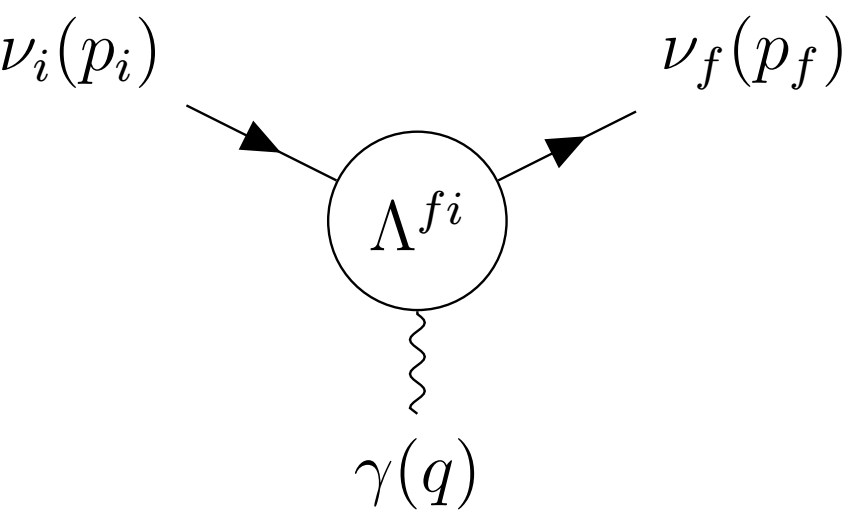
\includegraphics[width=0.4\linewidth]{Plots/NuMM/FeynmanDiagramNuElmagInt.png}
\caption{Effective coupling of neutrinos with one photon electromagnetic field.}
\label{fig:FeynmanNuElmagDiagram}
\end{figure}

\iffalse
The amplitude of neutrino-to-neutrino interaction for \textbf{Dirac} neutrinos is
\begin{equation}
\braket{\nu_f\left(p_f\right)|j^{\left(\nu\right)}_{\mu}\left(x\right)|\nu_i\left(p_i\right)}=
e^{i\left(p_f-p_i\right)x}\overline{u}_f\left(p_f\right)\Lambda^{fi}_{\mu}\left(p_f,p_i\right)u_i\left(p_i\right),
\end{equation}
where $p_f$ and $p_i$ are the final and initial four momentums respectively and $u/\overline{u}$ are the solutions to the Dirac equation for a free particle. We take into account possible transitions between different mass states $\nu_i$ and $\nu_f$ \cite{nuElmagInt2015.pdf}. \todo{also describe what is j}
\fi

The vertex function $\Lambda^{fi}_{\mu}\left(q\right)$ is generally a matrix and in the most general case consistent with the \gls{SM} gauge invariance \cite{MostGeneralNuElmagVectorFunctionExpressionKayser.pdf, MostGeneralNuElmagVectorFunctionExpressionNieves.pdf} can be written in terms of linearly independent products of Dirac matrices $\left(\gamma\right)$ and only depends on the four momentum of the photon $\left(q=p_f-p_i\right)$:
\begin{align}
\Lambda^{fi}_{\mu}\left(q\right)=&
\mathbb{F}^{fi}_1\left(q^2\right)q_{\mu}+
\mathbb{F}^{fi}_2\left(q^2\right)q_{\mu}\gamma_5+
\mathbb{F}^{fi}_3\left(q^2\right)\gamma_{\mu}+
\mathbb{F}^{fi}_4\left(q^2\right)\gamma_{\mu}\gamma_5+\notag\\ &
\mathbb{F}^{fi}_5\left(q^2\right)\sigma_{\mu\nu}q^{\nu}+
\mathbb{F}^{fi}_6\left(q^2\right)\epsilon_{\mu\nu\rho\gamma}q^{\nu}\sigma^{\rho\gamma},
\end{align}
where $\mathbb{F}^{fi}_i\left(q^2\right)$ are six Lorentz invariant form factors and $\delta$ and $\epsilon$ are the Dirac delta and the Levi-Civita symbols respectively.

Applying conditions of hermiticity $\left(\mathcal{H}^{\left(\nu\right)\dagger}_{em}=\mathcal{H}^{\left(\nu\right)}_{em}\right)$ and of the gauge invariance of the electromagnetic field, the vertex function can be rewritten as
\begin{equation}
\Lambda^{fi}_{\mu}\left(q\right)=
\left(\gamma_{\mu}-q_{\mu}\slashed{q}/q^2\right)\left[
\mathbb{F}^{fi}_{Q}\left(q^2\right)+\mathbb{F}^{fi}_{A}\left(q^2\right)q^2\gamma_5\right]-
i\sigma_{\mu\nu}q^{\nu}\left[\mathbb{F}^{fi}_{M}\left(q^2\right)+i\mathbb{F}^{fi}_{E}\left(q^2\right)\gamma_5\right],
\end{equation}
where $\mathbb{F}^{fi}_Q,\mathbb{F}^{fi}_M,\mathbb{F}^{fi}_E$ and $\mathbb{F}^{fi}_A$ are hermitian matrices representing the charge, dipole magnetic, dipole electric and anapole neutrino form factors respectively. It is clear that the vertex function only depends on the square of the four momentum of the photon $q^2$. In coupling with a real photon $\left(q^2=0\right)$ these form factors become the neutrino charge and magnetic, electric and anapole moments. The neutrino charge radius corresponds to the second term in the expansion of the charge form factor \cite{nuElmagInt2015.pdf}.

The above expression can be simplified as \cite{NeutrinoPropertiesSnowmass2022.pdf}
\begin{equation}
\Lambda^{fi}_{\mu}\left(q\right)=\gamma_{\mu}\left(Q_{\nu_{fi}}+\frac{q^2}{6}\langle r^2\rangle_{\nu_{fi}}\right)-i\sigma_{\mu\nu}q^{\nu}\mu_{\nu_{fi}},
\end{equation}
where $Q_{\nu_{fi}}$, $\langle r^2\rangle_{\nu_{fi}}$, and $\mu_{\nu_{fi}}$ are the neutrino charge, effective charge radius (also containing anapole moment), and an effective magnetic moment (also containing electric moment) respectively. This is possible thanks to the similar effect of the neutrino charge radius and the anapole moment, or of the neutrino magnetic and electric moment respectively \cite{nuElmagInt2015.pdf}. These are the three neutrino electromagnetic properties (charge, charge radius and magnetic moment) measured in the experiments.

\todo{Add a note briefly describing the other elmag properties and mentioning that they could be measured as well, but not describe here. Maybe refer reader to the theoretical overview paper}

\iffalse
For antineutrinos the form factors are transformed as:
\begin{equation}\label{eqAnu1}
\overline{\mathbb{F}}^{fi}_{\Omega}=-\mathbb{F}^{if}_{\Omega}=-\left(\mathbb{F}^{fi}_{\Omega}\right)^{\star} \ \ \ \Omega=Q,M,E,
\end{equation}
\begin{equation}\label{eqAnu2}
\overline{\mathbb{F}}^{fi}_{A}=\mathbb{F}^{if}_{A}=\left(\mathbb{F}^{fi}_{A}\right)^{\star}.
\end{equation}
\todo{maybe describe what does this mean?}

In case of \textbf{Majorana neutrinos}, the general expression for the vertex function in terms of charge, magnetic, electric and anapole form factors looks the same as for Dirac neutrinos.
\todo{so does that mean that the interaction amplitude can be written in the same way for both Dirac and Majorana neutrinos?} However, since Majorana antineutrinos are the same particle as Majorana neutrinos, from eq.\ref{eqAnu1},\ref{eqAnu2} we can see that:
\begin{equation}\label{eqAntisymmetryCondition}
\mathbb{F}^M_{\Omega}=-\left(\mathbb{F}^M_{\Omega}\right)^T \ \ \ \Omega=Q,M,E,
\end{equation}
\begin{equation}
\mathbb{F}^M_{A}=\left(\mathbb{F}^M_A\right)^T.
\end{equation}
Therefore the Majorana charge, magnetic and electric form factor matrices are antisymmetric and the anapole form factor matrix is symmetric. This means that Majorana neutrino doesn't have any diagonal charge and dipole magnetic and electric moments, but it can have transition  charge and magnetic and electric moment \cite{nuElmagInt2015.pdf}.
\todo{Explain why is this worth mentioning or remove it if it's not}
\fi

%%%%%%%%%%%%%%%%%%%%%%%%%%%%%%%%%%%%%%%%
\subsection{Neutrino electric and magnetic dipole moments}
The size and effect of neutrino electromagnetic properties depend on the specific \gls{BSM} theory. Evaluating the one loop diagrams in the minimally extended \gls{SM} with three right-handed Dirac neutrinos as described in Sec.~\ref{sec:NuMass} gives the first approximation of the electric and magnetic moments:
\begin{equation}\label{eq:DiracMagMomExpression}
\begin{rcases}
\mu^D_{kj}\\
i\epsilon^D_{kj}
\end{rcases}
\simeq\frac{3eG_F}{16\sqrt{2}\pi^2}\left(m_k\pm m_j\right)\left(\delta_{kj}-\frac{1}{2}\sum_{l=e,\mu ,\tau}U^{\star}_{lk}U_{lj}\frac{m_l^2}{m_W^2}\right),
\end{equation}
where $m_k,m_j$ are the neutrino masses and $m_l$ are the masses of charged leptons which appear in the loop diagrams \cite{nuElmagInt2015.pdf}. Also, $D$ superscript denotes Dirac neutrinos, $e$ is the electron charge, $G_F$ is the Fermi coupling constant, and $U$ is the \gls{PMNS} neutrino oscillation matrix. Higher order electromagnetic corrections were neglected, but can also have a significant contribution, depending on the theory.

It can be seen that Dirac neutrinos have no diagonal electric moments $\left(\epsilon_{kk}^D=0\right)$ and their diagonal magnetic moments are approximately
\begin{equation}\label{eq:DiagMagMomVal}
\mu_{kk}^D\simeq\frac{3eG_Fm_k}{8\sqrt{2}\pi^2}\simeq 3.2\times 10^{-19}\left(\frac{m_k}{\textsf{eV}}\right)\mu_B,
\end{equation}
where $\mu_B$ is the Bohr magneton which represents the value of the electron magnetic moment \cite{nuElmagInt2015.pdf}. Neutrino magnetic moments are therefore strongly suppressed by the smallness of neutrino masses, with theoretical predictions in Eq.~\ref{eq:DiagMagMomVal} several orders of magnitude below the reach of current experiments \cite{NeutrinoPropertiesSnowmass2022.pdf}.

The transition magnetic moments from Eq.~\ref{eq:DiracMagMomExpression} are suppressed with respect to the largest of the diagonal magnetic moments by at least a factor of $10^{-4}$ due to the $m_W^2$ in the denominator. The transition electric moments are even smaller due to the mass difference in Eq.~\ref{eq:DiracMagMomExpression}. Therefore an experimental observation of a magnetic moment larger than in Eq.~\ref{eq:DiagMagMomVal} would indicate physics beyond the minimally extended \gls{SM} \cite{nuElmagInt2015.pdf,nuMMMajoranaBounds2006.pdf}.

\todo{Actually write why these values are different for Majorana neutrinos than for Dirac neutrinos}
Majorana neutrinos in a minimal extension can be obtained by either adding a $\textsf{SU}\left(2\right)_L$ Higgs triplet, or right handed neutrinos together with a $\textsf{SU}\left(2\right)_L$ Higgs singlet \cite{nuElmagInt2015.pdf}. If we neglect the Feynman diagrams which depend on the model of the scalar sector, the magnetic and electric dipole moments are
\begin{equation}
\mu_{kj}^M\simeq -\frac{3ieG_F}{16\sqrt{2}\pi^2}\left(m_k+m_j\right)\sum_{l=e,\mu ,\tau}\operatorname{Im}\left[U^{\star}_{lk}U_{lj}\right]\frac{m_l^2}{m_W^2},
\end{equation}
\begin{equation}
\epsilon_{kj}^M\simeq \frac{3ieG_F}{16\sqrt{2}\pi^2}\left(m_k-m_j\right)\sum_{l=e,\mu ,\tau}\operatorname{Re}\left[U^{\star}_{lk}U_{lj}\right]\frac{m_l^2}{m_W^2}.
\end{equation}
These are difficult to compare to the Dirac case, due to possible presence of Majorana phases in the \gls{PMNS} matrices, but it is clear that they have the same order of magnitude as Dirac transition dipole moments. However, the neglected model dependent contributions can enhance the transition dipole moments \cite{nuElmagInt2015.pdf}.

\todo{Re-read the natural upper bounds paper}
It is possible \cite{nuMMMajoranaBounds2006.pdf} to obtain a `natural' upper limits on the size of the neutrino magnetic moment by calculating its contribution to the neutrino mass by standard model radiative corrections. \todo{I don't think this is clear enough, how is this done} For Dirac neutrinos, the radiative correction induced by neutrino magnetic moment, generated at an energy scale $\Lambda_{NP}$, to the neutrino mass is generically
\begin{equation}
m_{\nu}^D\sim\frac{\mu_{\nu}^D}{3\times 10^{-15}\mu_B}\left[\Lambda\left(\textsf{TeV}\right)\right]^2\textsf{eV}.
\end{equation}
So for $\Lambda_{NP}\simeq 1\textsf{TeV}$ and $m_{\nu}\lesssim 0.3\textsf{eV}$ the limit becomes $\mu_{\nu}^D\lesssim 10^{-15}\mu_B$. This applies only if \gls{NP} is well above the electroweak scale ($\Lambda_{EW} \sim 100\textsf{GeV}$) \todo{Finish this sentence}. However, there are theories that contain a Dirac neutrino magnetic moment higher than this limit, for example in frameworks of minimal super-symmetric standard model, by adding more Higgs doublets, or by considering large extra dimensions \todo{Add references to the specific theories?} \cite{nuElmagInt2015.pdf}.

Similar limit for Majorana neutrino magnetic moment would be less stringent than for Dirac neutrinos due to the antisymmetry of the Majorana neutrino magnetic moment form factors \todo{Probably explain here a bit more what does this mean}. Considering $m_{\nu}\lesssim 0.3\textsf{eV}$, the limit can be expressed as 
\begin{align}
\mu_{\tau\mu},\mu_{\tau e} &\lesssim 10^{-9}\left[\Lambda\left(\textsf{TeV}\right)\right]^{-2}\\
\mu_{\mu e} &\lesssim 3\times 10^{-7}\left[\Lambda\left(\textsf{TeV}\right)\right]^{-2}
\end{align}
which is shown in the flavour basis \todo{Explain here what is the flavour basis}, which relates to the framework used previously via the \gls{PMNS} matrix as
\begin{equation}
\mu_{ij}=\sum_{\alpha\beta}\mu_{\alpha\beta}U^{\star}_{\alpha i}U_{\beta j},\ \ \ \alpha,\beta\in\left\lbrace e,\mu,\tau\right\rbrace.
\end{equation}

\todo{Add a discussion about the triangular inequalities}

These considerations imply, that if a magnetic moment $\mu\gtrsim 10^{-15}\mu_B$ would be measured, it is more plausible that neutrinos are Majorana fermions and that the scale of lepton violation would be well below the conventional see-saw scale \cite{nuMMMajoranaBounds2006.pdf} \todo{double check this claim, also reword this sentence}.

\subsubsection{Effective neutrino magnetic moment}
Since experiments detect neutrino flavour states, not the mass states, what we measure is an effective `flavour' magnetic moment $\mu_{eff}$. $\mu_{eff}$ is influenced by mixing of the neutrino magnetic moments (and electric moments) expressed in the mass basis (as described above) and neutrino oscillations \todo{This basis relation was already partly described above, mention that and combine the descriptions}. In the ultra-relativistic limit, the neutrino effective magnetic moment is
\begin{equation}
\mu_{\nu_l}^2\left(L,E_{\nu}\right)=\sum_j\left|\sum_k U^{\star}_{lk}e^{\mp i\Delta m^2_{kj}L/2E_{\nu}}\left(\mu_{jk}-i\epsilon_{jk}\right)\right|^2,
\end{equation}
where the minus sign in the exponent is for neutrinos and the plus sign for antineutrinos \cite{nuElmagInt2015.pdf}. Therefore the only difference between the effective neutrino and antineutrinos magnetic moment is in the phase induced by neutrino oscillations.

For experiments with baselines short enough that neutrino oscillations would not have time to develop $\left(\Delta m^2L/2E_{\nu}\ll\sim1\right)$, such as the \gls{NOvA} \gls{ND}, the effective magnetic moment can be expressed as
\begin{equation}
\mu_{\nu_l}^2=\mu_{\overline{\nu}_l}^2\simeq\sum_j\left|\sum_k U_{lk}^{\star}\left(\mu_{jk}-i\epsilon_{jk}\right)\right|^2=\left[U\left(\mu^2+\epsilon^2\right)U^{\dagger}+2\operatorname{Im}\left(U\mu\epsilon U^{\dagger}\right)\right]_{ll^{\prime}},
\end{equation}
which is independent of the neutrino energy \todo{Figure out how does this relate to the mag moment cross section which does depend on the neutrino energy!}.

\todo{Consider if this paragraph is actually important}
Since the effective magnetic moment depends on the flavour of the studied neutrino, it is different (but related) for neutrino experiments studying neutrinos from different sources. Additionally some experiments, namely solar neutrino experiments, need to include matter effects on the neutrino oscillations. Therefore the reports on the value (or upper limit) of the effective neutrino magnetic moment are not directly comparable between different types of neutrino experiments. Theorists publish papers trying to extrapolate the measured effective magnetic moments to each neutrino flavour, but necessarily apply assumptions that might not hold in all \gls{BSM} theories.

\subsection{Other neutrino electromagnetic properties}\label{sec:otherNuElmagProperties}
\note{I am not going to report results on these, so should I even mention them here? Maybe it's enough to just mention that they exist in the intro section...}
\todo{This section is not finished, most of this text is just copied from some theory papers for now}

\todo{See also StatusAndPerspectiveOfNuMM2016.pdf}

Neutrino electric charge is heavily constraint by the measurements on the neutrality of matter (since generally neutrinos having an electric charge would also mean that neutrons have charge which would affect all heavier nuclei). It is also constrained by the SN1987A, since neutrino having an effective charge would lengthen its path through the extragalactic magnetic fields and would arrive on earth later. It can also be obtained from nu-on-e scatter from the relationship between neutrino millicharge and magnetic moment. [nuElmagInt2015.pdf - sec. VIIA] \todo{Make this description shorter, just a single sentence and combine with the charge radius}

The neutrino charge radius is determined by the second term in the expansion of the neutrino charge form factor and can be interpreted using the Fourier transform of a spherically symmetric charge distribution. It can also be negative since the charge density is not a positively defined quantity. In the SM the charge radius has the form of (possible other definitions exist)
\begin{equation}
\langle r_{\nu_l}^2\rangle_{\textsf{SM}}=\frac{G_{\textsf{F}}}{4\sqrt{2}\pi^2}\left[3-2\log\left(\frac{m_l^2}{m_W^2}\right)\right].
\end{equation}
This corresponds to $\langle r_{\nu_{\mu}}^2\rangle_{\textsf{SM}}=2.4\times 10^{-33}\ \unit{cm^2}$ and similar scale for other neutrino flavours. [nuElmagInt2015.pdf - sec. VIIB]

[nuElmagInt2015.pdf - sec. VIIB]
The effect of the neutrino charge radius on the neutrino-on-electron scattering cross section is through the following shift of the vector coupling constant (Grau and Grifols, 1986; Degrassi, Sirlin, and VMarciano, 1989; Vogel and Engel, 1989; Hagiwara et al., 1994):
\begin{equation}
g_V^{\nu_l}\rightarrow g_V^{\nu_l}+\frac{2}{3}m_W^2\langle r_{\nu_l}^2\rangle\sin^2\theta_W
\end{equation}

[nuElmagInt2015.pdf - sec. VIIB]
The current experimental limits for muon neutrinos are from \todo{check the current exp. limits}  Hirsch, Nardi, and Restrepo (2003) who obtained the
following 90\% C.L. bounds on $\langle r_{\nu_\mu}^2\rangle$ from a reanalysis of
CHARM-II (Vilain et al., 1995) and CCFR (McFarland et al.,1998) data:
\begin{equation}
-0.52\times 10^{-32}<\langle r_{\nu_\mu}^2\rangle<0.68\times 10^{-32}\ \unit{cm^2}
\end{equation}

In the Standard Model, the neutrino anapole moment is somehow coupled with the neutrino charge radii and is functionally identical. the phenomenology of neutrino anapole moments is similar to that of neutrino charge radii. Hence, the limits on the neutrino charge radii discussed in Sec. VII.B also apply to the neutrino anapole moments multiplied by 6.  in the standard model the neutrino charge radius and the anapole moment are not defined separately and one can interpret arbitrarily the charge form factor as a charge radius or as an anapole moment. Therefore, the standard model values for the neutrino charge radii in Eqs. (7.35)–(7.38) can be interpreted also as values of the corresponding neutrino anapole moments. [nuElmagInt2015.pdf - sec. VIIC]

It is possible to consider  the toroidal dipole moment as a characteristic of the neutrino which is more convenient and transparent than the anapole moment for the description of T-invariant interactions with nonconservation of the P and C symmetries. the toroidal and anapole moments coincide in the static limit when the masses of the initial and final neutrino states are equal to each other. The toroidal (anapole) interactions of a Majorana as well as a Dirac neutrino are expected to contribute to the total cross section of neutrino elastic scattering off electrons, quarks, and nuclei. Because of the fact that the toroidal (anapole) interactions contribute to the helicity preserving part of the scattering of neutrinos on electrons, quarks, and nuclei, its contributions to cross sections are similar to those of the neutrino charge radius. In principle, these contributions can be probed and information about toroidal moments can be extracted in low-energy scattering experiments in the future. Different effects of the neutrino toroidal moment are discussed by Ginzburg and Tsytovich (1985), Bukina, Dubovik, and Kuznetsov (1998a, 1998b), and Dubovik and Kuznetsov (1998). In particular, it has been shown that the neutrino toroidal electromagnetic interactions can produce Cherenkov radiation of neutrinos propagating in a medium. [nuElmagInt2015.pdf - sec. VIIC]

%%%%%%%%%%%%%%%%%%%%%%%%%%%%%%%%%%%%%%%%%%%%%%%%

\subsection{Measuring neutrino magnetic moment}\label{sec:MeasuringNuMM}
The most sensitive method to measure neutrino magnetic moment is the low energy elastic scattering of (anti)neutrinos on electrons \cite{nuElmagInt2015.pdf}. The diagram for this interaction is shown in Fig.~\ref{fig:NuoneDiagram} displaying the two observables, the recoil electron's kinetic energy $\left(T_e=E_{e\prime}-m_e\right)$ and the recoil angle with respect to the incoming neutrino beam $\left(\theta\right)$.
\begin{figure}[hbtp]
\centering
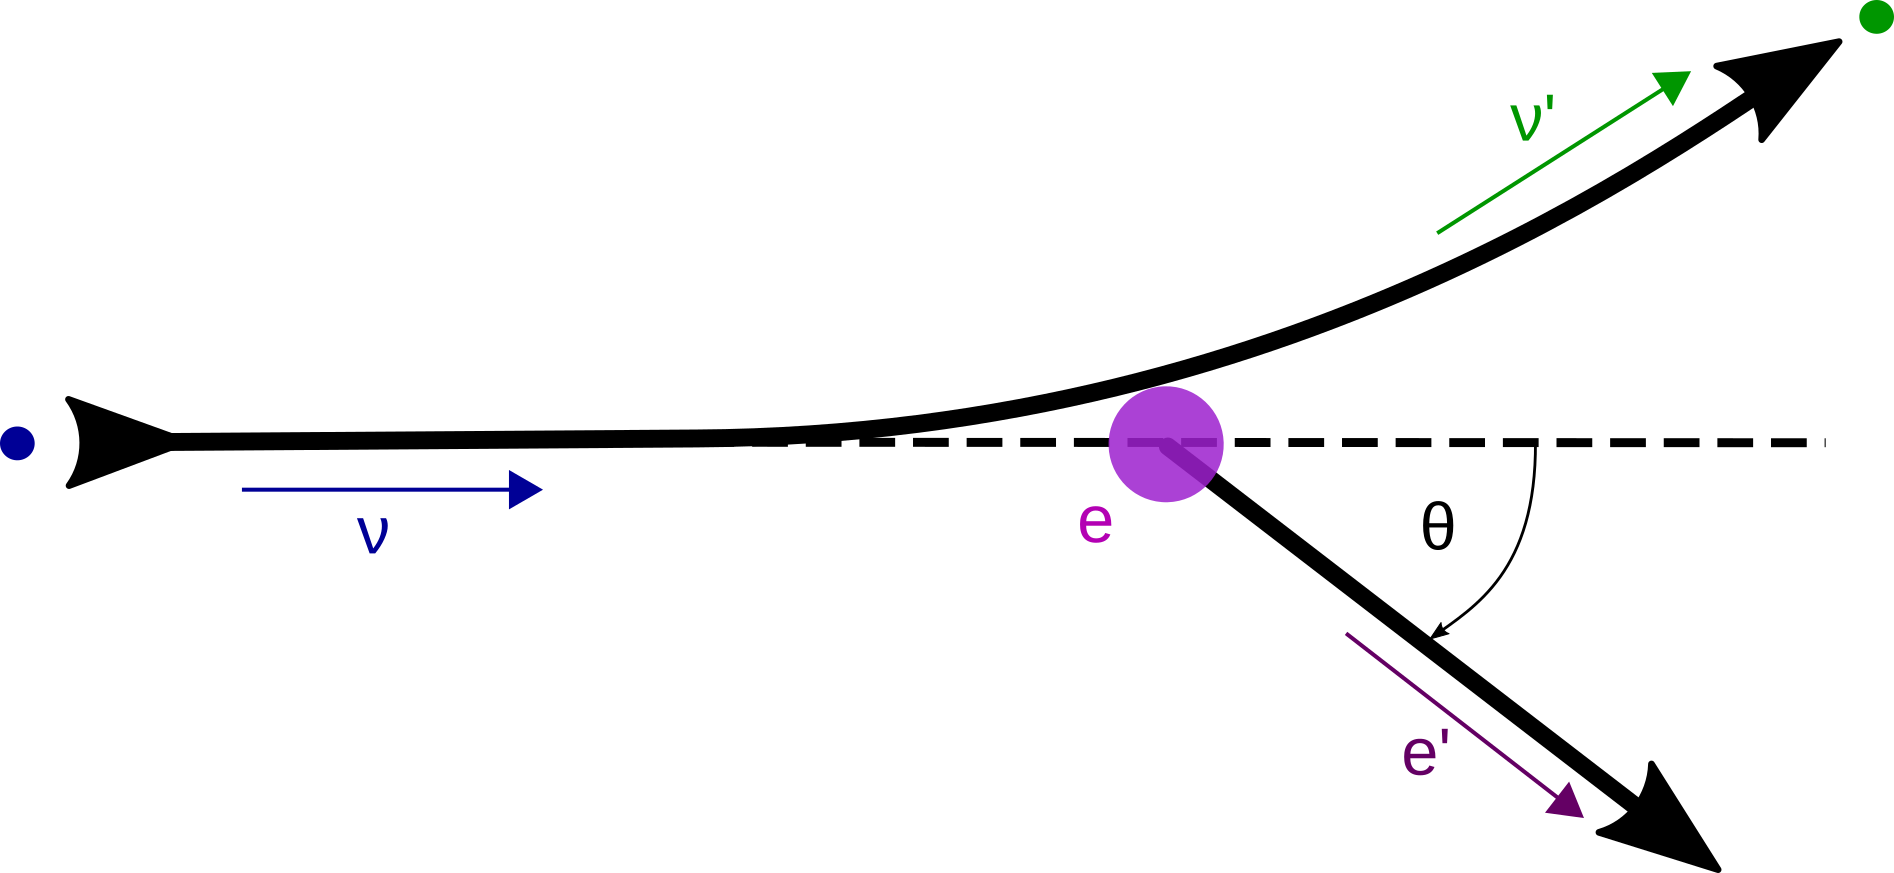
\includegraphics[width=0.55\linewidth]{Plots/NuMM/NuoneInteraction.png}
\caption{Neutrino-on-electron elastic scattering diagram}
\label{fig:NuoneDiagram}
\end{figure}

\note{Is this derivation too trivial to mention in a thesis? Should I just mention the results? I wanted to have this in the technote, but probably too detailed for a thesis...}
\todo{Also change all we to passive voice - or should I keep we here?}
From simple $2\rightarrow 2$ kinematics we can calculate
\begin{equation}
\left(P_{\nu}-P_{e^{\prime}}\right)^2=\left(P_{\nu^{\prime}}-P_e\right)^2,
\end{equation}
\begin{equation}
m_{\nu}^2+m_e^2-2E_{\nu}E_{e^{\prime}}+2E_{\nu}p_{e^{\prime}}\cos\theta=m_{\nu}^2+m_e^2-2E_{\nu^{\prime}}m_e.
\end{equation}
Using the energy conservation
\begin{equation}
E_{\nu}+m_e=E_{\nu^{\prime}}+E_{e^{\prime}}=E_{\nu^{\prime}}+T_e+m_e\Rightarrow E_{\nu^{\prime}}=E_{\nu}-T_e
\end{equation}
we get
\begin{equation}
E_{\nu}p_{e^{\prime}}\cos\theta=E_{\nu}E_{e^{\prime}}-E_{\nu^{\prime}}m_e=E_{\nu}\left(T_e+m_e\right)-\left(E_{\nu}-T_e\right)m_e=T_e\left(E_{\nu}+m_e\right),
\end{equation}
\begin{equation}
\cos\theta=\frac{E_{\nu}+m_e}{E_{\nu}}\sqrt{\frac{T_e^2}{E_{e^{\prime}}^2-m_e^2}}=\frac{E_{\nu}+m_e}{E_{\nu}}\sqrt{\frac{T_e^2}{T_e^2+2T_em_e}}.
\end{equation}
And finally we get
\begin{equation}\label{eq:ThetaTRelation}
\cos\theta=\frac{E_{\nu}+m_e}{E_{\nu}}\sqrt{\frac{T_e}{T_e+2m_e}}.
\end{equation}

We can rearrange the Eq.~\ref{eq:ThetaTRelation} to get
\begin{equation}\label{eq:TThetaRelation}
T_e=\frac{2m_eE_\nu^2\cos^2\theta}{\left(E_\nu+m_e\right)^2-E_\nu^2\cos^2\theta}.
\end{equation}
Electron's kinetic energy is therefore kinematically constrained by the energy conservation as
\begin{equation}
T_e\leq\frac{2E_{\nu}^2}{2E_{\nu}+m_e},
\end{equation}
which corresponds to the $\cos\theta\rightarrow 1$ when the recoil electron goes exactly forward in the incident neutrino direction.

Considering $E_{\nu}\sim\textsf{GeV}$, we can approximate $\frac{m_e^2}{E_{\nu}^2}\rightarrow 0$ and from Fig.\ref{fig:TThetaDistribution} we can see that we can approximate all recoil angles to be very small, therefore $\theta^2\cong \left(1-\cos^2\theta\right)$. Using Eq.\ref{eq:ThetaTRelation} we get
\begin{equation}
T_e\theta^2\cong T_e\left(1-\left(\frac{E_\nu+m_e}{E_\nu}\right)^2\frac{T_e}{T_e+2m_e}\right)
=T_e\left(1-\left(1+\frac{2m_e}{E_\nu}\right)\frac{T_e}{T_e+2m_e}\right),
\end{equation}
therefore
\begin{equation}
T_e\theta^2\cong \frac{2m_eT_e}{T_e+2m_e}\left(1-\frac{T_e}{E_\nu}\right)=2m_e\left(\frac{1}{1+\frac{2m_e}{T_e}}\right)\left(1-\frac{T_e}{E_\nu}\right),
\end{equation}
and finally
\begin{equation}\label{eqTThetaSqExp}
T_e\theta^2\cong 2m_e\left(1-\frac{T_e}{E_{\nu}}\right)<2m_e.
\end{equation}

This is a strong limit that clearly distinguishes the \gls{nuone} elastic scattering events from other similar interaction involving single electron (mainly the $\nu_e$\gls{CC} interaction).

\begin{figure}[hbtp]
\centering
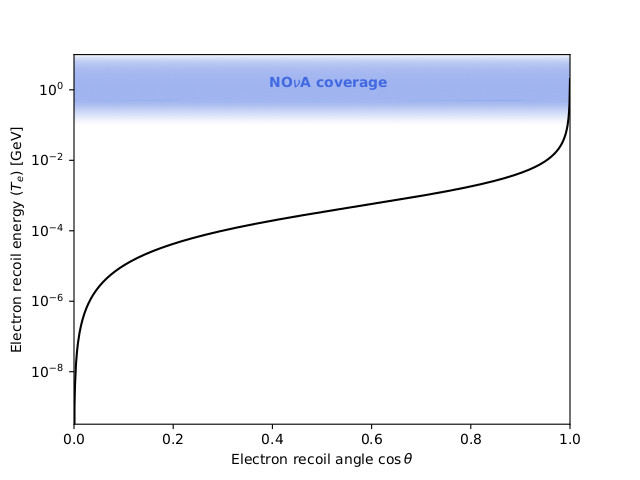
\includegraphics[width=.7\linewidth]{Plots/NuMM/KinematicsTOnTh.jpeg}
\caption[Electron recoil energy versus recoil angle]{Relation between the recoil electron's kinetic energy and angle for \acrshort{nuone} elastic scattering. The coverage of the \acrshort{NOvA} detectors for measuring the electron recoil energy is shown in blue. Only very forwards electron's are recorded in \acrshort{NOvA}.}
\label{fig:TThetaDistribution}
\end{figure}

\subsubsection{Neutrino magnetic moment cross section}
\note{Should this only be a subsubsection?}
In the ultra-relativistic limit, the neutrino magnetic moment changes the neutrino helicity, turning active neutrinos into sterile \todo{cite this properly}. Since the \gls{SM} weak interaction conserves helicity we can simply add the two contribution to the \gls{nuone} cross section incoherently \cite{nuElmagInt2015.pdf}:
\begin{equation}
\frac{d\sigma_{\nu_le^-}}{dT_e}=\left(\frac{d\sigma_{\nu_le^-}}{dT_e}\right)_{\textsf{SM}}+\left(\frac{d\sigma_{\nu_le^-}}{dT_e}\right)_{\textsf{MAG}}.
\end{equation}

The \gls{SM} contribution can be expressed as \cite{nuElmagInt2015.pdf}:
\begin{multline}
\left(\frac{d\sigma_{\nu_le^-}}{dT_e}\right)_{\textsf{SM}}=\frac{G_F^2m_e}{2\pi}\left\lbrace\left(g_V^{\nu_l}+g_A^{\nu_l}\right)^2+\left(g_V^{\nu_l}-g_A^{\nu_l}\right)^2\left(1-\frac{T_e}{E_{\nu}}\right)^2\right.\\
+\left.\left(\left(g_A^{\nu_l}\right)^2-\left(g_V^{\nu_l}\right)^2\right)\frac{m_eT_e}{E_{\nu}^2}\right\rbrace,
\end{multline}
where the coupling constants $g_V$ and $g_A$ are different for different neutrino flavours and for antineutrinos. Their values are:
\begin{align}
g_V^{\nu_e}&=2\sin^2\theta_W+1/2,\hspace{2.5cm} g_A^{\nu_e}=1/2,\\
g_V^{\nu_{\mu,\tau}}&=2\sin^2\theta_W-1/2,\hspace{2.25cm} g_A^{\nu_{\mu,\tau}}=-1/2.
\end{align}
For antineutrinos $g_A\rightarrow -g_A$.

\todo{Decide if this is actually useful or not}
Using Eq.~\ref{eq:TThetaRelation} it is possible to get the differential cross section for $\cos\theta$:
\begin{equation}
dT_e=\frac{4m_eE_\nu^2\left(m_e+E_\nu\right)^2}{\left[\left(m_e+E_\nu\right)^2-E_\nu^2\cos^2\theta\right]^2}\cos\theta d\cos\theta
\end{equation}
as
\begin{multline}
\left(\frac{d\sigma_{\nu_le^-}}{d\cos\theta}\right)_{\textsf{SM}}=
\frac{2G_F^2E_{\nu}^2m_e^2\cos\theta\left(E_{\nu}+m_e\right)^2}{\pi\left(\left(E_{\nu}+m_e\right)^2-E_{\nu}^2\cos^2\theta\right)^2}\\
\left\lbrace\left(g_V^{\nu_l}+g_A^{\nu_l}\right)^2+
\left(g_V^{\nu_l}-g_A^{\nu_l}\right)^2\left(1-\frac{2m_eE_{\nu}\cos^2\theta}{\left(E_{\nu}+m_e\right)^2-E_{\nu}^2\cos^2\theta}\right)^2\right.+\\
\left.\left(\left(g_A^{\nu_l}\right)^2-\left(g_V^{\nu_l}\right)^2\right)
\frac{2m_e^2\cos^2\theta}{\left(\left(E_{\nu}+m_e\right)^2-E_{\nu}^2\cos^2\theta\right)}\right\rbrace,
\end{multline}

\begin{table}{ht}
\centering
\caption{Neutrino-on-electron elastic scattering total cross sections. \todo{Move units to title and add cross sections with thresholds. Also reference this somewhere in text} from Fundamentals of neutrino Physics and Astrophysics, p.139}
\begin{tabular}{cc}
\hline
Process & Total cross section\\\hline
$\nu_e+e^-$ & $\simeq 93\times 10^{-43} E_\nu\unit{cm^2 GeV^{-1}}$\\
$\overline{\nu}_e+e^-$ & $\simeq \unit[39\times 10^{-43} E_\nu]{cm^2 GeV^{-1}}$\\
$\nu_{\mu,\tau}+e^-$ & $\simeq \unit[15\times 10^{-43} E_\nu]{cm^2 GeV^{-1}}$\\
$\overline{\nu}_{\mu,\tau}+e^-$ & $\simeq \unit[13\times 10^{-43} E_\nu]{cm^2 GeV^{-1}}$\\\hline
\end{tabular}
\end{table}

The neutrino magnetic moment contribution is \todo{include derivation from \cite{NeutrinoElmagFormFactors1989.pdf}} \cite{nuElmagInt2015.pdf}:
\begin{equation}
\left(\frac{d\sigma_{\nu_le^-}}{dT_e}\right)_{\textsf{MAG}}=\frac{\pi\alpha^2}{m_e^2}\left(\frac{1}{T_e}-\frac{1}{E_{\nu}}\right)\left(\frac{\mu_{\nu_l}}{\mu_B}\right)^2,
\end{equation}
where $\alpha$ is the fine structure constant \todo{Calculate the total mag moment cross sections}.

Comparison of the \gls{SM} and the neutrino magnetic moment cross sections is shown on Fig.\ref{fig:NuMMCrossSectionComparison}. Whereas the \gls{SM} cross section is flat with $T_e\rightarrow 0$, the neutrino magnetic moment cross section keeps increasing to infinity. However, this reach is limited by the experimental capabilities of detecting such low energetic neutrinos. Possible \gls{NOvA} coverage is shown in a shaded blue and it is uncertain we could actually reach as low as $100\ \unit{MeV}$ \todo{Change this claims a little bit}.

\begin{figure}[hbtp]
\centering
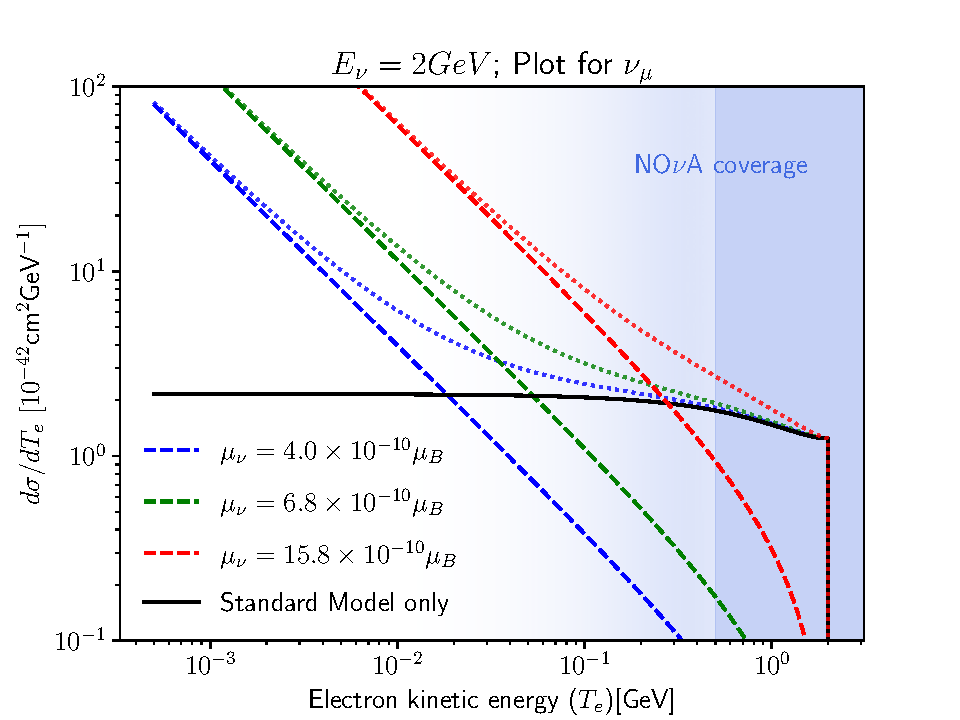
\includegraphics[width=.9\textwidth]{Plots/NuMM/dSdTNumuMMCompAltLim.pdf}
\caption[Comparison of the neutrino magnetic moment and Standard Model cross sections]{Comparison of the neutrino magnetic moment (coloured) and the \acrshort{SM} (black) cross sections for the \acrshort{nuone} elastic scattering. Different colours depict different values of the neutrino magnetic moment. Dashed lines are the individual cross sections and dotted lines are the added total cross section with the standard model contribution. \acrshort{NOvA} coverage of electron recoil energies is shown in shaded blue \todo{Reference the colours on the figures to the origins of the values (LSND and Biao)}.}
\label{fig:NuMMCrossSectionComparison}
\end{figure}

As can be seen in Fig.~\ref{fig:NuMMCrossSectionComparison} and Fig.~\ref{fig:NuMMCrossSectionRatios}, the magnetic moment contribution exceeds the \gls{SM} contribution for low enough $T_e$. This can be approximated as \cite{nuElmagInt2015.pdf}:
\begin{equation}
T_e\lesssim\frac{\pi^2\alpha^2}{G_F^2m_e^3}\left(\frac{\mu_{\nu}}{\mu_B}\right)^2\simeq 2.9\times 10^{19}\left(\frac{\mu_{\nu}}{\mu_B}\right)^2\left[\textsf{MeV}\right],
\end{equation}
which does not depend on the neutrino energy and makes experiments sensitive to lower energetic electrons more sensitive to the neutrino magnetic moment. This is especially true for the recent dark matter experiments which put stringent limits on the solar neutrino effective magnetic moment, as described in the following section.

\begin{figure}[hbtp]
\centering
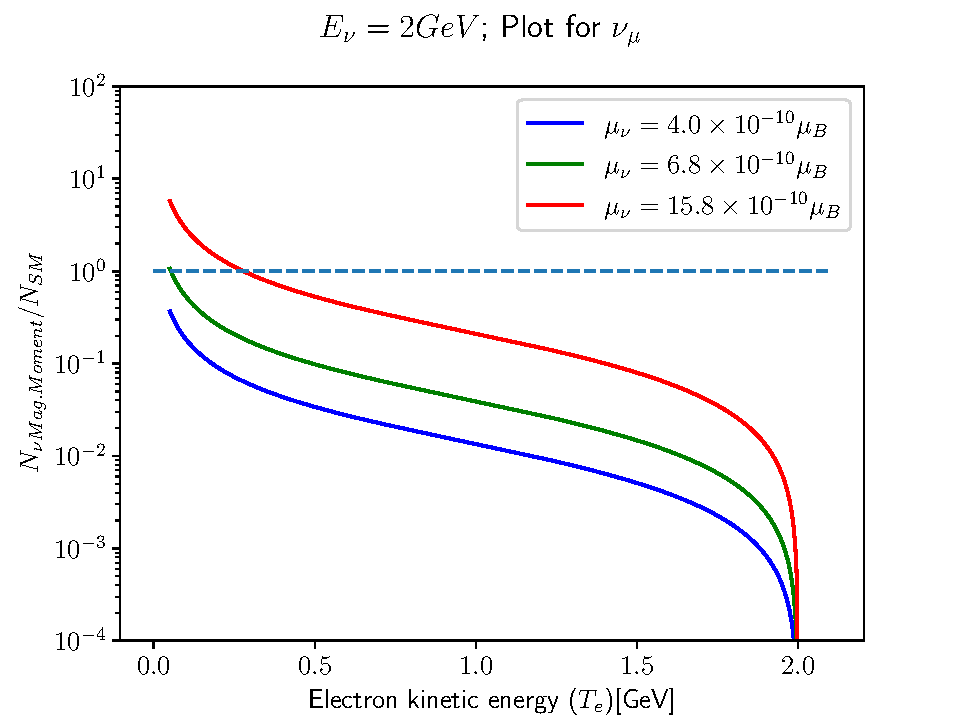
\includegraphics[width=.9\textwidth]{Plots/NuMM/RatioNumuMMCompLinX.pdf}
\caption[Ratio of the neutrino magnetic moment and Standard Model cross sections]{Ratio of the neutrino magnetic moment cross section to the \acrshort{SM} cross section for the \acrshort{nuone} elastic scattering. Different colours depict different effective muon neutrino magnetic moment values.}
\label{fig:NuMMCrossSectionRatios}
\end{figure}

%%% End of theoretical overview
%%%%%%%%%%%%%%%%%%%%%%%%%%%%%%%%%%%%%%%%%%%%%%%%%%%%%%%%%%%%%%%%%%%%%%%%%%%%%%%

\section{Experimental overview}
\note{Should I include cosmological implication here?}
\todo{Describe the limits from other experiments}
%%%%%%%%%%%%%%%%%%%%%%%%%%%%%%%%%%%%%%%%%%%%%%%%%%%%%%%%%%%%%%%%%%%%%
%%%                       ANALYSIS OVERVIEW                       %%%
%%%%%%%%%%%%%%%%%%%%%%%%%%%%%%%%%%%%%%%%%%%%%%%%%%%%%%%%%%%%%%%%%%%%%
\section{Analysis overview}
In this analysis we are searching for a signal of possible neutrino magnetic moment events in the \gls{NOvA} \gls{ND}. This signal would manifest as an excess of \gls{nuone} elastic scattering events at low electron recoil energies on top of the \gls{SM} background, as described in Sec.~\ref{sec:MeasuringNuMM}. In case we would not observe any excess (null hypothesis), we would provide an upper limit on the effective muon neutrino magnetic moment.

The \gls{nuone} interactions are also used in the \gls{ND} group's analysis to constraint the neutrino beam prediction \cite{NOVA-doc-56383}, which relies on the precise theoretical knowledge of the \gls{nuone} interaction cross section. They compare the total number of recorded \gls{nuone} interactions, with background subtracted based on a comparison of data and simulation in a sideband region, to the prediction. Since the number of \gls{nuone} events should only depend on the normalization of the neutrino beam, this analysis should give us a precise validation, or correction, of the neutrino flux normalization. There has been a large amount of work going into this analysis, including making special samples, weights, event classifiers, developing a dedicated event selection, or developing a background subtraction method, among others. To save time and analysis effort, we have taken most of these work at face value and applied it to the neutrino magnetic moment analysis. This will help us get the first good estimate of \gls{NOvA}'s capabilities to constraint (or measure) the neutrino magnetic moment.

The same detector signature of a single forward going electron shower, as present in the \gls{nuone} events, is also present in the \gls{LDM} analysis \cite{NOVA-doc-59439}. This analysis is using a similar event selection to select the \gls{LDM} events as the \gls{ND} group, only without the final $E\theta^2$ cut (see Sec.\ref{sec:EventSelection}). However, instead of simply comparing the total event counts, the \gls{LDM} analysis is using a CAFAna-based fitting framework to fit for the possible \gls{LDM} signal in a distribution of electron recoil energy multiplied by electron recoil angle squared.

%What are we trying to achieve? We are trying to see the low energy excess of very forward neutrino-on-electron ($\nu$-on-e) events. We can either do this via a counting experiment (possibly with various control samples/regions to control backgrounds and systematics), or with a fit to the energy spectrum of well-selected $\nu$-on-electron events.

Our analysis strategy is to compare the recorded number of neutrino events in data with a predicted number of signal events, which depends on the neutrino magnetic moment value, on top of a \gls{SM} background. We use the \gls{ND} group's sideband region to constraint the non-\gls{nuone} background with data. It is also possible to use a second sideband sample, based on the electron recoil energy, to provide an additional constraint on the \gls{nuone} background, but this idea has not been visited yet.

In the future, this analysis can be improved for example by improving the event selection, creating additional background samples, by including antineutrino events, or by using using a fit to the energy distribution, similarly to the \gls{LDM} analysis.

This section describes the simulation samples used to predict the number of signal and background events (Sec.\ref{sec:datasets}) and the weights used to correct for known limitations of the simulation (Sec. \ref{sec:anaWeights}).

% Not sure if this should be here or in the datasets subsection... Here on forward I'm going to describe the differences between these (definitions, weights, signal def, systematics. What is the same: event selection and binning. They're joint together in the fitting framework, where the $\nu_e$CC MEC and the other backgrounds are simply summed together and scaled together. The $\nu$-on-e background (also called the irreducible background by the LDM analysis) is treated/scaled separately.

\subsection{Datasets and Event Reconstruction details}\label{sec:datasets}
For this analysis we are using near detector CAF samples with the standard Production 5.1 reconstruction.

We are following the standard data blinding procedure and have not looked at any data events until the analysis passes the full collaboration review. The Near Detector group has validated \todo{Figure out where did Yiwen and Wenjie actually look at the data} using this data sample.

The exposure of the data sample is approximately $1.3848600\times 10^{21}\ \unit{POT}$. This is the exposure we use for all the following studies shown in this technical note.
The Prod5.1 ND data sample contains data from run 10391 in epoch1a (2014-08-22 21:08:40) until run 14010 in epoch 11a (2021-02-03 15:48:21) (from the period and epoch naming wiki page https://cdcvs.fnal.gov/redmine/projects/novaart/wiki/Period\_and\_Epoch\_Naming)

\todo{Briefly describe the MC details. Versions of the individual simulation software}
To tackle the low number of \gls{nuone} and $\nu_e$\gls{CC} \gls{MEC} events in the nominal simulation sample we are using a suit of nominal and enhanced simulation samples for four different signal and background components. Each one contains its nominal sample and special systematically shifted samples for the detector systematics. The use of the samples is summarised in table \ref{tab:SignalDefinitions} and described in detail below.

The \textsf{GENIE} tune is \texttt{GENIE N1810j 02 11a} (from the Prod5.Frankenstein docdb: 53360).
The Genie release used for this production is R20-08-06-prod5.1genie.h, which has GENIE version V3.0.6 \cite{GENIE}

Also prod5.1 uses Geant4 v4.10.4.p02 \cite{Geant4}

We use the standard NOvA simulation (reference NOvA 3fl paper DOI: 10.1103/PhysRevD.106.032004)

Describe how did we deal with the GENIE skew fix. It was the GSF weights that forces "us" to treat the nueCC MEC background differently than the other background. As I understand it, the GSF is applied simply as the new weight. No change to the systematics is required.

Reference: A. Mislivic, “Genie skew reweight validation.” NOvA Internal Document, DocDB: 553811
[from antinueCC IncXSec docdb:53691]
"Final state kinematics were predicted by the N1810j 00 000 tune, but total cross section were generated with the intended N1810j 0211a179 tune, which differed in RES and DIS rates tuned to external data. Properly correcting the skew180 would require all simulation to be regenerated, so a temporary solution developed by the NOvA181 Cross-section Tuning Group involves reweighing production 5.1 events to the default N1810j 00 000.182 An additional modification to the GENIE MEC contribution are applied to better agree with NOvA183 ND data.

MC includes simulation in the rock surrounding the ND

\todo{Describe here that we're using the nominal ND MC sample for signal utilizing the simple relationship between the Standard Model cross section and the neutrino magnetic moment cross section (ref. theory)}

The signal of the neutrino magnetic moment analysis is just a re-weighted signal of the \gls{nuone} analysis from the near detector group. We are using the same event selection as the near detector group.

\todo{Say already here that the POT inside the enhanced MC samples are not properly accounted for in CAFAna (Loader issue) and so the event counts need to be adjusted post-hoc}

\begin{table}[!ht]
\centering
\caption{Overview of the simulation samples corresponding to different signal and background components.}
\def\arraystretch{1.4}
\begin{tabular}{l@{\hskip 1in}l}
Signal                   & Enhanced $\nu$-on-e sample\\
$\nu$-on-e background    & Enhanced $\nu$-on-e sample\\
$\nu_e$CC MEC background & Enhanced $\nu_e$CC MEC sample\\
Other background         & Nominal ND CAF sample
\end{tabular}
\label{tab:DefinitionsOverview}
\end{table}

\subsubsection*{Enhanced $\nu$-on-e sample}
\todo{Describe the nuone sample}
Created by Wenjie Wu (was it just him or also Yiwen?) to do ... and fully described in the technote \cite{NOVA-doc-56383}. Using the overlayed and filematched samples for consistency.

Incorrect POT is 3.6995434e+20, Correct POT is 1.7209423e+24 (this should be filematched)

\todo{Find a reference and reasoning for why Wenjie hasn't created the other systematics samples}
We only have the selected few systematics definitions because ... 

\todo{Describe the differences}
\begin{itemize}
\item Missing cross section parameters - unable to use cross section weights or so
\item Special mode for nu-on-e elastic scattering 10005
\end{itemize}

\subsubsection*{Enhanced $\nu_e$CC MEC sample}
Created by Yiwen Xiao \cite{NOVA-doc-56383} to tackle the low statistics of the $\nu_e$CC MEC background events and subsequently large and unphysical cross section weights.

Incorrect POT is 4.7334120e+23 and correct POT is 1.9880340e+24. This is filematched

\todo{List the limitations of the sample in the q3-q0 parameter space}

\subsubsection*{Near Detector filematched CAF sample}
\todo{describe all the ND nominal CAF samples}
\todo{Also mention the decaf sample and discuss if we could use them or not}

The nominal ND MC includes 4x data POT. The systematics are file-matched to remove any statistical bias

Total POT is 5.54497e+21
But for the filematched samples (batch 2) there's only 1.93109e+21

\subsection{Analysis weights}\label{sec:anaWeights}
\todo{Describe why do we use weights}
What are the weights we are using and why?

To correct for known deficiencies in simulation of neutrino flux or cross sections we apply weights calculated for each event.

Table \ref{tab:WeightsOverview} shows what CAFAna weights are used to simulate what signal/background sample.

\begin{table}[!ht]
\centering
\caption{Overview of CAFAna weights applied to each analysis sample.}
\def\arraystretch{1.4}
\begin{tabular}{l@{\hskip 1in}l}
Signal                   & Flux and neutrino magnetic moment weights\\
$\nu$-on-e background    & Flux and radiative correction weights\\
$\nu_e$CC MEC background & Flux and cross section weights\\
Other background         & Flux and cross section weights
\end{tabular}
\label{tab:WeightsOverview}
\end{table}

\subsubsection*{PPFX weight}
\texttt{ana::kPPFXFluxCVWgt} \cite{NOVA-doc-23441}
\todo{What does this do (one sentence ish).}
Maybe cite Leo's thesis? Or paper?
L. Aliaga, “Neutrino Flux Prediction for the NuMI Beamline.” PhD Thesis, FERMILAB-1081
THESIS-2016-03


\subsubsection*{Prod5.1 GSF XSec weight}
\texttt{ana::kXSecCVWgt2020GSFProd51}
\todo{Find the reference: possibly Maria's docdb:53336 together with the official 2020 XSec tuning technote docdb:43962.}

NOvAReweight reference: J. Wolcott, “NOvARwgt software.” https://github.com/novaexperiment/NOvARwgt-public.

\todo{Briefly describe what does this do. Also mention Yiwen's talk/technote about the large XSec weights that made her create an enhanced nueCC MEC sample.}

We are only using the for the background since we assume that the cross section for the signal is perfect. Also there are not weights for this kind of interaction.

\subsubsection*{Radiative correction weight}
\todo{Why are we doing this? (reference Yiwen's talk/technote).}

Mention here where did I get the original GENIE cross section from (reference Yiwen's talk or technote, plus the original paper that was used). nu-on-e technote\cite{NOVA-doc-56383}

\todo{Write out the actual version of the weight. Including the original and the corrected XSec constants}

MINERvA paper:
https://journals.aps.org/prd/pdf/10.1103/PhysRevD.100.092001

Say that we are not using the third part of the correction because it is tiny and it makes no difference. (tried and tested)

\todo{correct the equation}
Calculated as 
\begin{equation}
weight_{\text{Radiative Corr.}} = \left.\frac{d\sigma_{\nu-on-e}}{dy}\right|_{\text{Radiative Corr.}} / \left.\frac{\textsf{d}\sigma_{\nu-on-e}}{\textsf{d}y}\right|_{\text{GENIE 3}};\,y=\frac{E_e-m_e}{E_\nu}
\end{equation}

\subsubsection*{Neutrino magnetic moment signal as a weight}
\todo{What does this do and why does it work? Reference the theory part as to why is the magnetic moment signal simply a rescaling of the GENIE cross section.}

Using the same tree-level cross section from GENIE as in the rad. corr. weight.

\todo{Write the name of the weight in CAFAna/nuone namespace and where it is located}

\todo{correct the equation}
Calculated as 
\begin{equation}
weight_{\nu\text{ Mag. Moment}} = \left.\frac{d\sigma_{\nu-on-e}}{dy}\right|_{\nu\text{ Mag. Moment}} / \left.\frac{\textsf{d}\sigma_{\nu-on-e}}{\textsf{d}y}\right|_{\text{GENIE 3}};\,y=\frac{E_e-m_e}{E_\nu}
\end{equation}


%%%%%%%%%%%%%%%%%%%%%%%%%%%%%%%%%%%%%%%%%%%%%%%%%%%%%%%%%%%%%%%%%%%%%
%%%                         EVENT SELECTION                       %%%
%%%%%%%%%%%%%%%%%%%%%%%%%%%%%%%%%%%%%%%%%%%%%%%%%%%%%%%%%%%%%%%%%%%%%
\section{Event selection}

We are trying to select low energy neutrino-on-electron events, which are characterised by a single very forward going electron shower. Since these are the same events as are used in the \gls{ND} group's analysis to constraint the neutrino beam prediction with a \gls{nuone} events \cite{NOVA-doc-56383}, we have taken taken their event selection without changes. This is to save time and analysis efforts, but also to get a first good estimation of \gls{NOvA}'s capabilities to constraint (or measure) neutrino magnetic moment. Almost the same selection is also used in the \gls{LDM} analysis \cite{NOVA-doc-59439}, only without the final $E\theta^2$ cut.

We explain the motivation behind each cut of the event selection and discuss their effect on the neutrino magnetic moment events below. We also consider possible improvements to the event selection for a future (re-)analysis. \todo{Also describe how were the cuts selected}

\subsubsection*{Signal Definition}
To define the signal and background samples we use the true information listed in Tab.~\ref{tab:SignalDefinitions}. The neutrino magnetic moment signal definition is the same as that for the \gls{nuone} background with the neutrino magnetic moment weight applied (explained in Sec.~\ref{sec:anaWeights}). 

The signal definitions use the \texttt{kMode} variable instead of the \texttt{kIntType}, which is now deprecated (ref.: various Slack conversations). Mode 10005 denotes only the \gls{nuone} events and is only available for the enhanced \gls{nuone} samples, while mode 5 denotes all electron scattering events, including inverse muon decay interactions. That is why we had to add a requirement of an electron in the final state. Mode 10 denotes all Meson Exchange Current (MEC) events.

We are using the \gls{ND} group's \cite{NOVA-doc-56383} signal definition including a requirement for the true vertex to lie within their fiducial volume (defined below). This is the cut name \texttt{NDNuoneFiducial}. This is in contrast with the \gls{LDM} analysis \cite{NOVA-doc-59439}, which uses the \texttt{ana::kVtxIsContained} cut instead, which has a looser boundary. This choice has only a negligible effect on the final number of selected events and only affects the selection efficiency.

\begin{table}[!ht]
\centering
\caption{Overview of signal and background definitions.}
\def\arraystretch{1.4}
\begin{tabular}{p{.25\textwidth}p{.7\textwidth}}
Signal                   & \texttt{kMode}== 10005 \&\& \texttt{NDNuoneFiducial}\\
$\nu$-on-e background    & \texttt{kMode}== 10005 \&\& \texttt{NDNuoneFiducial}\\
$\nu_e$CC MEC background & !(\texttt{kMode}== 5 \&\& \texttt{kElInFinState} \&\& \texttt{NDNuoneFiducial}) \&\& (\texttt{kIsCC} \&\& \texttt{kIsNue} \&\& \texttt{kMode == 10})\\
Other background         & !(\texttt{kMode}== 5 \&\& \texttt{kElInFinState} \&\& \texttt{NDNuoneFiducial}) \&\& !(\texttt{kIsCC} \&\& \texttt{kIsNue} \&\& \texttt{kMode} == 10)
\end{tabular}
\label{tab:SignalDefinitions}
\end{table}

\subsubsection*{Spill Quality Selection}
To ensure good data quality, we apply the following criteria on the run, subrun and spill level. 
\todo{Add a description of the spill quality cuts (only applied to data)}

\subsubsection*{Basic Reconstruction Quality Selection}

\todo{Split the pre-selection into basic reco quality and basic event selection}
Pre-selection cuts include basic quality cuts that remove events with invalid vertex reconstruction and events with no reconstructed prongs, as shown on Fig.~\ref{fig:BasicPreSelectionCuts}. In pre-selection we also include a cut on the time difference between the mean times of the "current" slice and of the slice closest in time, which should be $>25\ \unit{ns}$. This ensures that ... \todo{This is to remove slicing failures that split the two gamma from a $\pi^0$ into two slices that resemble electron signal. Should we remove them now though?}.

\begin{figure}[hbtp]
\centering
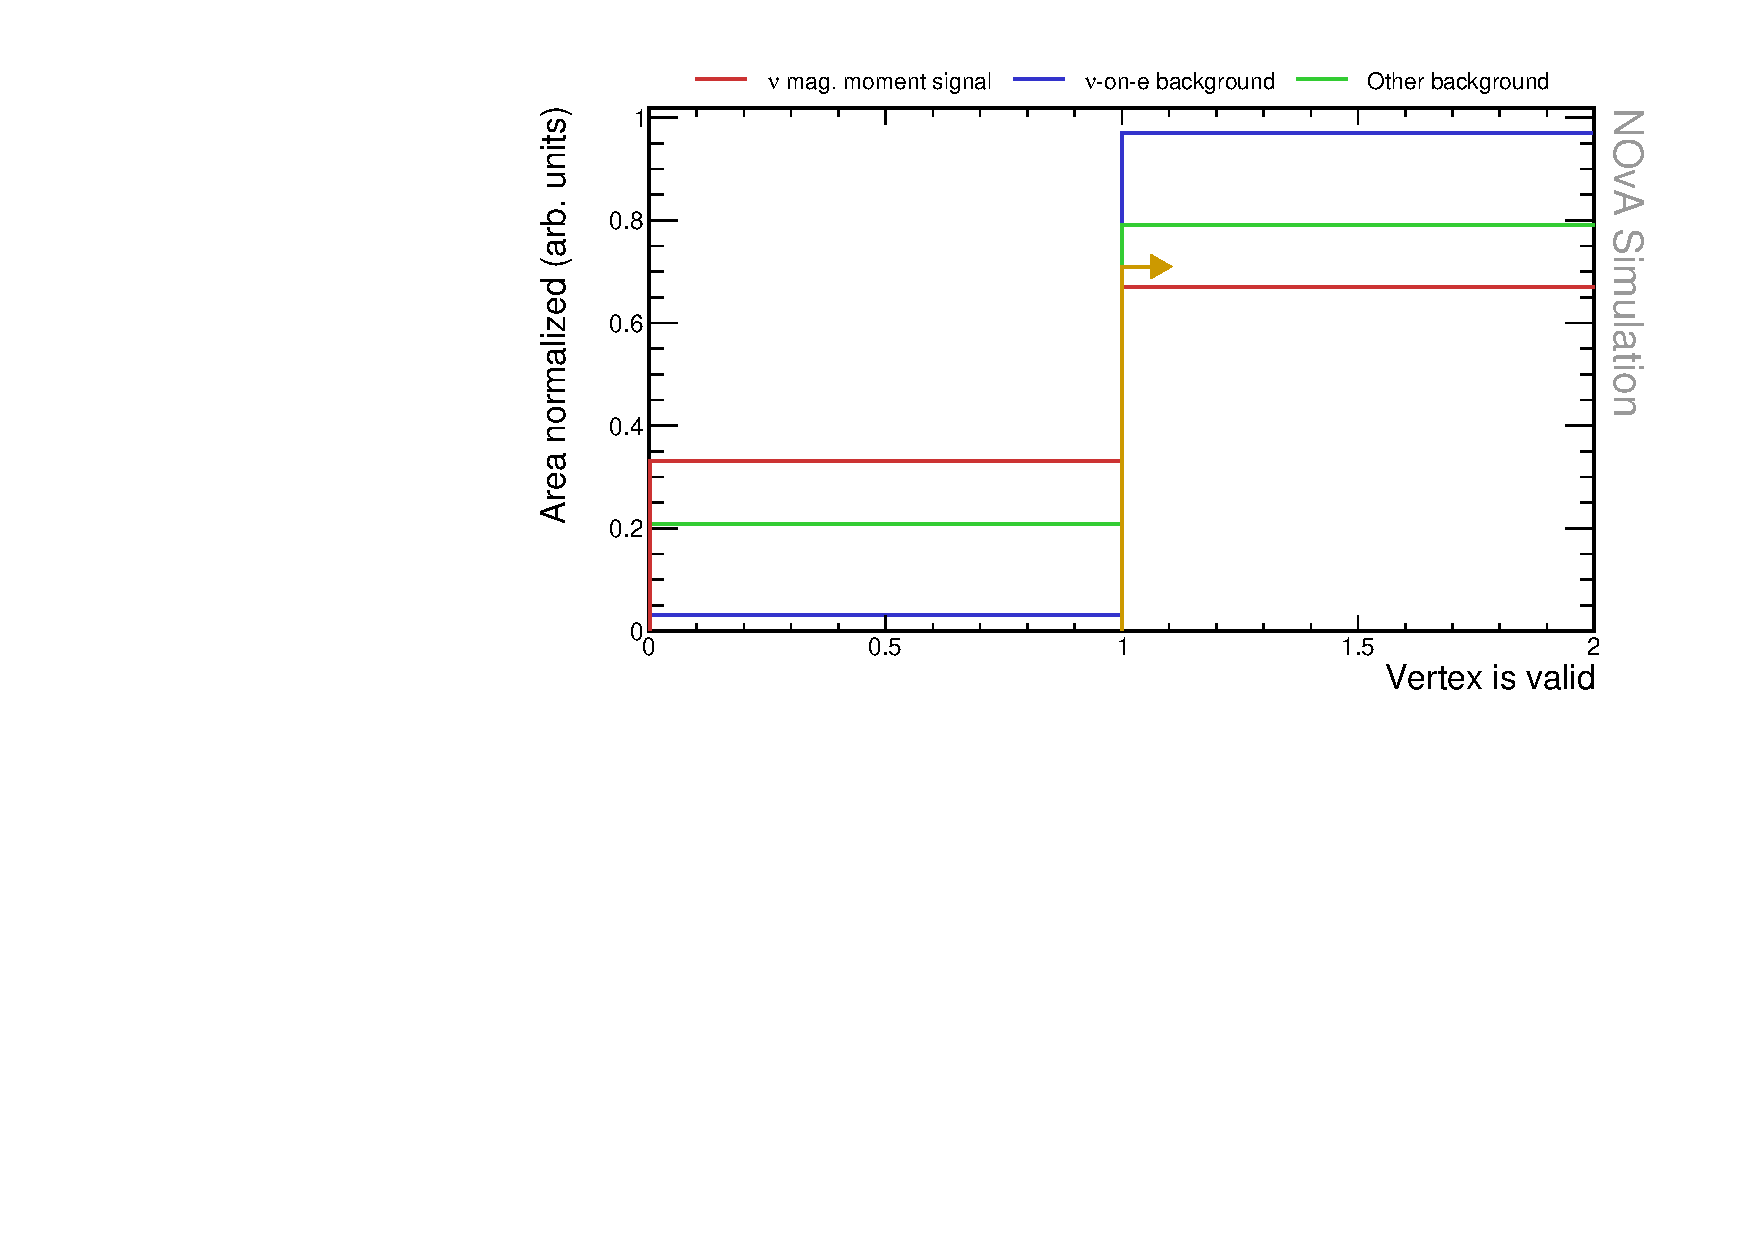
\includegraphics[width=.9\textwidth]{Plots/NuMMEventSelection/NoCut_vtxIsValid.pdf}
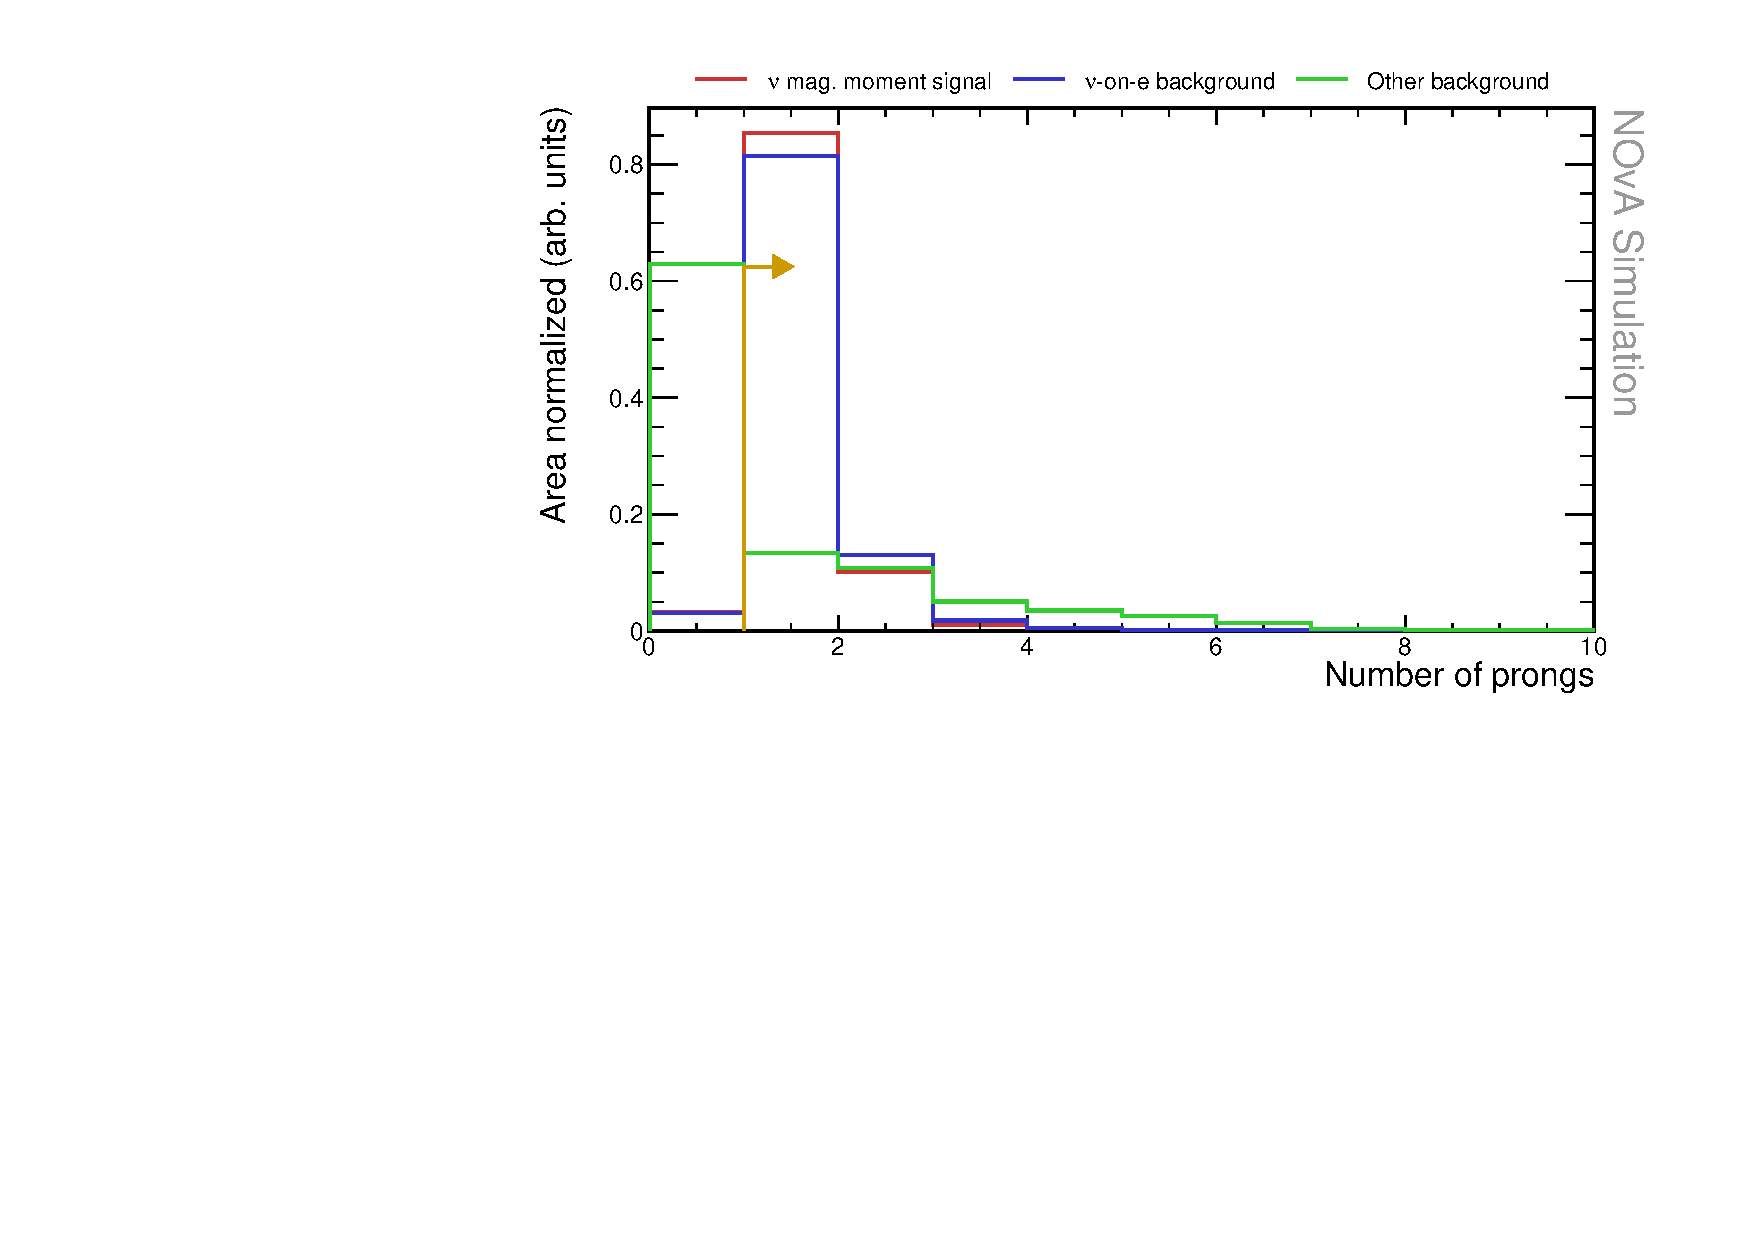
\includegraphics[width=.9\textwidth]{Plots/NuMMEventSelection/NoCut_NPng.pdf}
\caption{Relative comparison of signal, $\nu$-on-e background, and other background events for basic pre-selection variables. No cuts were applied to make these plots. Gold lines show the cut values for the shown variables.}
\label{fig:BasicPreSelectionCuts}
\end{figure}

\subsubsection*{Basic Event Selection}

The pre-selection cuts have been kept from the $\nu_e$\gls{CC} analysis with loosened cut values \todo{find a reference for this analysis}.
They also remove the obvious $\nu_\mu$CC interactions by requiring that the length of the longest prong is $<800\ \unit{cm}$, number of planes crossed by the longest prong is $<120$, and the summed number of cells for all prongs in the slice is $<600$.Relative comparison of signal, $\nu$-on-e background, and other background distributions for the pre-selection variables is shown on Fig.~\ref{fig:PreSelectionCuts}.

\begin{figure}[hbtp]
\centering
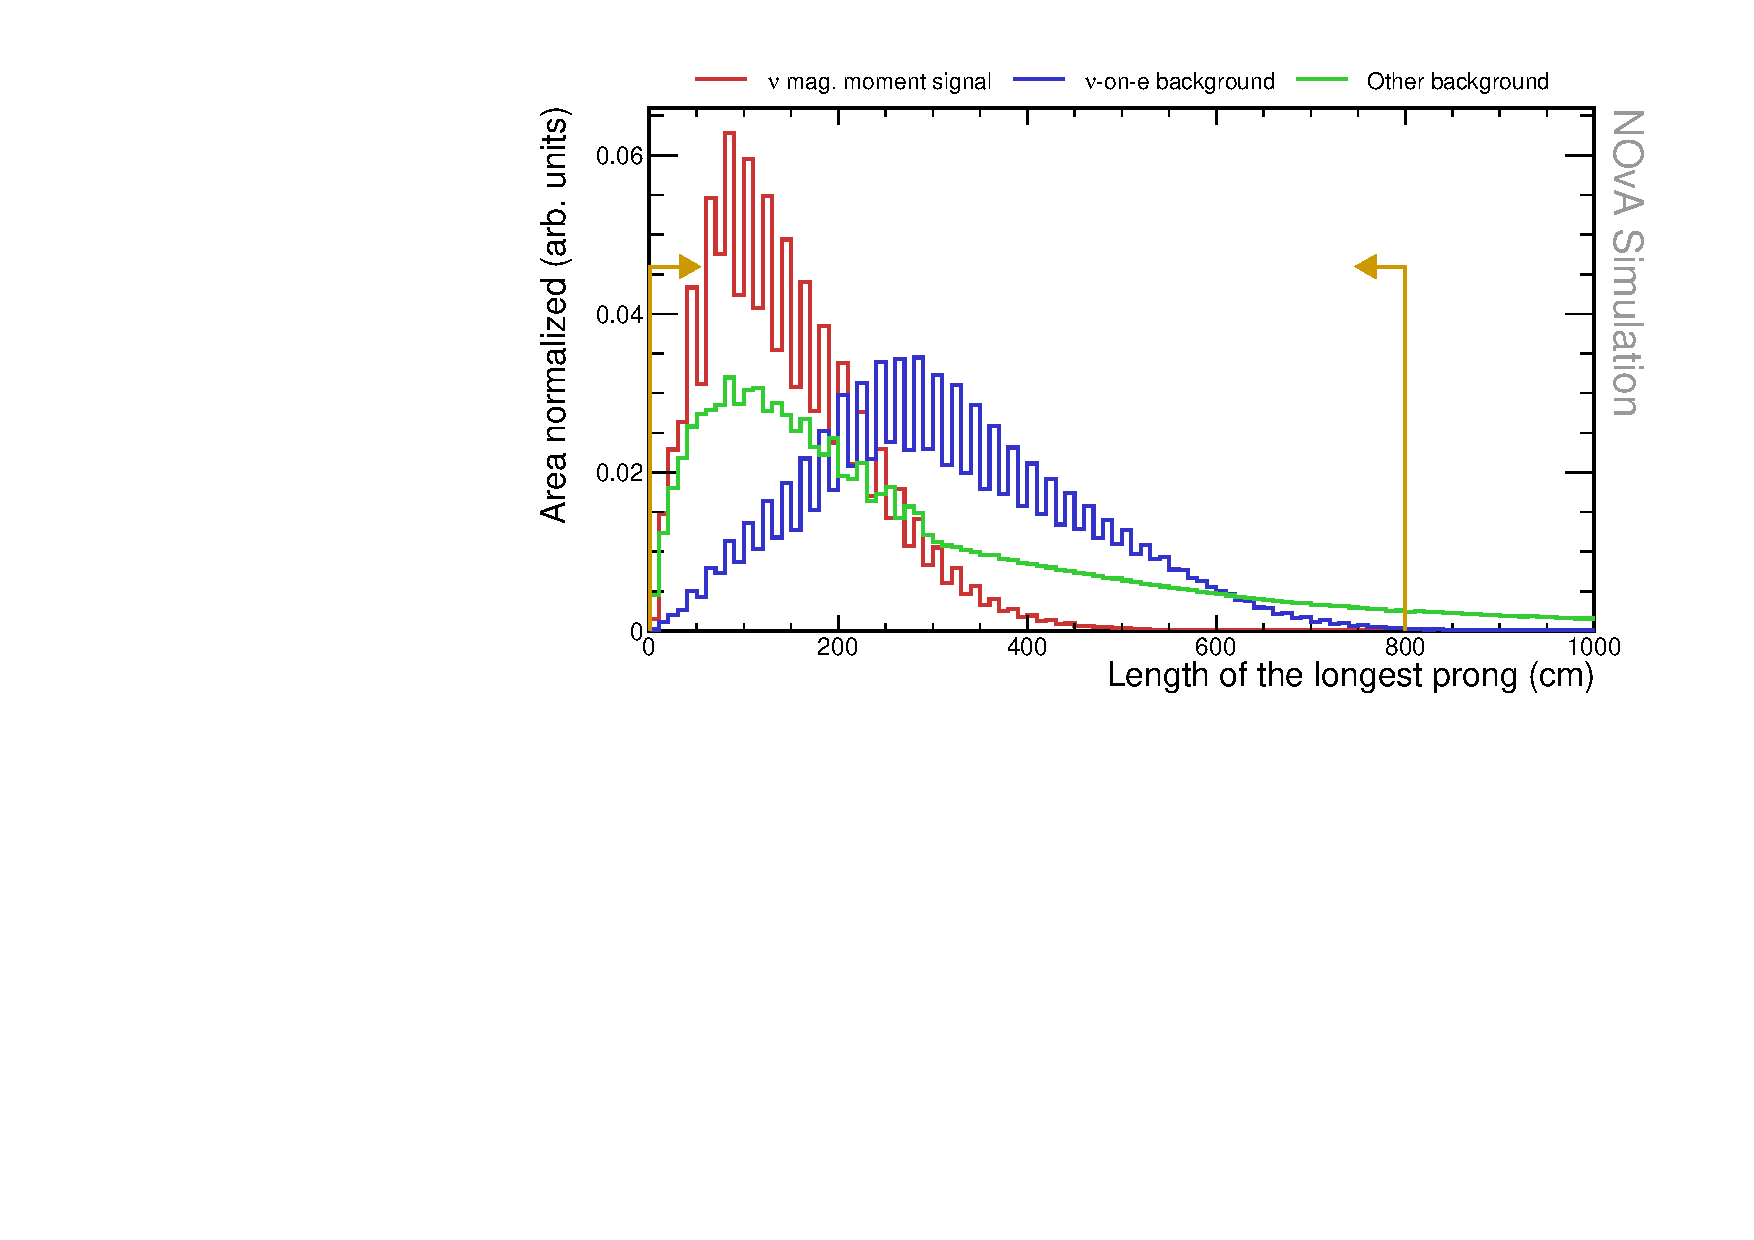
\includegraphics[width=.9\textwidth]{Plots/NuMMEventSelection/N1Cut_longestProng.pdf}
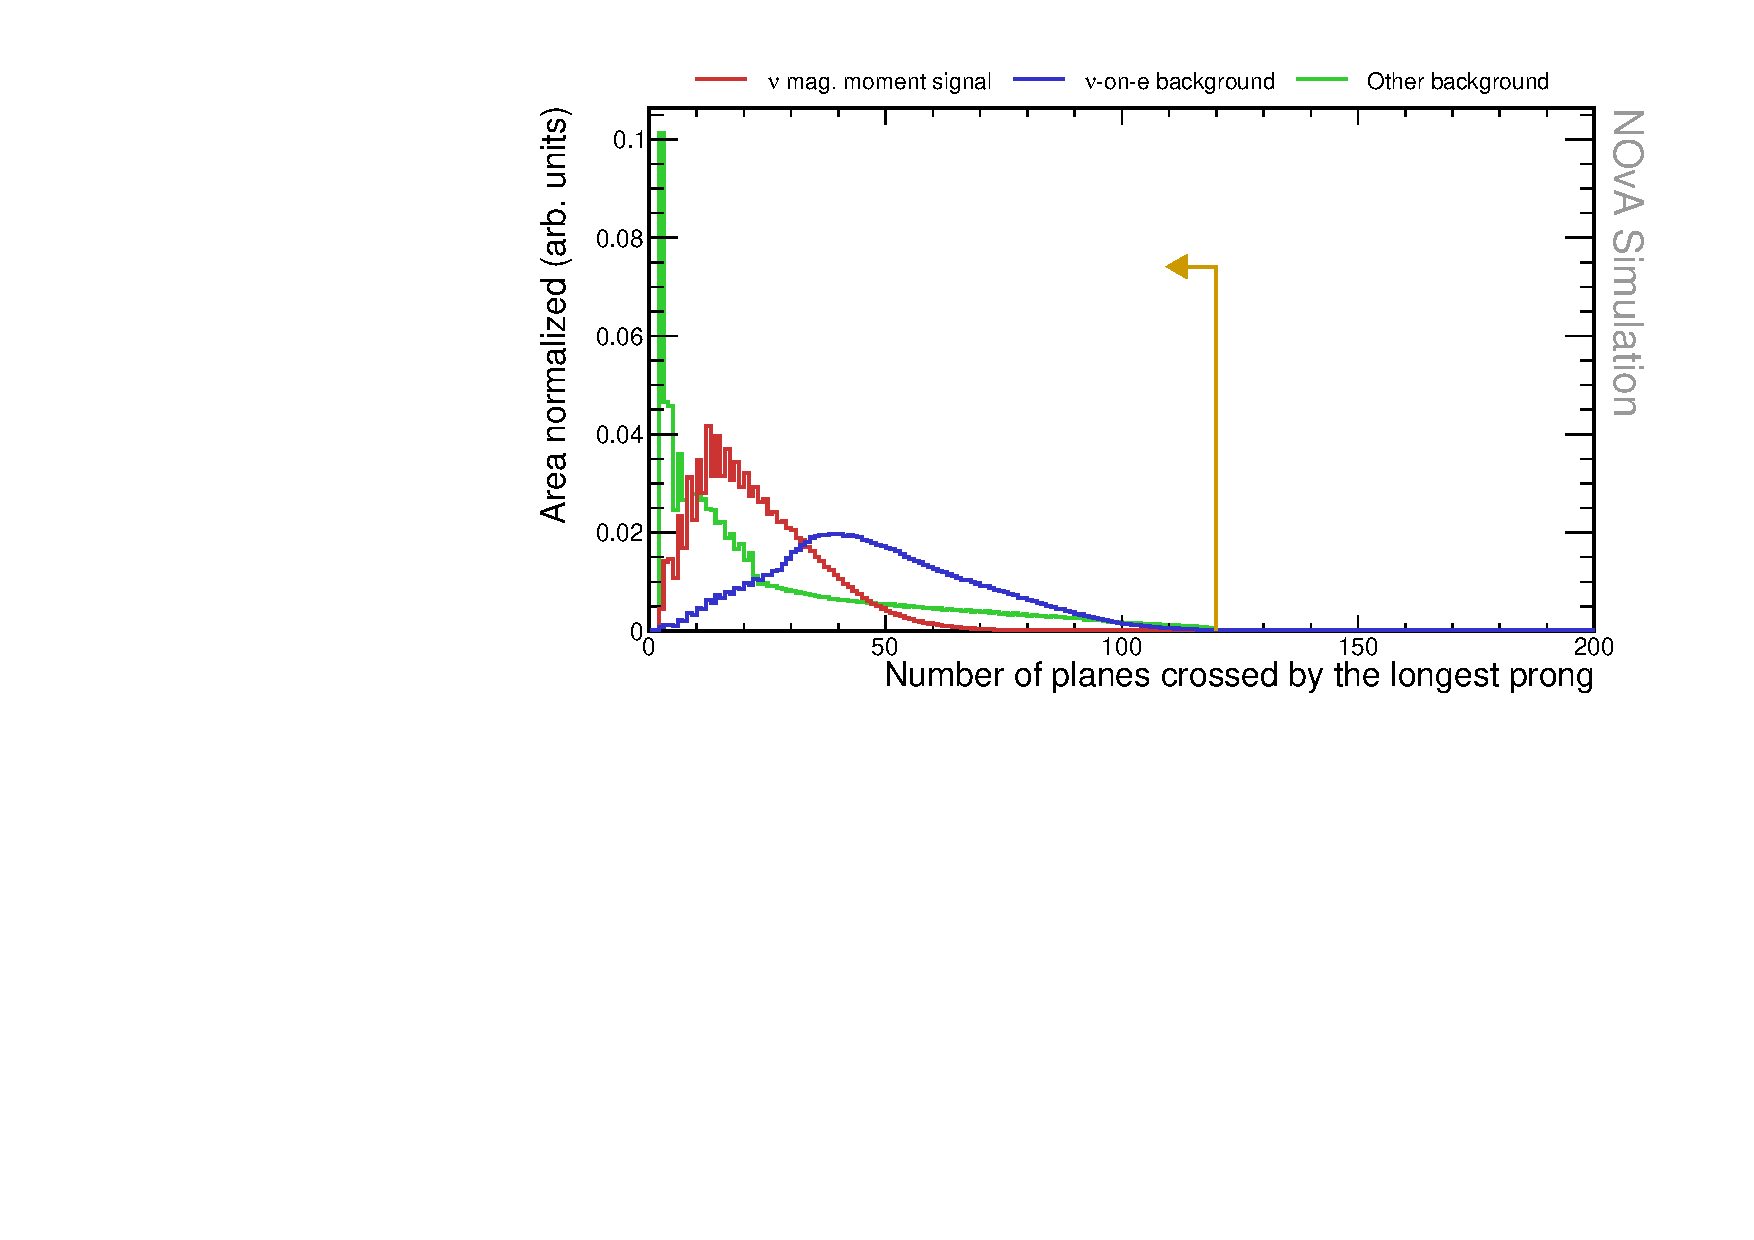
\includegraphics[width=.9\textwidth]{Plots/NuMMEventSelection/N1Cut_NPlanes.pdf}
\caption{Relative comparison of signal, $\nu$-on-e background, and other background events for pre-selection variables. Cuts on VtxIsValid and number of prongs were applied to make these plots. Gold lines show the cut values for the shown variables.}
\label{fig:PreSelectionCuts1}
\end{figure}

\begin{figure}[hbtp]
\centering
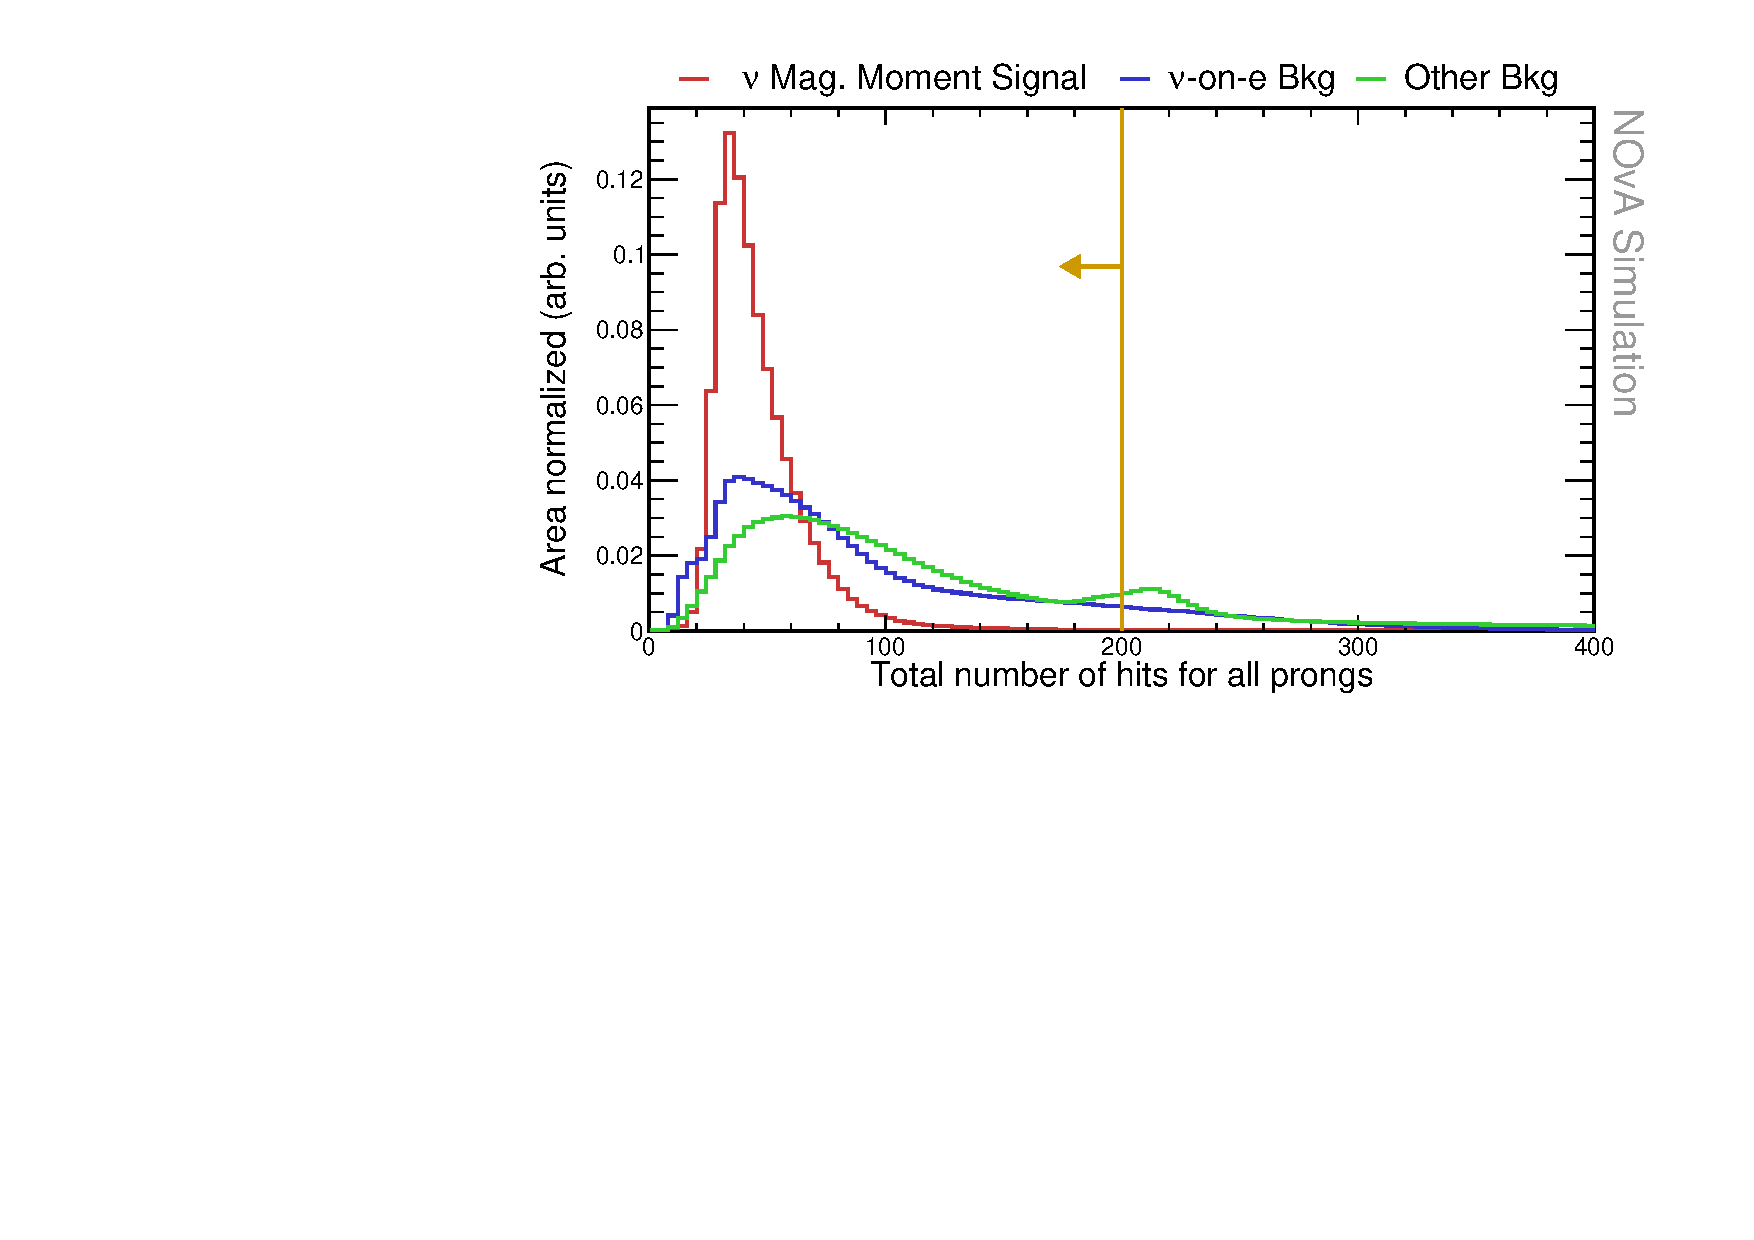
\includegraphics[width=.9\textwidth]{Plots/NuMMEventSelection/N1Cut_NHits.pdf}
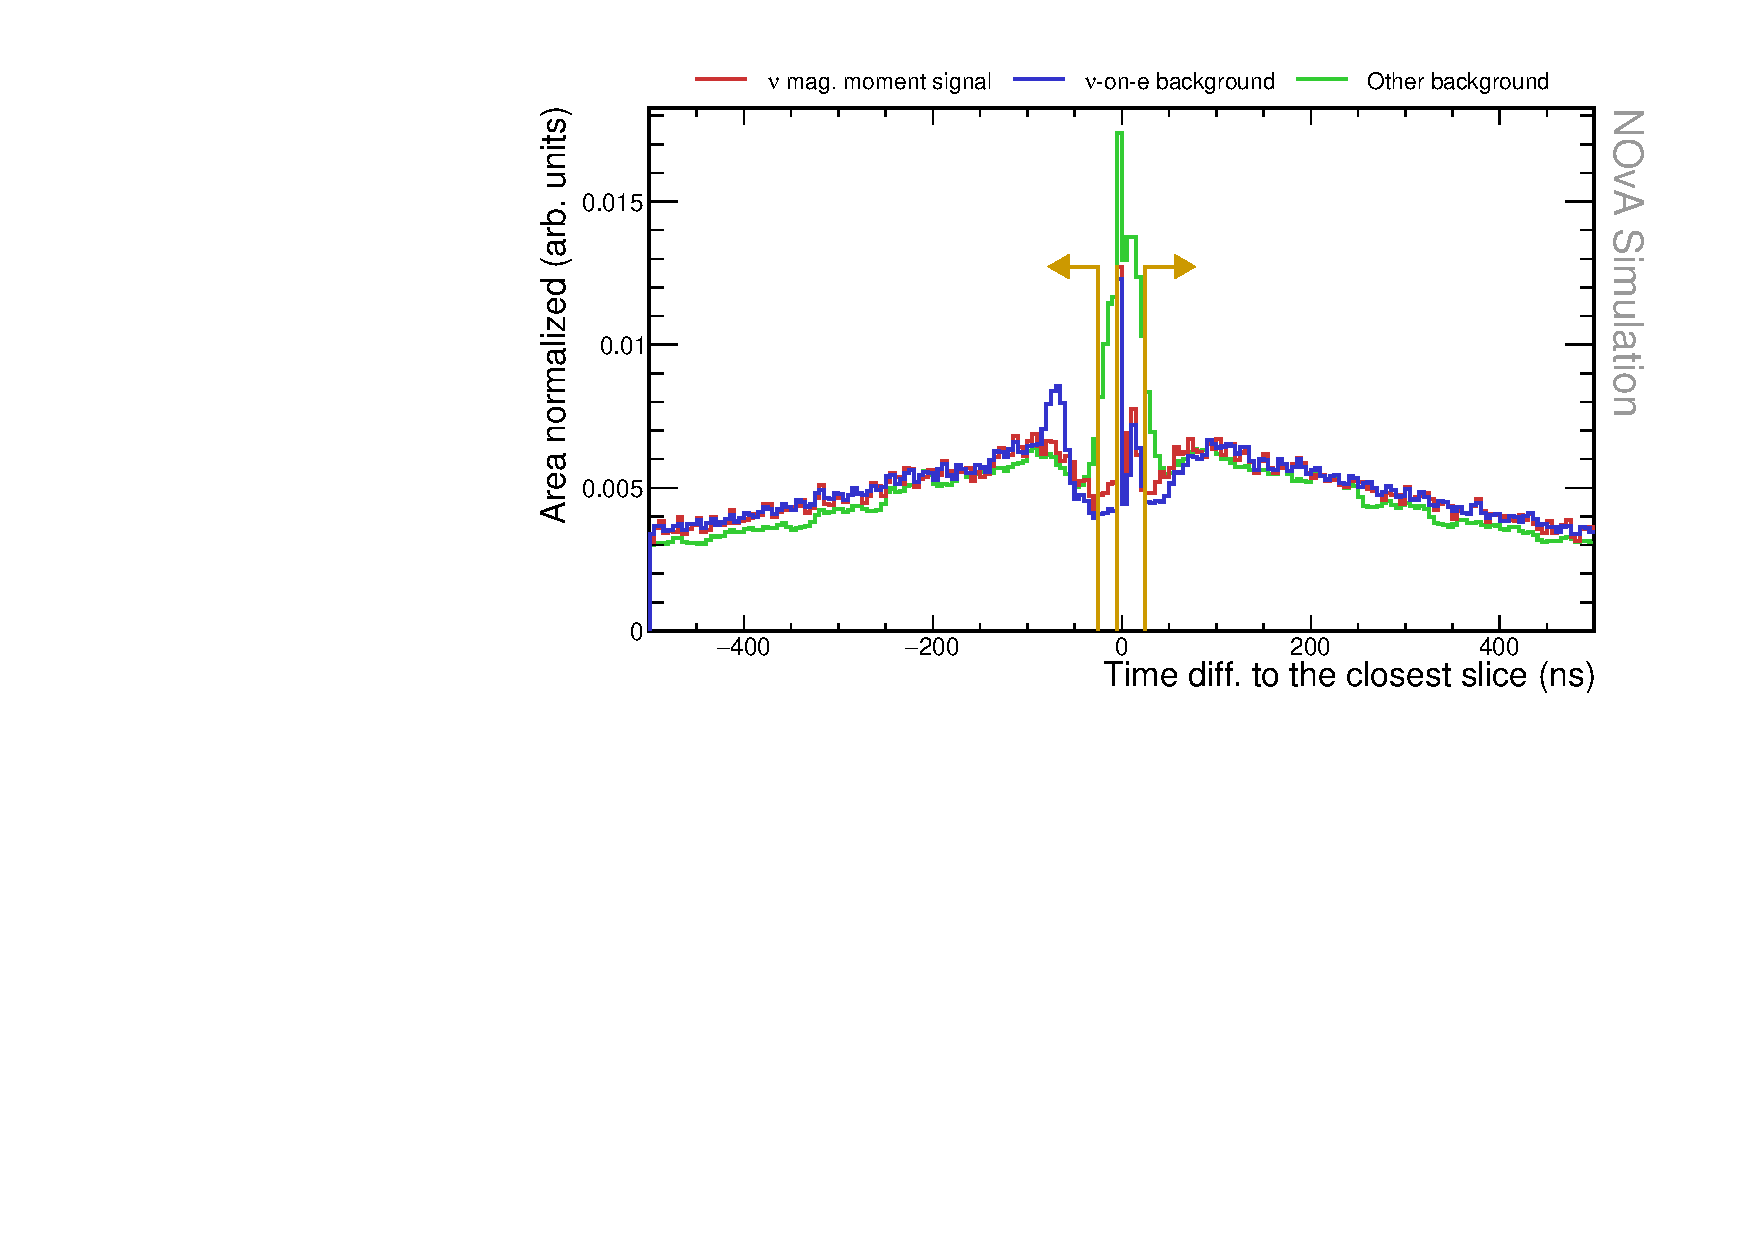
\includegraphics[width=.9\textwidth]{Plots/NuMMEventSelection/N1Cut_closestSlice.pdf}
\caption{Relative comparison of signal, $\nu$-on-e background, and other background events for pre-selection variables. Cuts on VtxIsValid and number of prongs were applied to make these plots. Gold lines show the cut values for the shown variables.}
\label{fig:PreSelectionCuts2}
\end{figure}

%\todo{Add the DeCAF cuts description here - might describe them already when introducing the decaf samples, not sure yet}

\subsubsection*{Fiducial and containment cuts}

\todo{Describe what does the fiducial cut do}
We require that the reconstructed vertex is contained within the following volume: $-185<\textsf{Vtx}_X<175,-175<\textsf{Vtx}_Y<175, 95<\textsf{Vtx}_Z<1095\ \unit{cm}$.

\begin{figure}[hbtp]
\centering
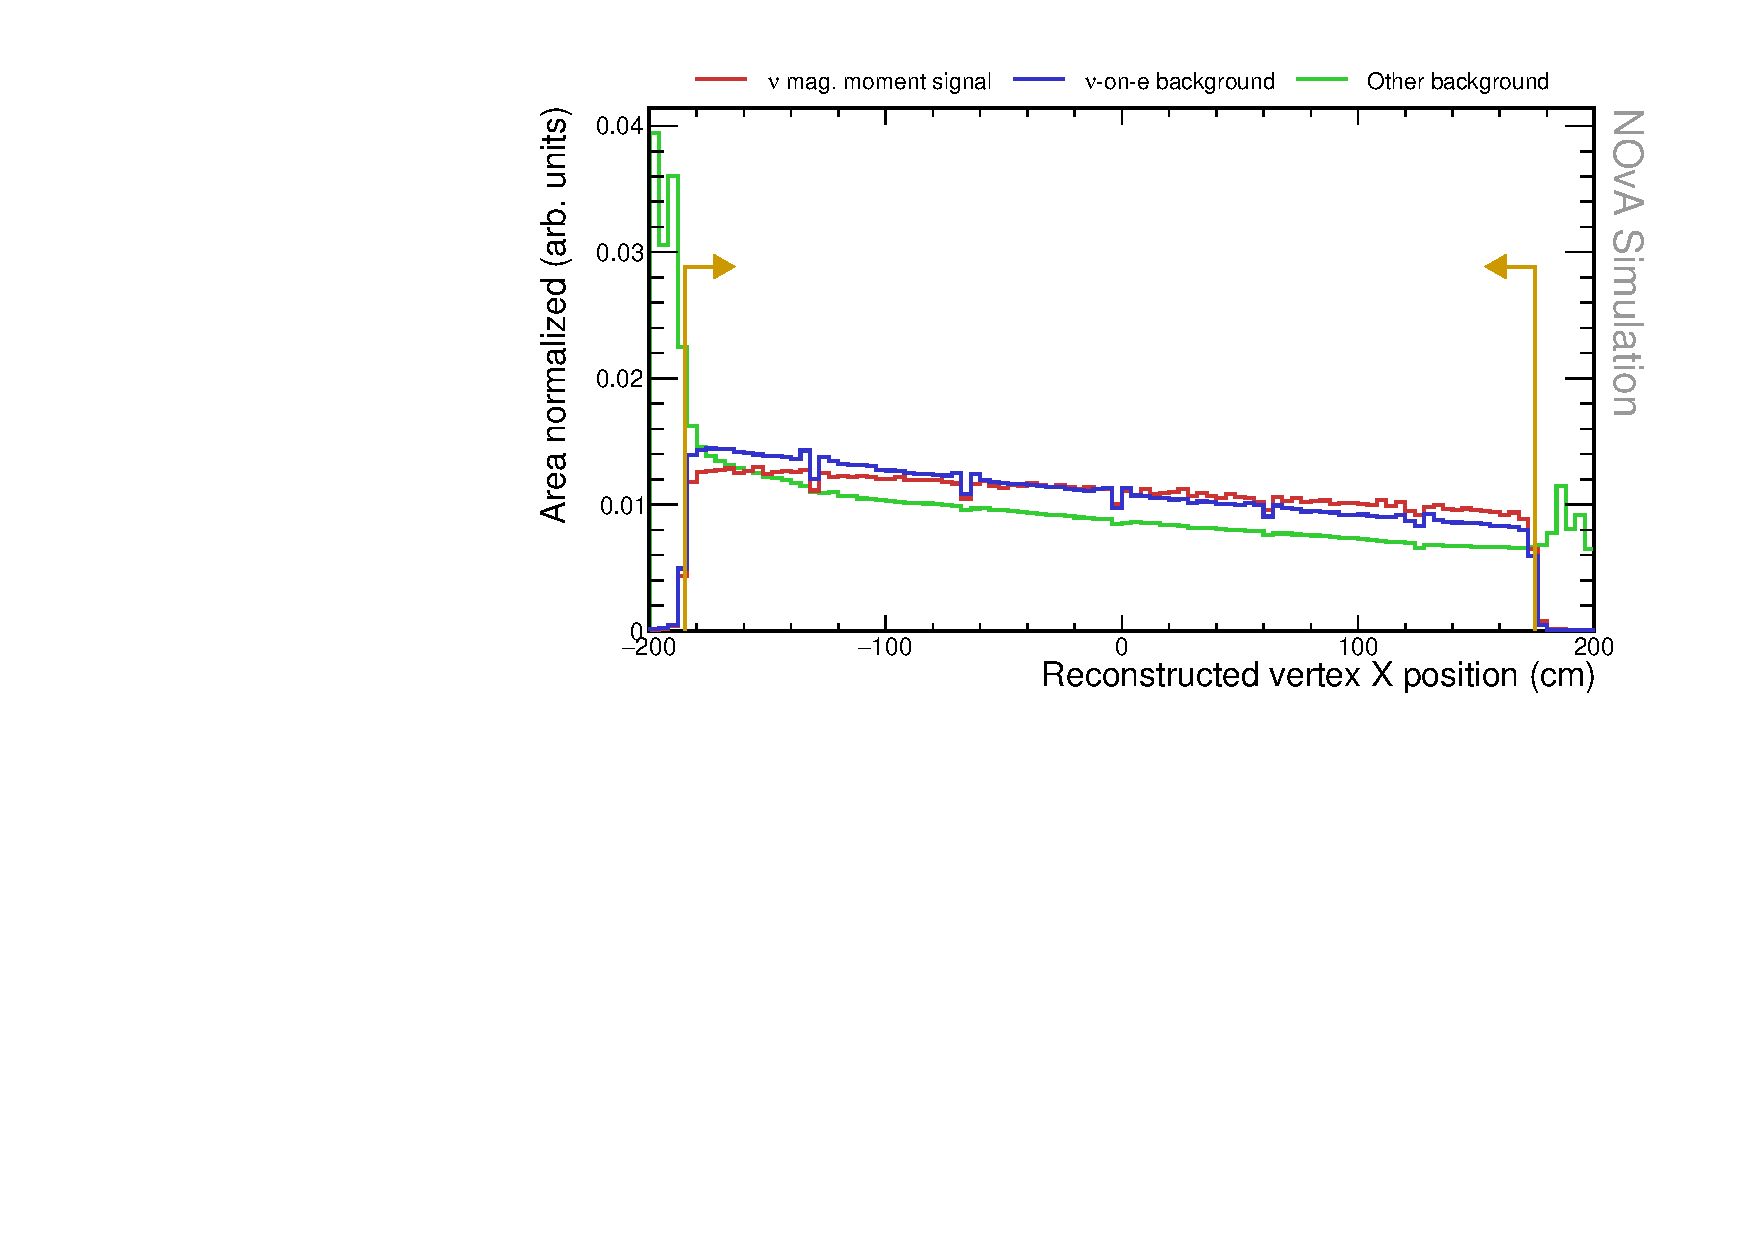
\includegraphics[width=.9\textwidth]{Plots/NuMMEventSelection/NoCut_vtxX.pdf}
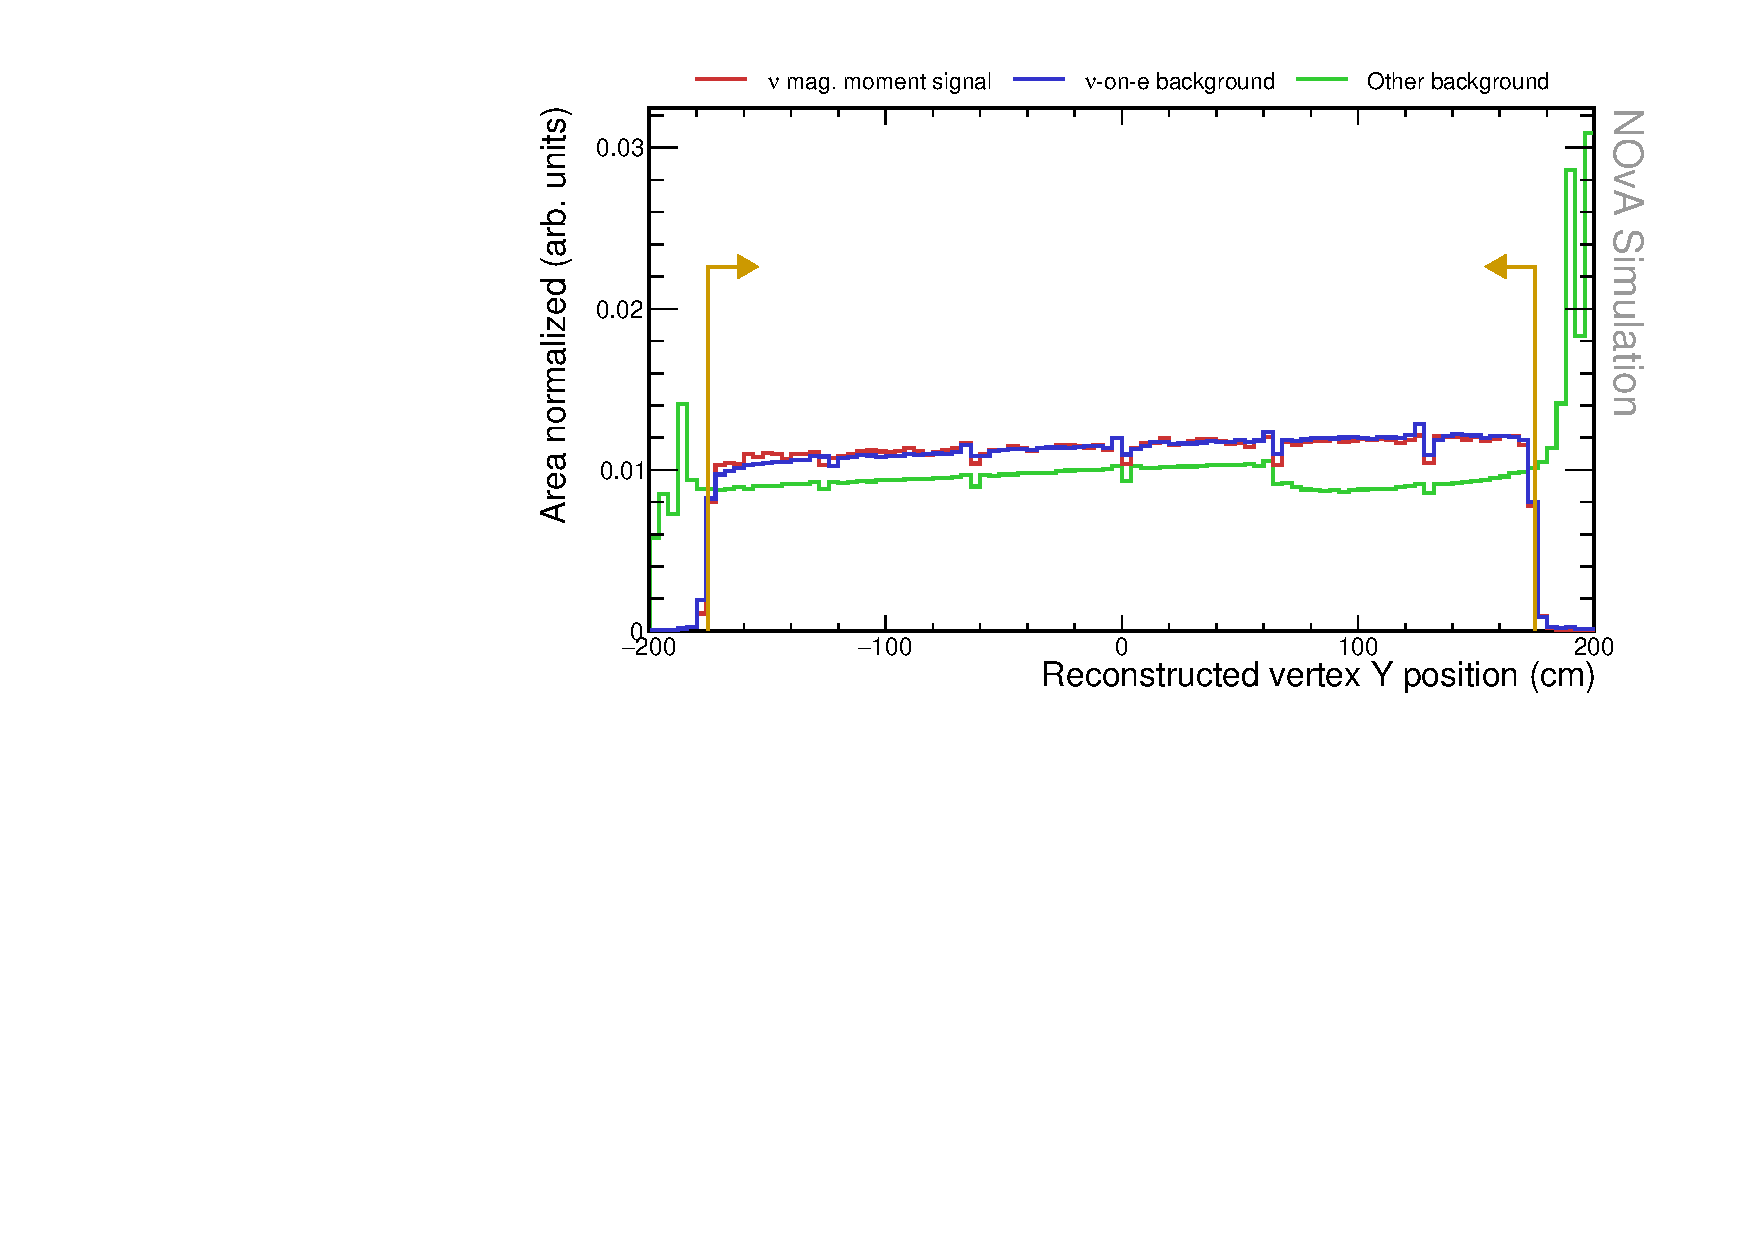
\includegraphics[width=.9\textwidth]{Plots/NuMMEventSelection/NoCut_vtxY.pdf}
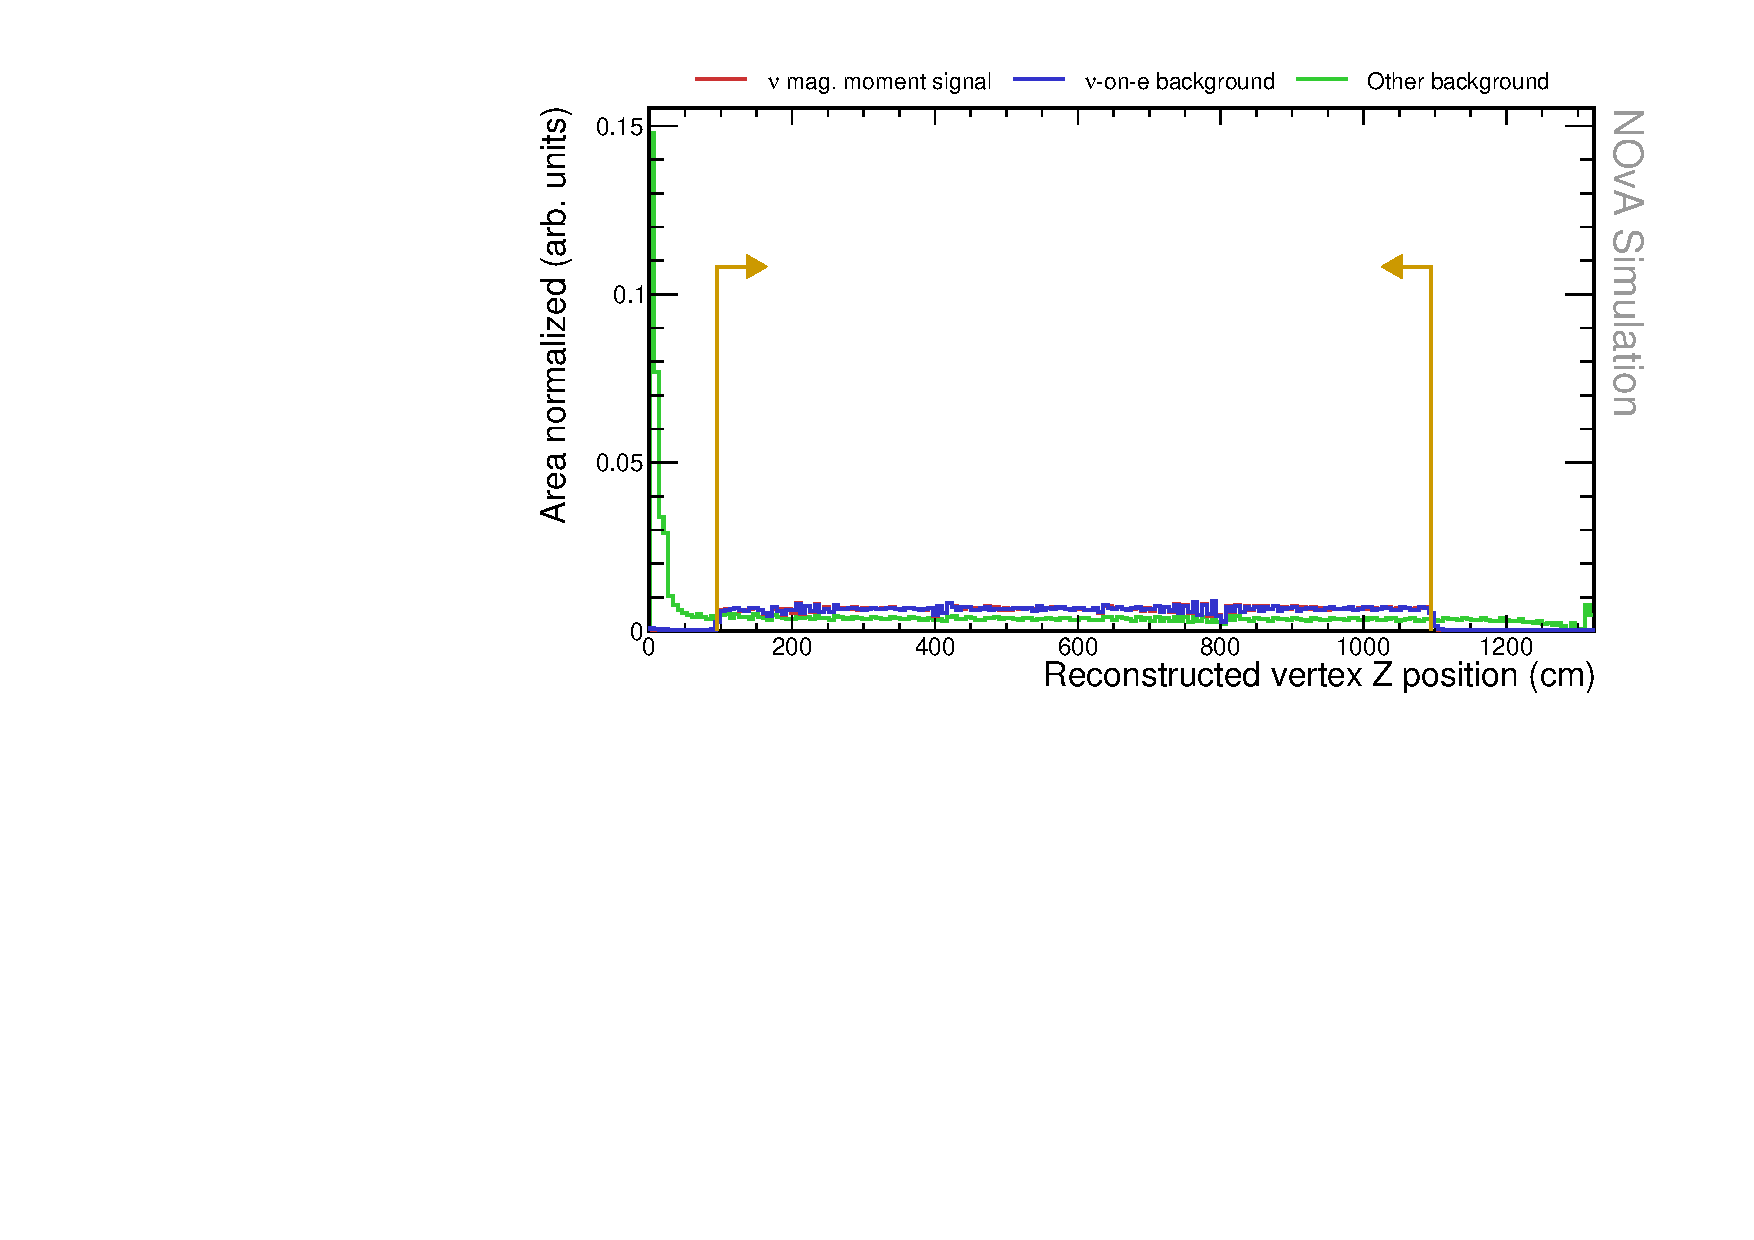
\includegraphics[width=.9\textwidth]{Plots/NuMMEventSelection/NoCut_vtxZ.pdf}
\caption{Relative comparison of signal, $\nu$-on-e background, and other background events for the reconstructed vertex. No cuts were applied to make these plots. Gold lines show the cut values that create the fiducial volume.}
\label{fig:FiducialCut}
\end{figure}

To ensure all the energy is contained within the detector and to remove events originating outside of the detector (rock muons), we require that the extreme positions of hits for all prongs in the slice are within the following volume: $-190<\textsf{min}_X, \textsf{max}_X<180, -180<\textsf{min}_Y, \textsf{max}_Y<190, 105<\textsf{min}_Z, \textsf{max}_Z<1275\ \unit{cm}$.

\begin{figure}[hbtp]
\centering
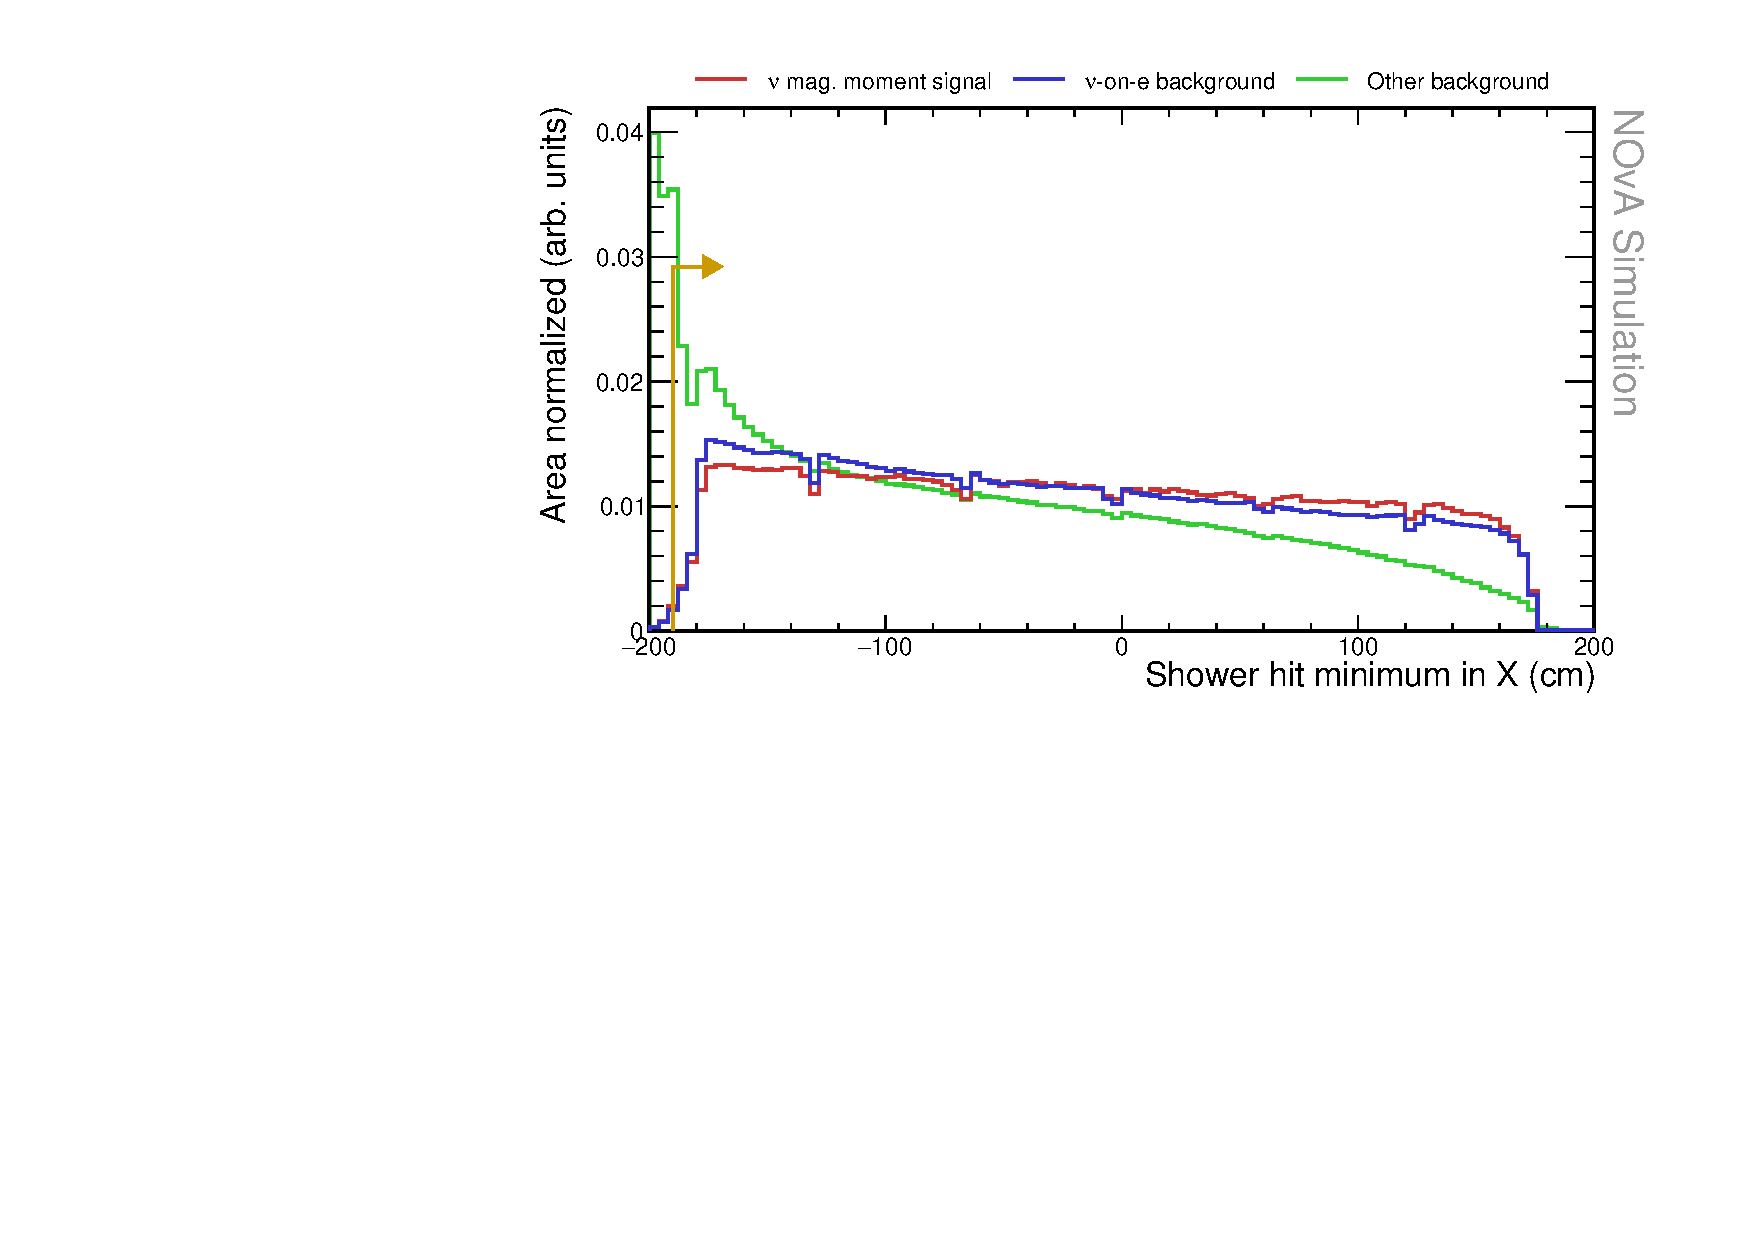
\includegraphics[width=.9\textwidth]{Plots/NuMMEventSelection/N1Cut_minX.pdf}
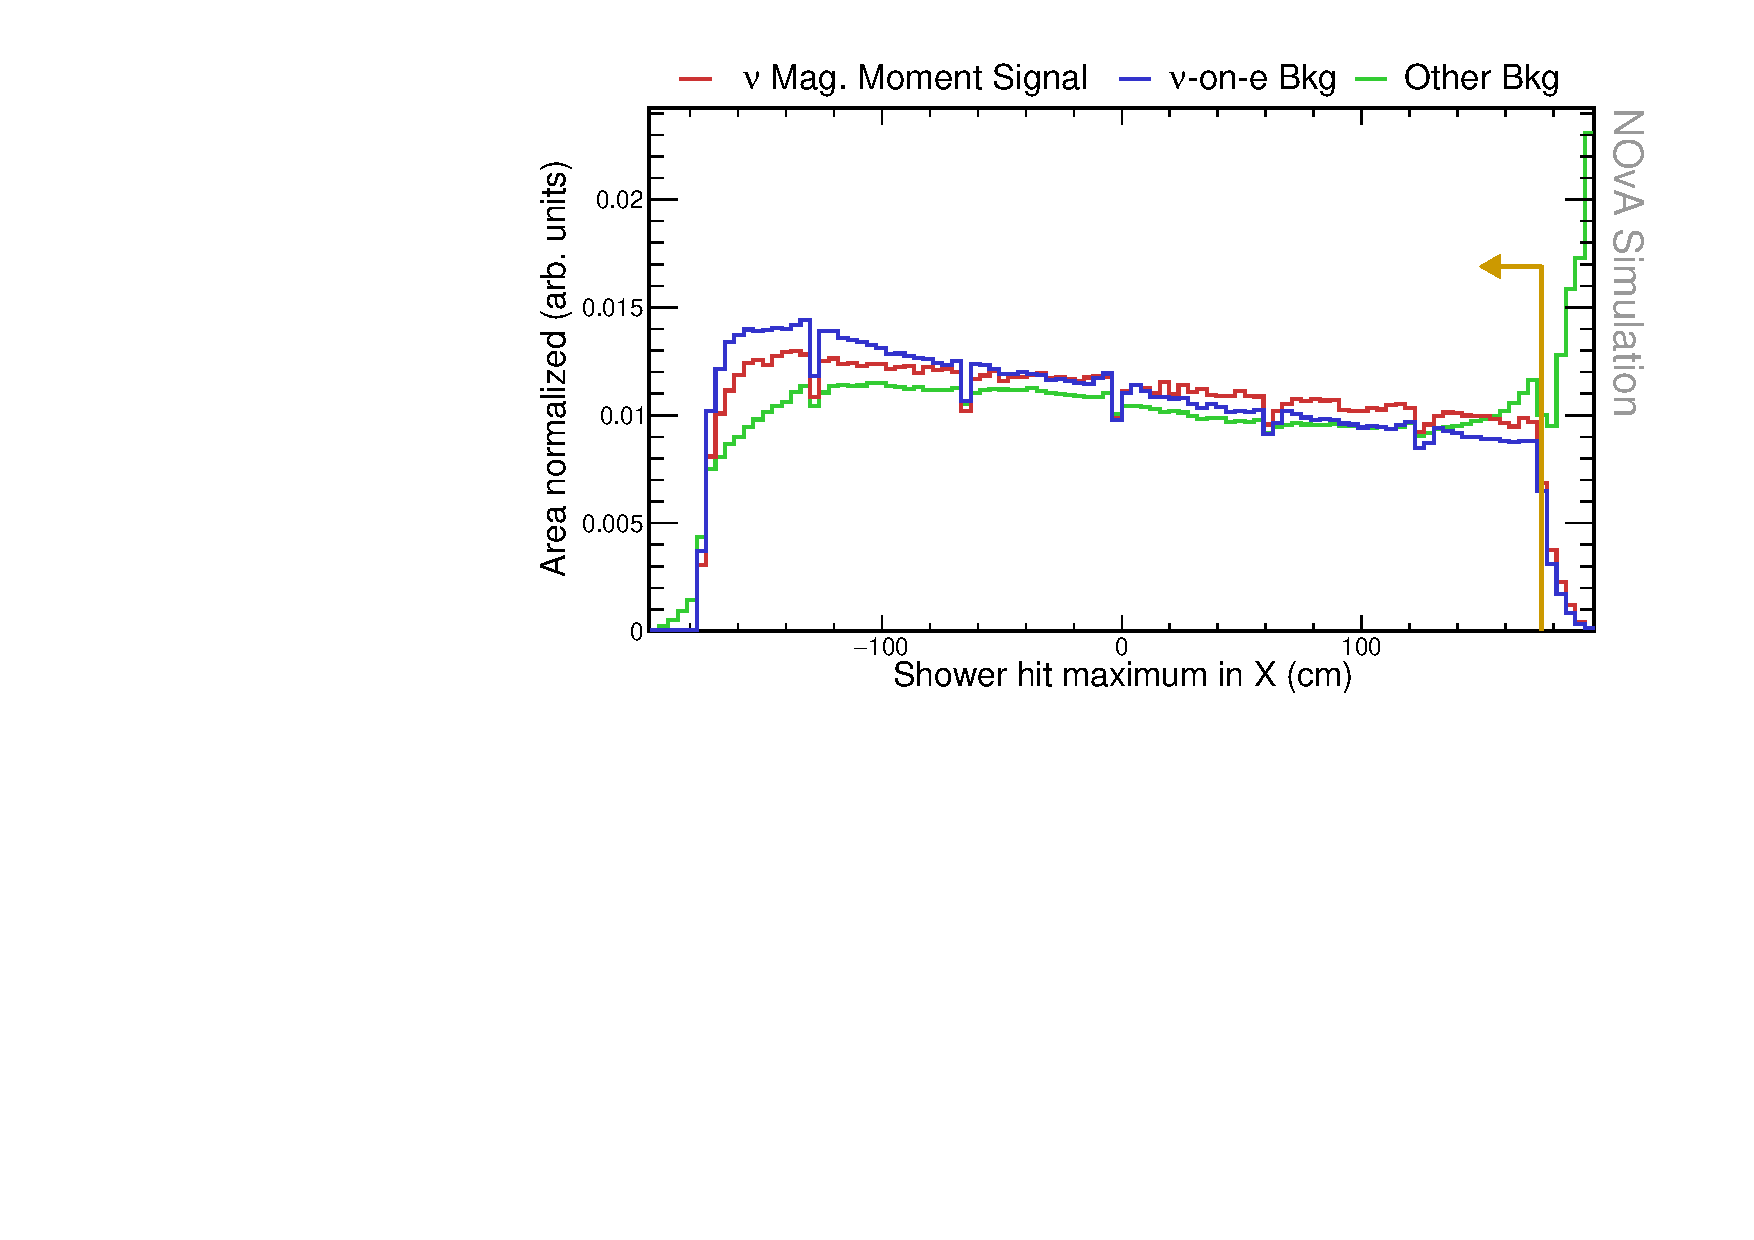
\includegraphics[width=.9\textwidth]{Plots/NuMMEventSelection/N1Cut_maxX.pdf}
\caption{Relative comparison of signal, $\nu$-on-e background, and other background events for the minimum and maximum position of the reconstructed shower along the x axis. Pre-selection and fiducial cuts were applied to make these plots. Gold lines show the values of the containment cuts.}
\label{fig:ContainmentCutsX}
\end{figure}

\begin{figure}[hbtp]
\centering
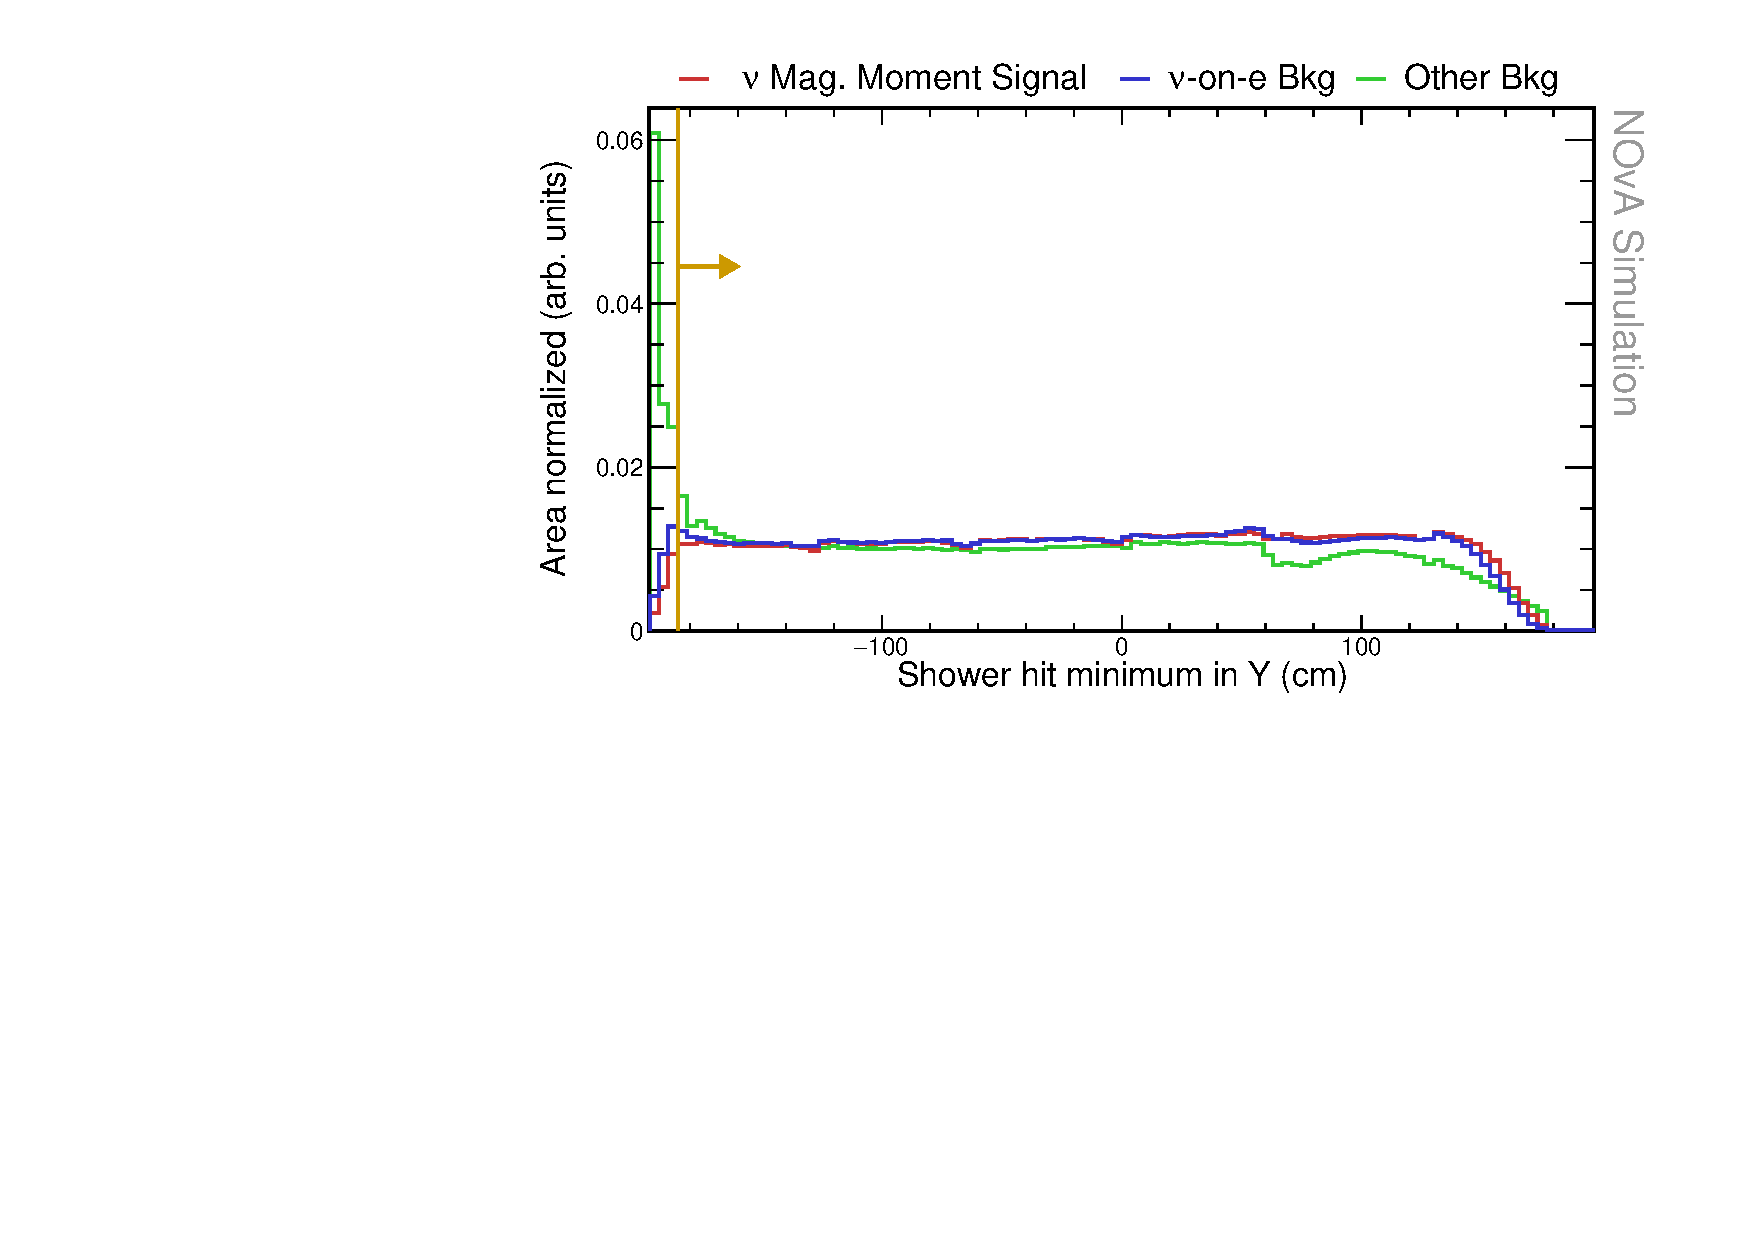
\includegraphics[width=.9\textwidth]{Plots/NuMMEventSelection/N1Cut_minY.pdf}
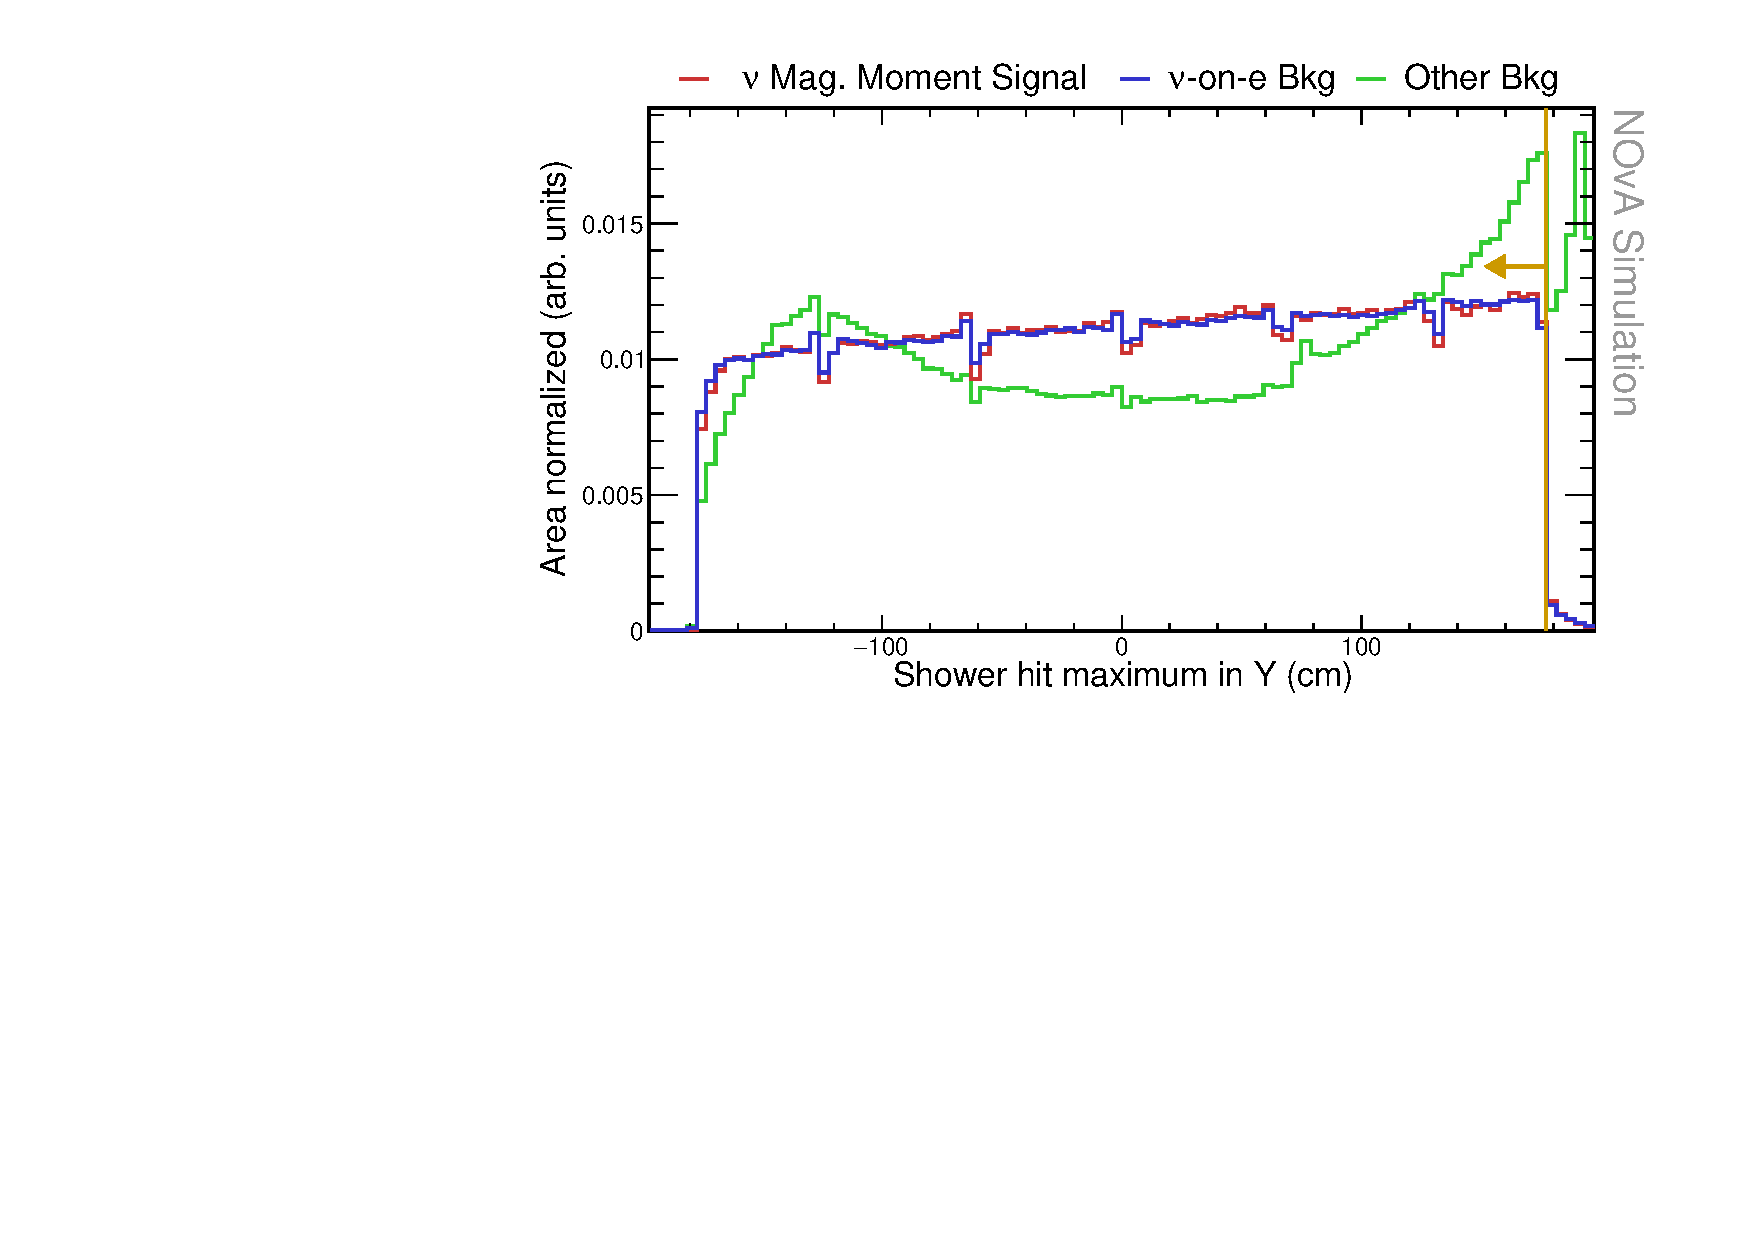
\includegraphics[width=.9\textwidth]{Plots/NuMMEventSelection/N1Cut_maxY.pdf}
\caption{Relative comparison of signal, $\nu$-on-e background, and other background events for the minimum and maximum position of the reconstructed shower along the Y axis. Pre-selection and fiducial cuts were applied to make these plots. Gold lines show the values of the containment cuts.}
\label{fig:ContainmentCutsY}
\end{figure}

\begin{figure}[hbtp]
\centering
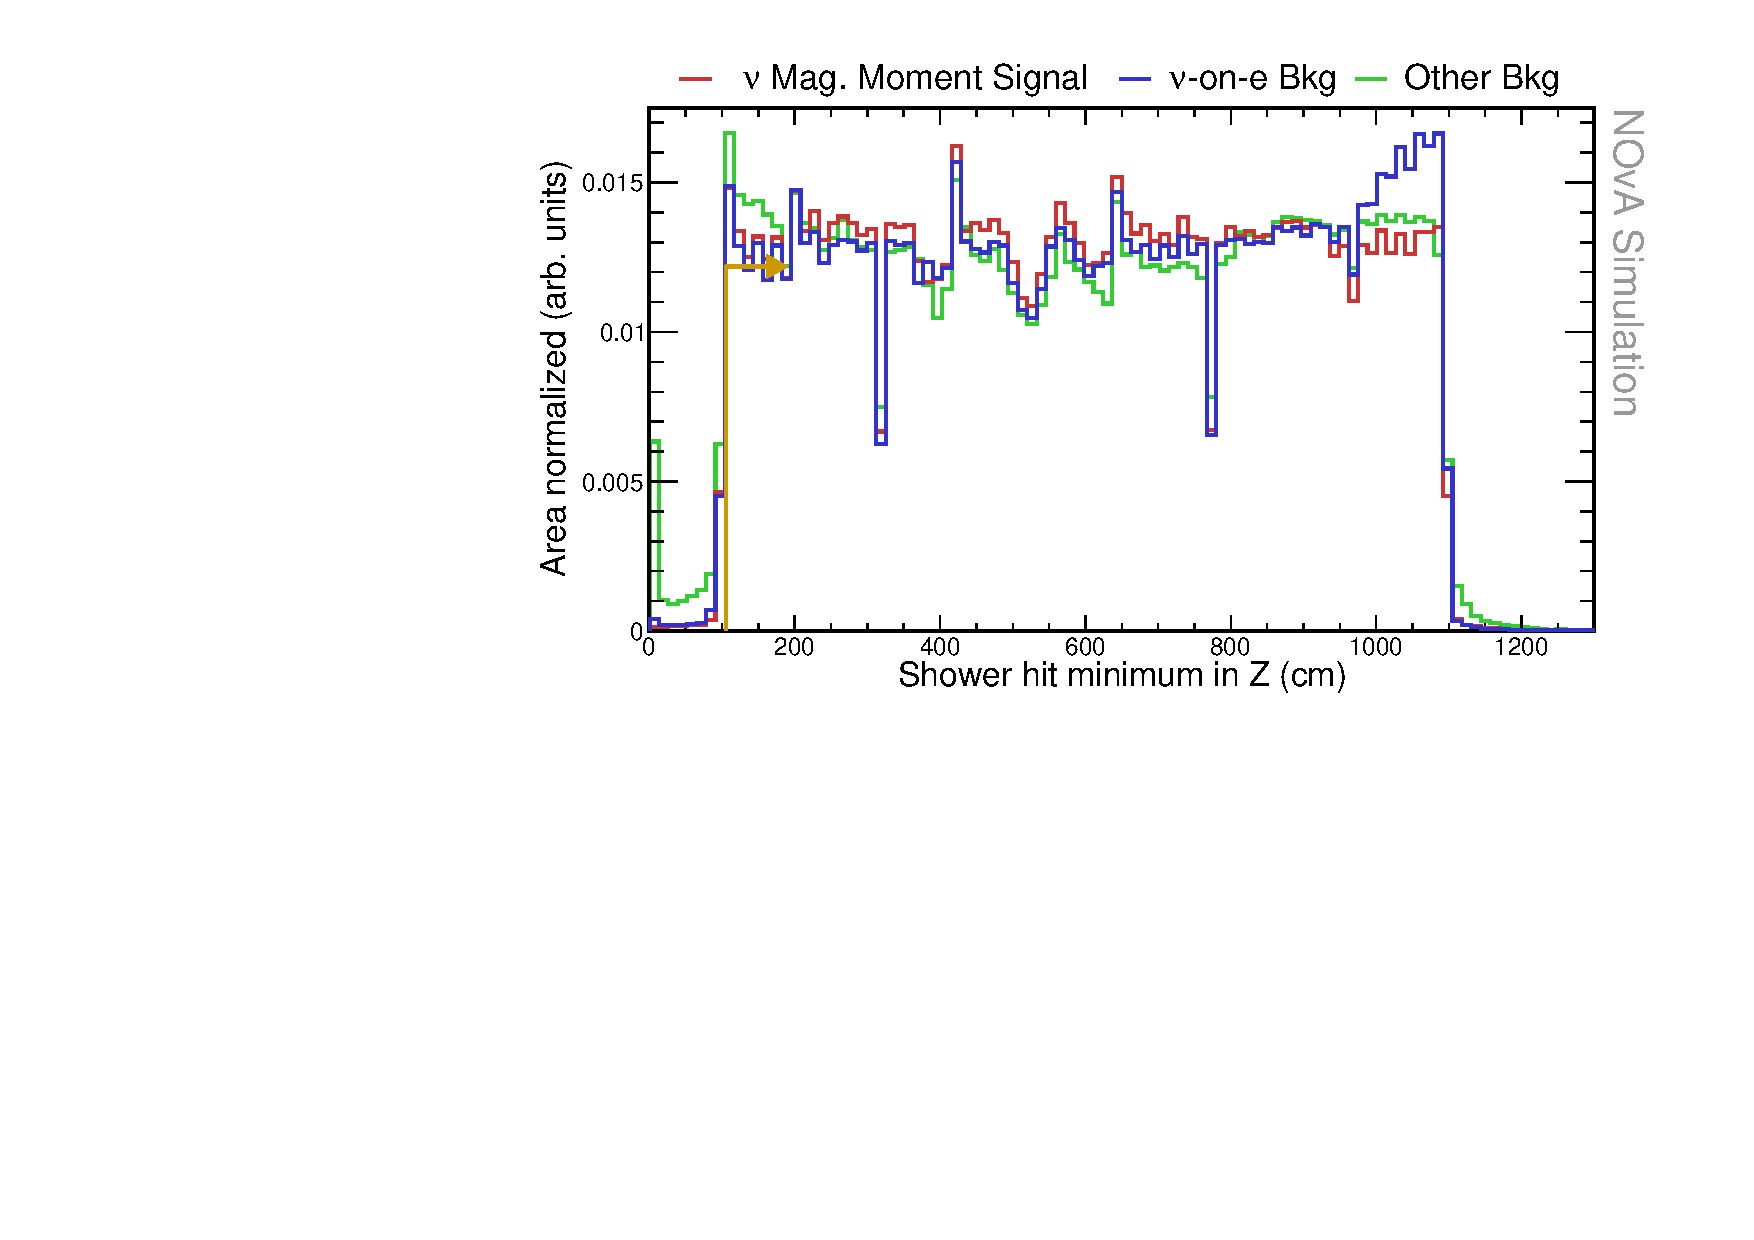
\includegraphics[width=.9\textwidth]{Plots/NuMMEventSelection/N1Cut_minZ.pdf}
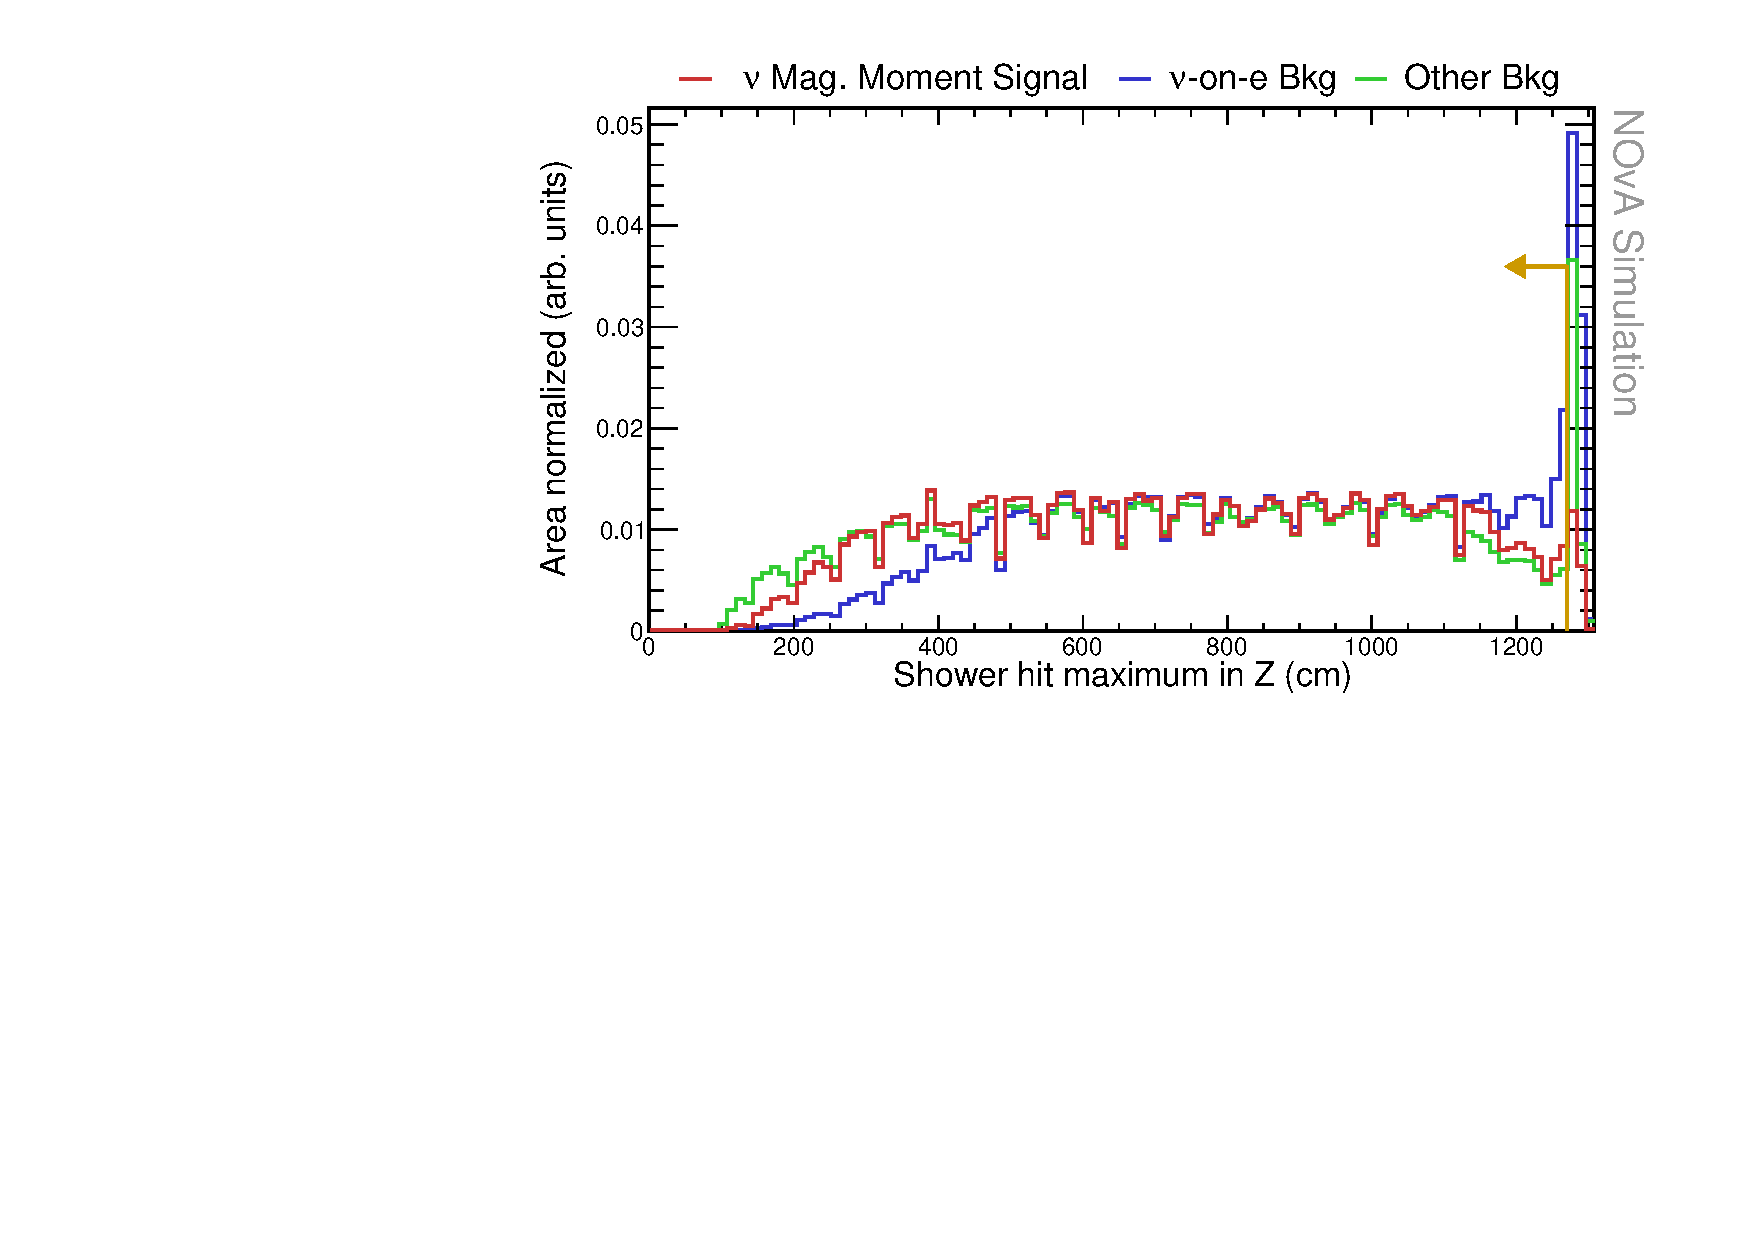
\includegraphics[width=.9\textwidth]{Plots/NuMMEventSelection/N1Cut_maxZ.pdf}
\caption{Relative comparison of signal, $\nu$-on-e background, and other background events for the minimum and maximum position of the reconstructed shower along the Z axis. Pre-selection and fiducial cuts were applied to make these plots. Gold lines show the values of the containment cuts.}
\label{fig:ContainmentCutsZ}
\end{figure}

\subsubsection*{Single particle requirement}

To selection events with a single particle we require that the fraction of energy contained in the most energetic shower is $>0.8$, that the summed energy of all cells (above threshold and within $\pm8$ planes from the vertex) outside of the most energetic shower is $<0.02\ \unit{GeV}$, and that the distance between the vertex and the start of the primary shower is $<20\ \unit{cm}$.

\begin{figure}[hbtp]
\centering
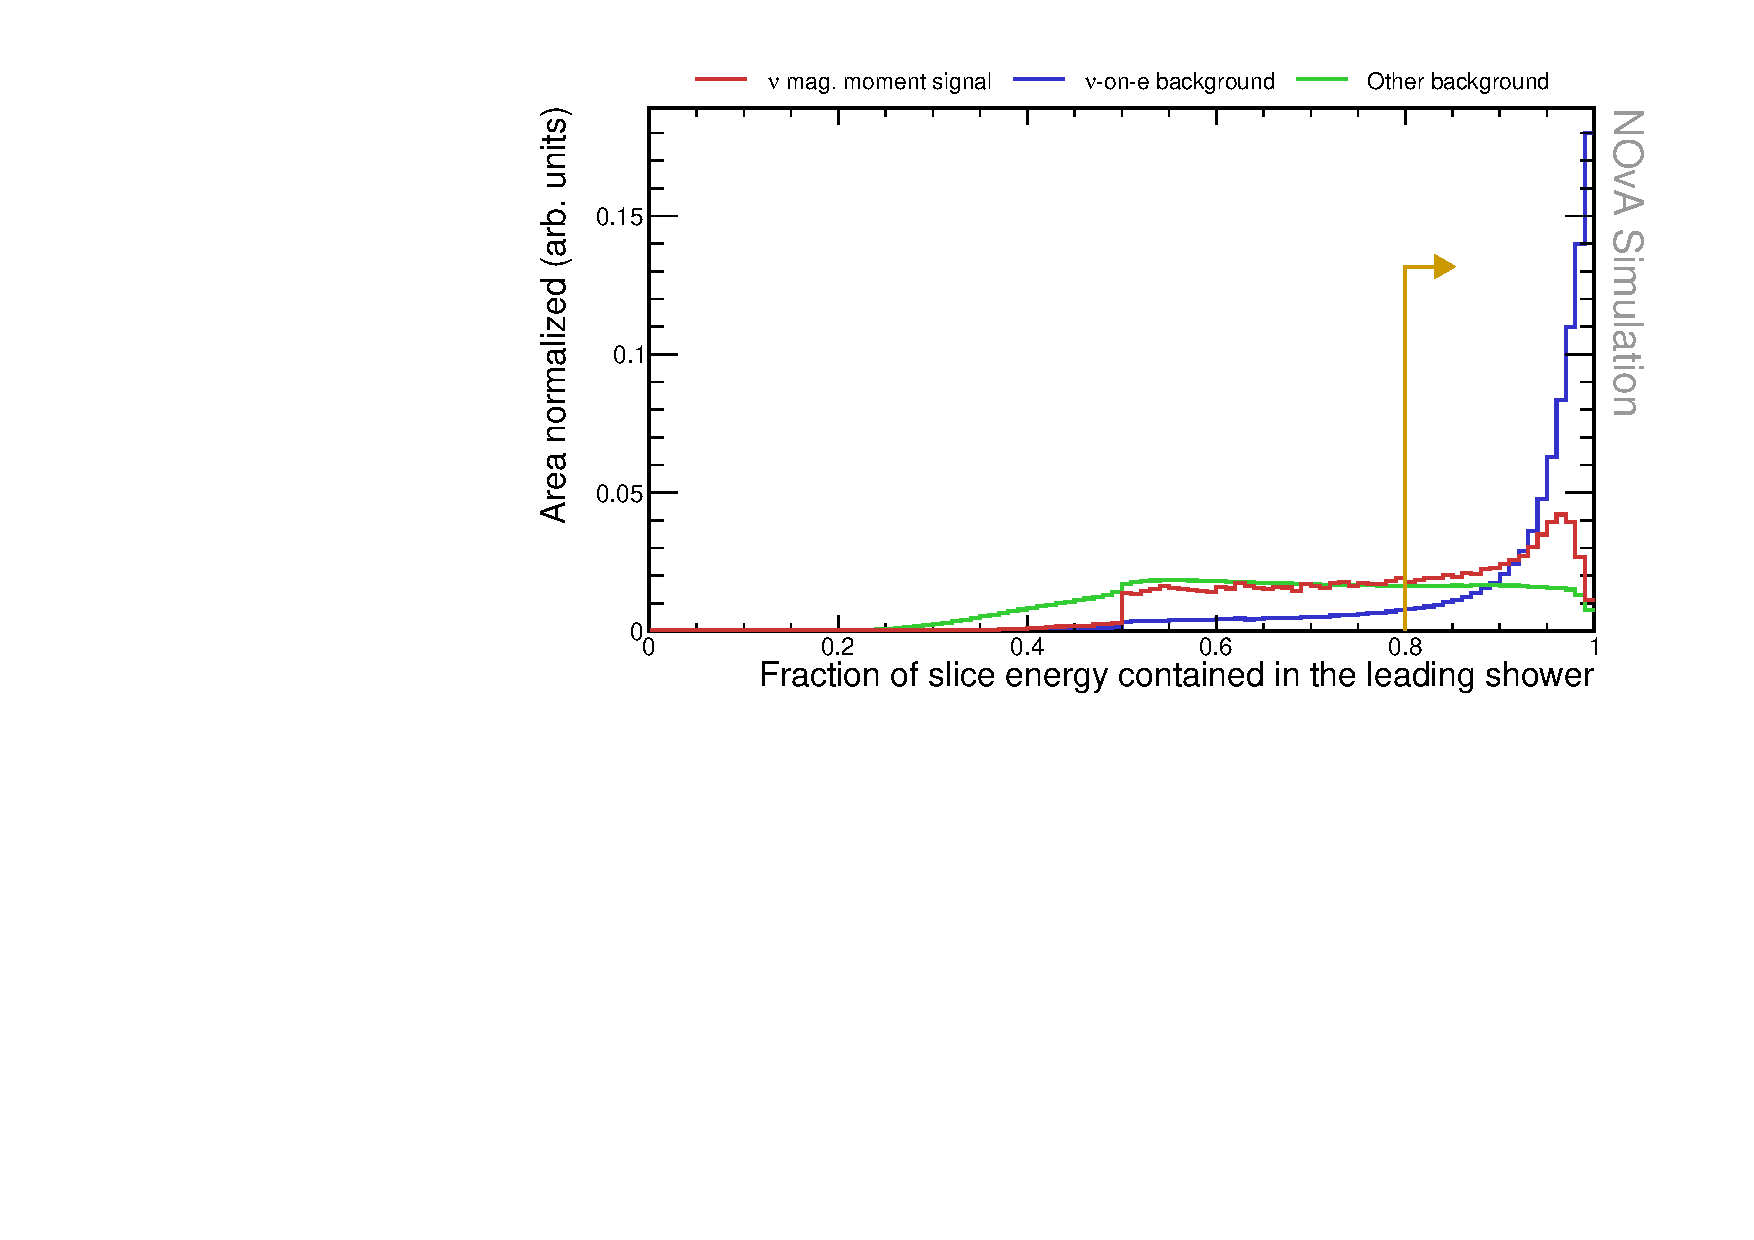
\includegraphics[width=.9\textwidth]{Plots/NuMMEventSelection/N1Cut_showerEFrac.pdf}
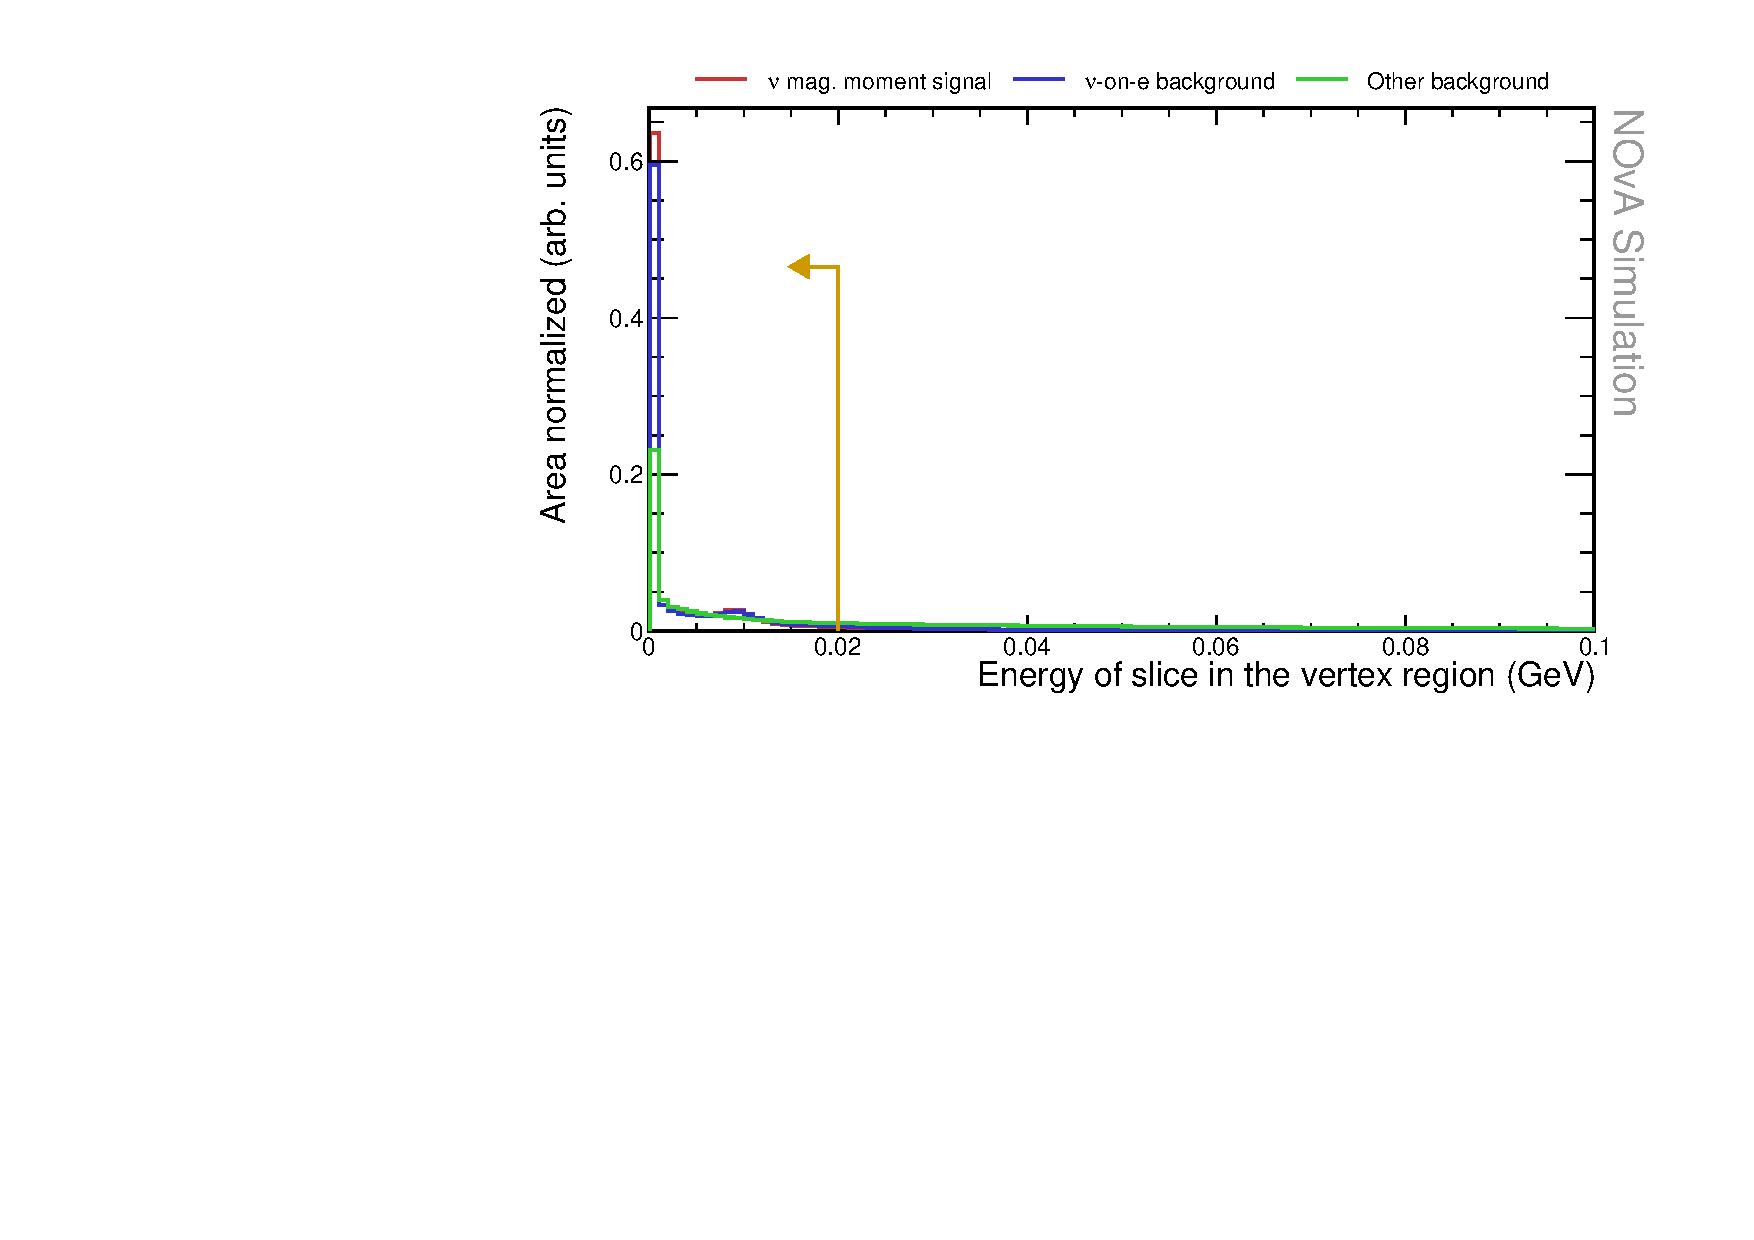
\includegraphics[width=.9\textwidth]{Plots/NuMMEventSelection/N1Cut_vtxE.pdf}
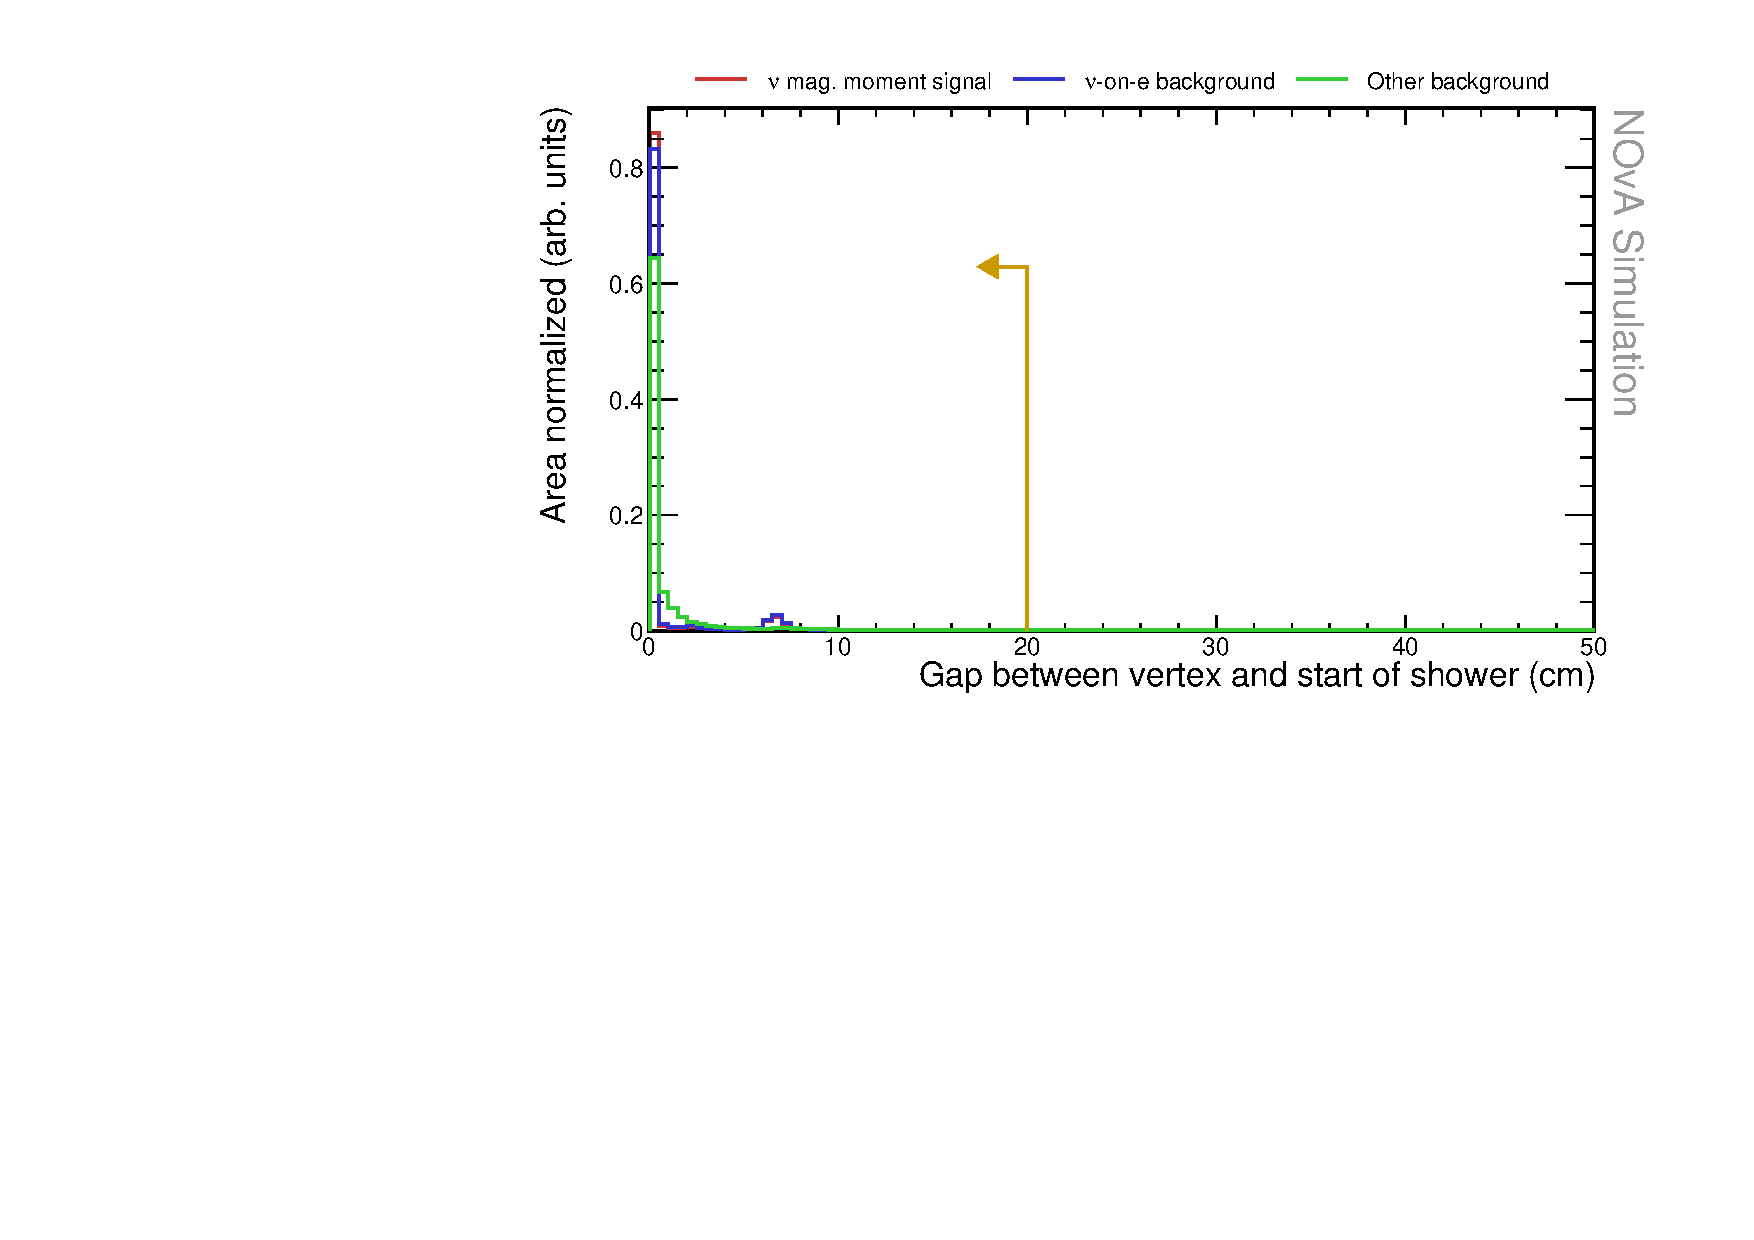
\includegraphics[width=.9\textwidth]{Plots/NuMMEventSelection/N1Cut_gap.pdf}
\caption{Relative comparison of signal, $\nu$-on-e background, and other background events for the reconstructed vertex. No cuts were applied to make these plots. Gold lines show the cut values that create the fiducial volume.}
\label{fig:SingleShowerCuts}
\end{figure}

\subsubsection*{Shower energy cut}

\todo{discuss the energy cut, should this be removed? What is the effect on the event count? Why was this included in the first place (the identifiers are not as strong for lower energies - is this true though? - also there are further unexplored backgrounds that would need to be further studied and explore. Maybe depends on where would we move the cut...)}
The calorimetric energy of the primary shower is required to be within $0.5<E_{cal}<5\ \unit{GeV}$.

\begin{figure}[hbtp]
\centering
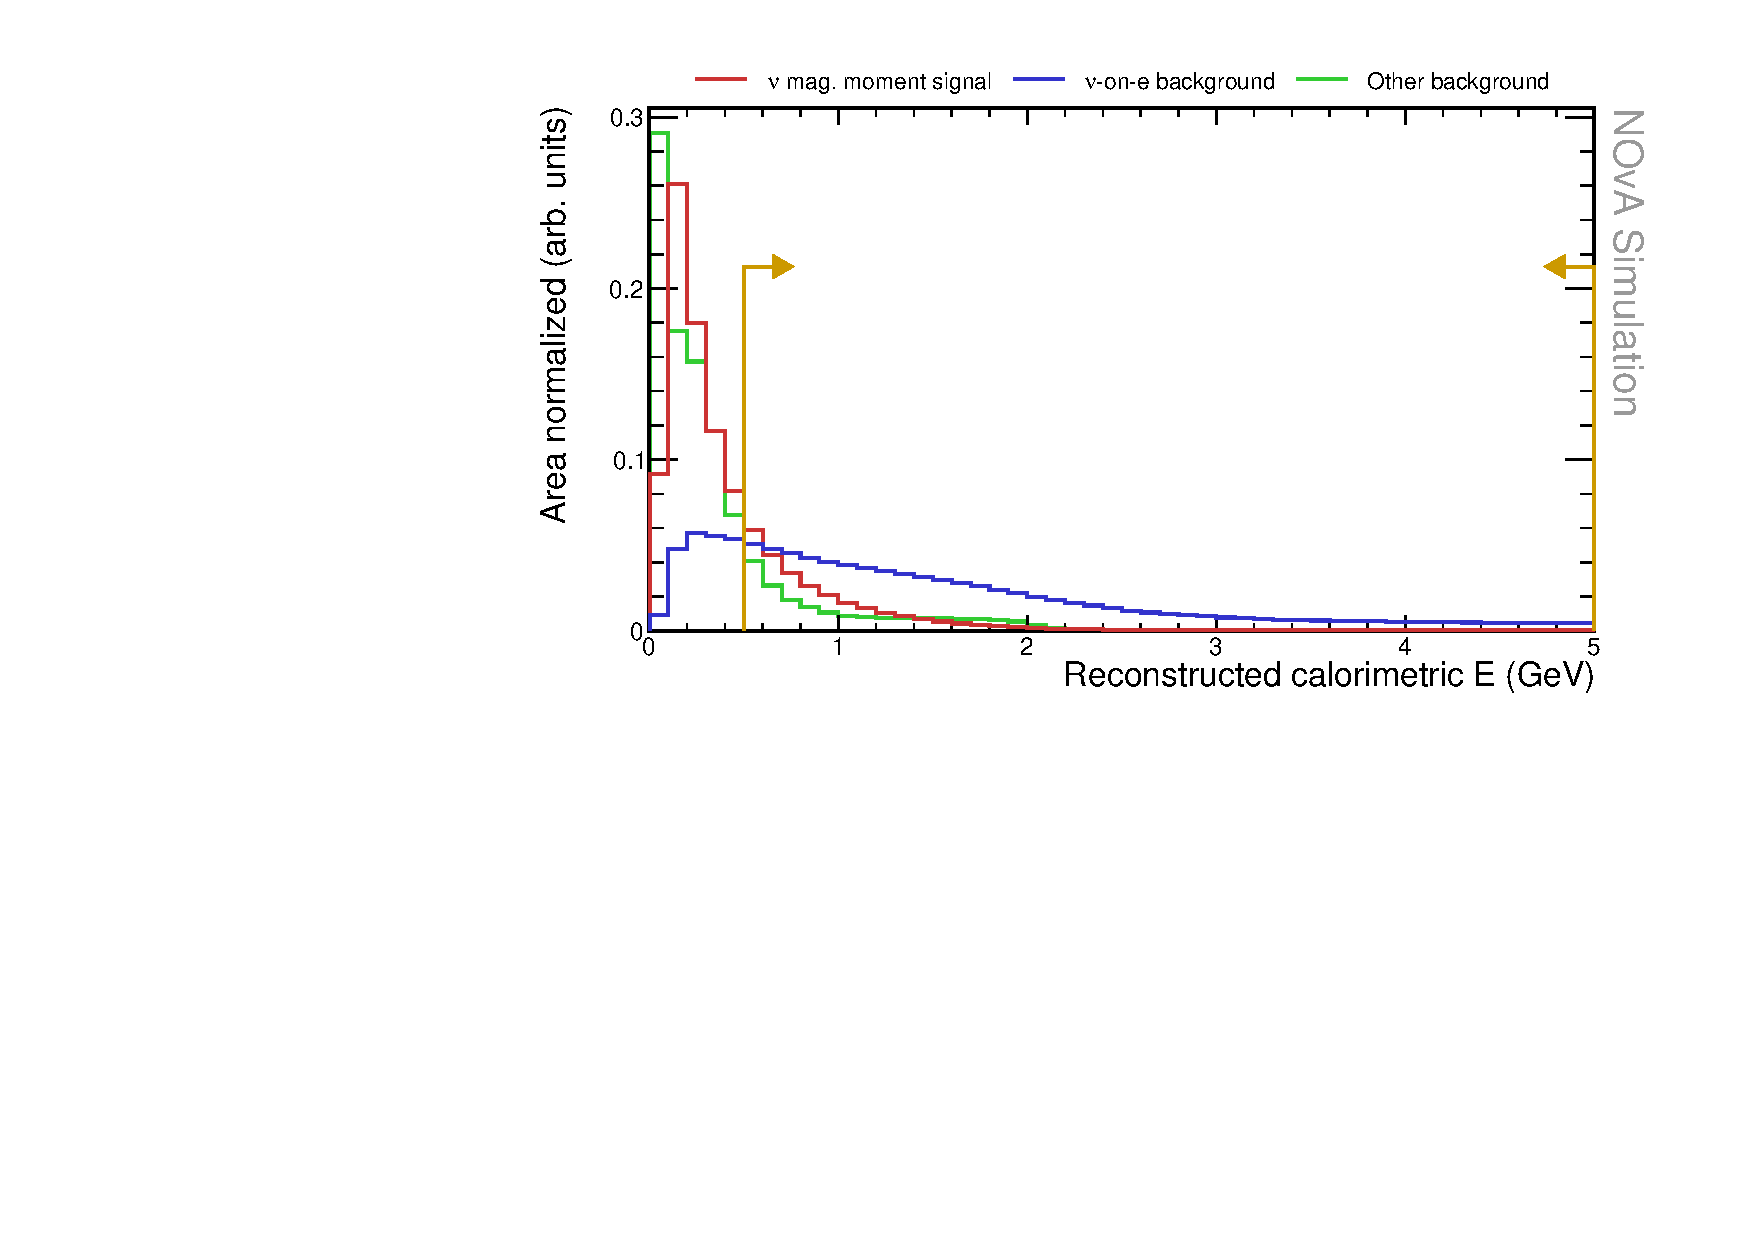
\includegraphics[width=.9\textwidth]{Plots/NuMMEventSelection/N1Cut_calE.pdf}
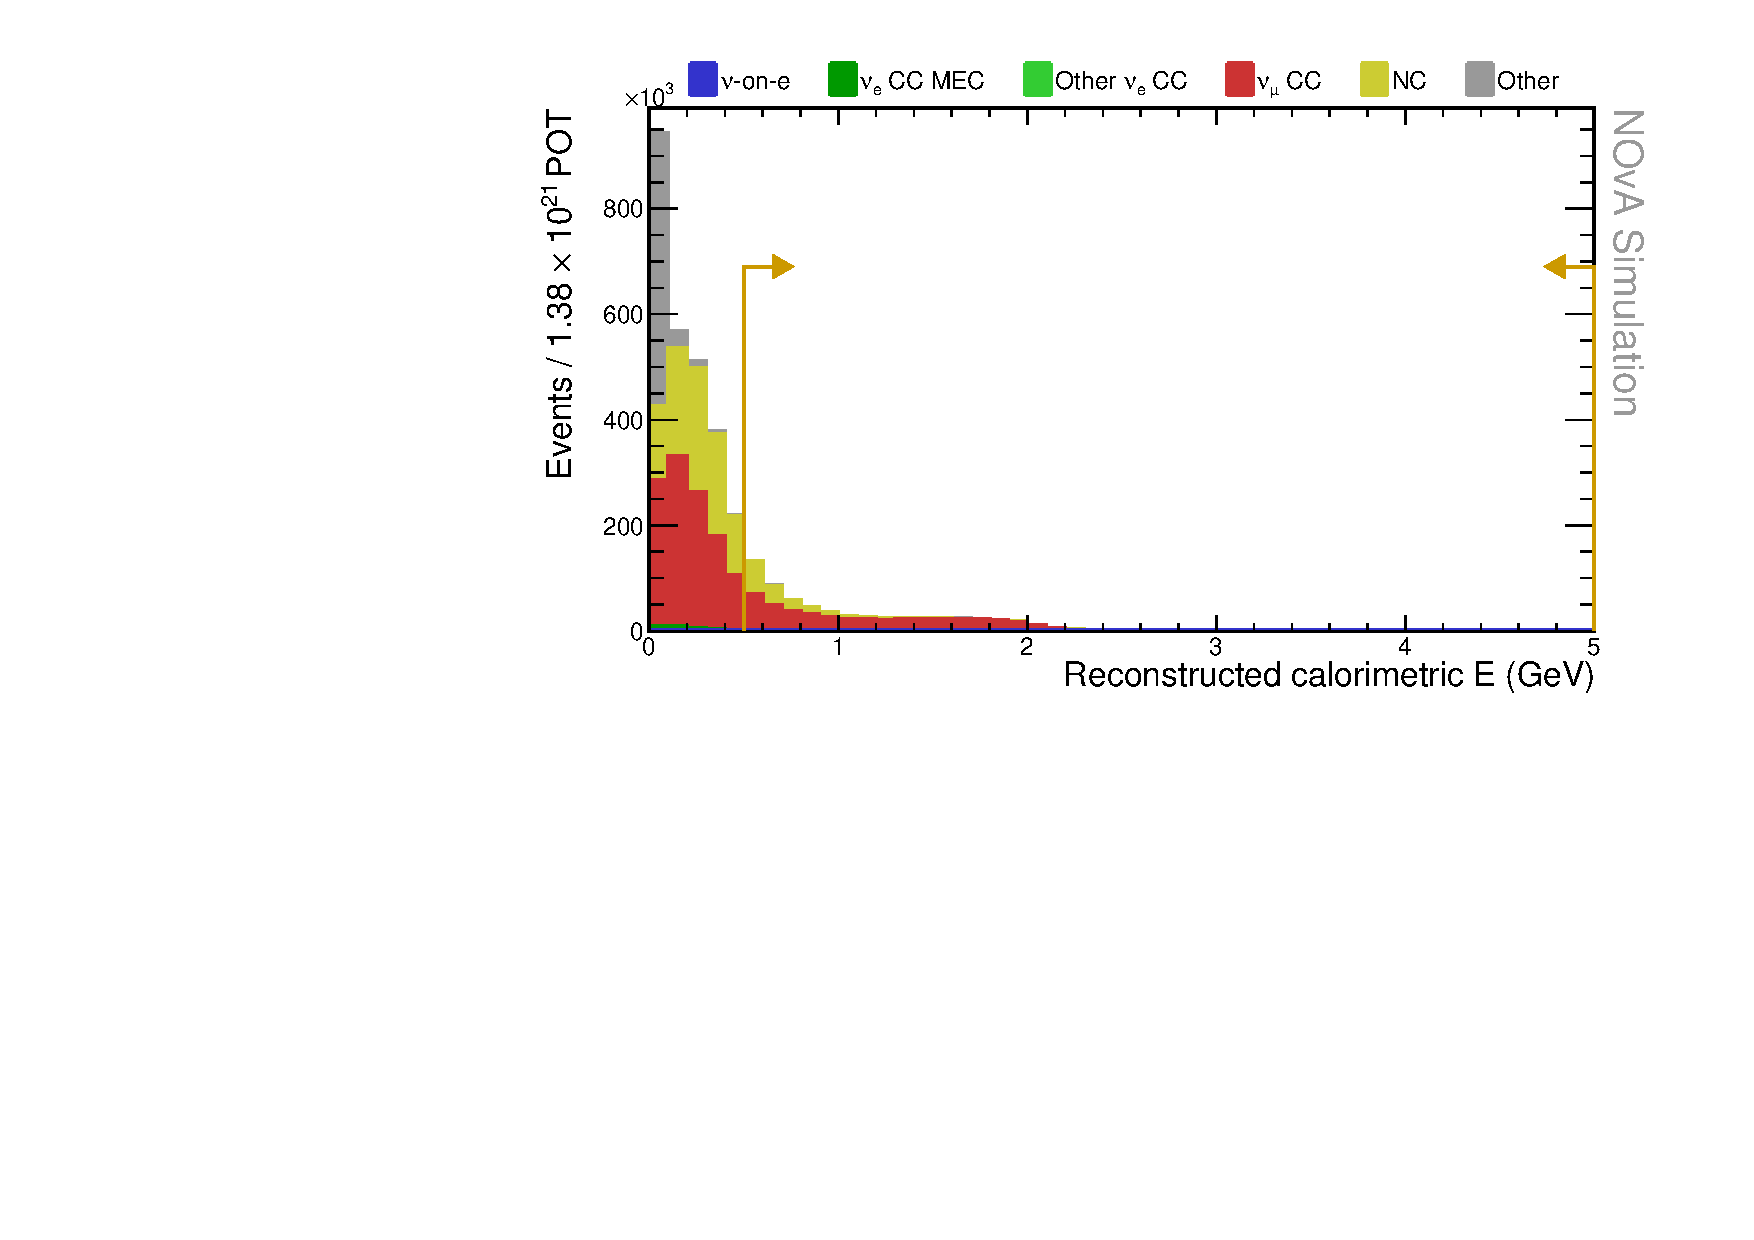
\includegraphics[width=.9\textwidth]{Plots/NuMMEventSelection/N1Cut_calE_BkgDecomp.pdf}
\caption{Relative comparison of signal, $\nu$-on-e background, and other background events for the reconstructed vertex. No cuts were applied to make these plots. Gold lines show the cut values that create the fiducial volume.}
\label{fig:SingleShowerCuts1}
\end{figure}

\begin{figure}[hbtp]
\centering
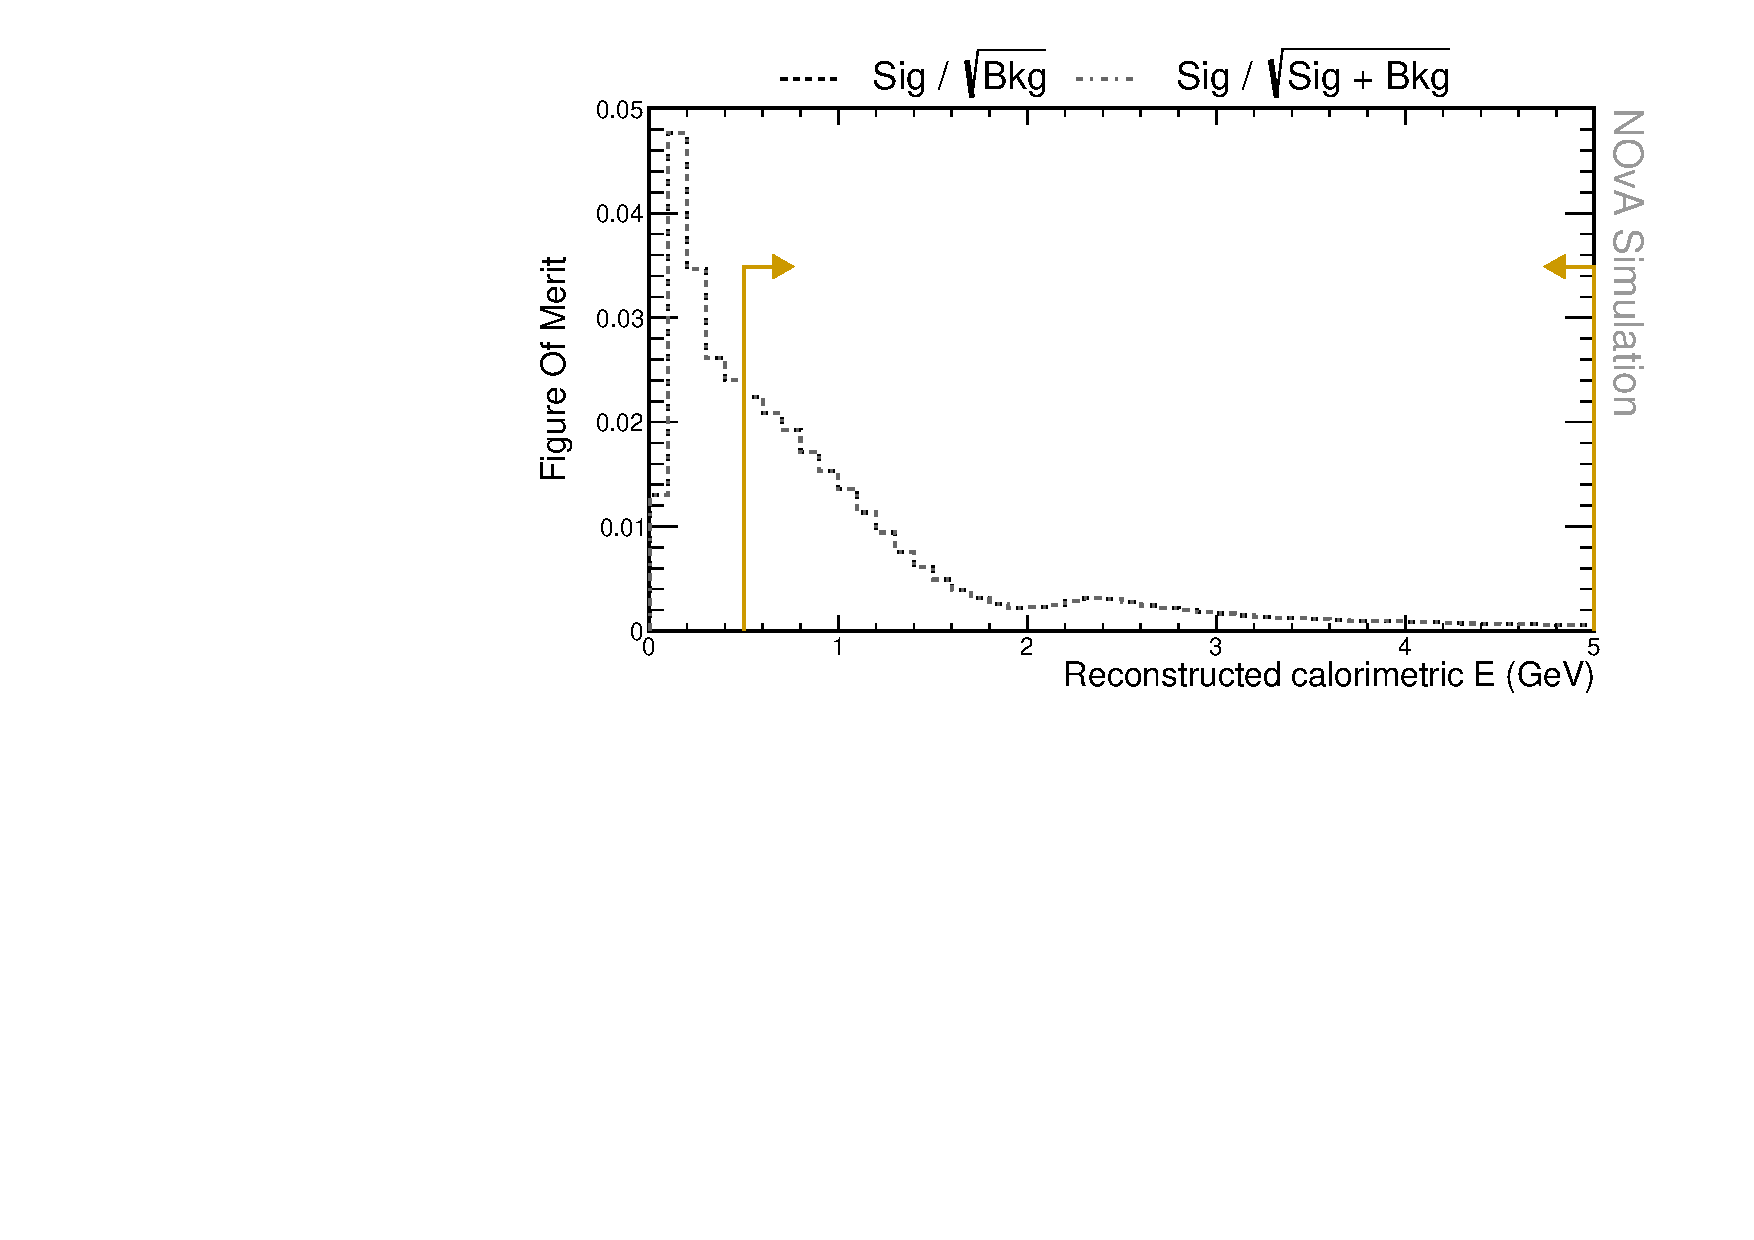
\includegraphics[width=.9\textwidth]{Plots/NuMMEventSelection/NuMM_N1Cut_calE_Stat.pdf}
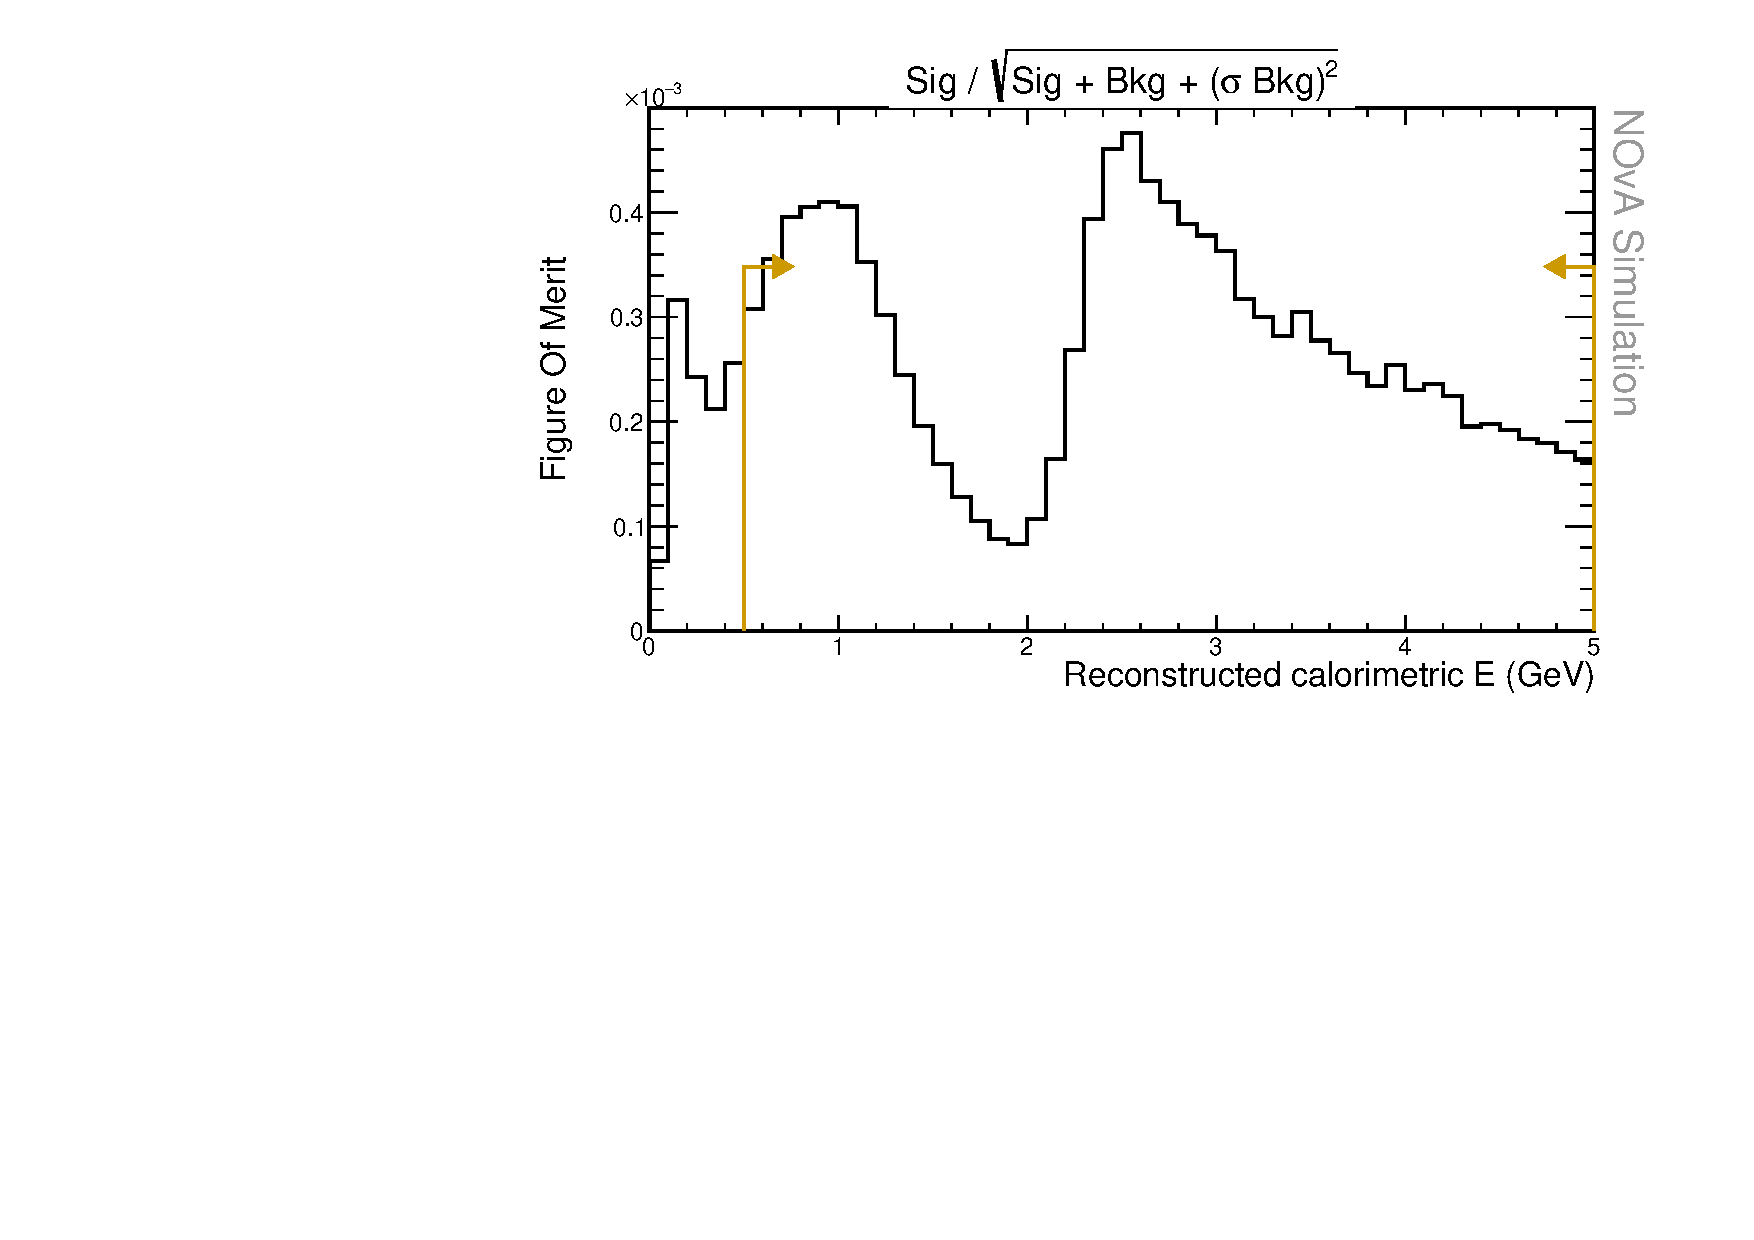
\includegraphics[width=.9\textwidth]{Plots/NuMMEventSelection/NuMM_N1Cut_calE_Syst.pdf}
\caption{Relative comparison of signal, $\nu$-on-e background, and other background events for the reconstructed vertex. No cuts were applied to make these plots. Gold lines show the cut values that create the fiducial volume.}
\label{fig:SingleShowerCuts2}
\end{figure}

\subsubsection*{Event classifiers}

We are using two event classifiers based on convolution neural network that were developed specifically to identify $\nu$-on-e interactions. The first one (\texttt{NuoneID}) is trained to select $\nu$-on-e events and the second one (\texttt{Epi0ID}) is trained on the events passing the \texttt{NuoneID} to reject the $\pi^0$ background. Our selection requires that \texttt{NuoneID}$>0.73$ and that \texttt{Epi0ID}$>0.92$.

\todo{reference theory for the kinematics of nuone scattering}
We require that the product of reconstructed energy of the primary shower and the square of its angle from the Z axis is $E_{cal}\theta^2<0.005\ \unit{GeV\times rad^2}$.

\todo{Add plots of distributions of the event selection variables with two columns. LHS shows no cuts applied and RHS shows all previous cuts applied}

Using the many plots below that show the effect of each of the cuts on the signal and all background events. (For signal we are showing NuMM=...)

\todo{Describe the cutflow tables below}
The final event count and efficiency of each of the cuts is shown on the table \ref{tab:CutflowTableSignal}. Table \ref{tab:CutflowTableBackground} shows the dissemination of background into the individual components.

\begin{table}[!hb]
\caption{Event selection cutflow table}
\begin{tabular}{|l|ccc|ccc|ccc|}\hline
\multicolumn{1}{|c|}{}                                     & \multicolumn{3}{c|}{\textbf{$\nu$ Mag. Moment signal}}          & \multicolumn{3}{c|}{\textbf{$\nu$-on-e background}}                      & \multicolumn{3}{c|}{\textbf{Other background}}                           \\
\multicolumn{1}{|c|}{\multirow{-2}{*}{\textbf{Selection}}} & \multicolumn{1}{c}{\textbf{$N_{sig}$}} & \textbf{$\epsilon^{N-1}$} & \textbf{$\epsilon \left(\%\right)$} & \multicolumn{1}{c}{\textbf{$N_{IBkg}$}} & \textbf{$\epsilon^{N-1}$} & \textbf{$\epsilon \left(\%\right)$} & \multicolumn{1}{c}{\textbf{$N_{Bkg}$}} & \textbf{$\epsilon^{N-1}$} & \textbf{$\epsilon \left(\%\right)$} \\\hline
\textbf{No Cut}      & 269.77            & 100 & 100 & 3.43$\times 10^3$           & 100 & 100                                     & 2.96$\times 10^8$          & 100                                                             & 100                                    \\
\textbf{Vtx Is Valid}  & 180.58            & 66.94                                                              & 66.94                                     & 3.33$\times 10^3$               & 96.94                                                               & 96.94                                      & 2.34$\times 10^8$          & 79.09                                                              & 79.09                                     \\
\textbf{N Prongs}        & 174.69            & 96.74                                                              & 64.76                                     & 3.23$\times 10^3$                             & 96.99                                                               & 94.02                                      & 8.66$\times 10^7$                     & 37.00                                                                 & 29.27                                     \\
\textbf{Png Length}  & 174.67            & 99.99                                                              & 64.75                                     & 3.22$\times 10^3$                                          & 99.64                                                               & 93.68                                      & 7.67$\times 10^7$                              & 88.56                                                              & 25.92                                     \\
\textbf{N Planes}      & 174.67            & 100                                                                & 64.75                                     & 3.22$\times 10^3$                                          & 99.98                                                               & 93.67                                      & 7.67$\times 10^7$          & 99.98                                                              & 25.92                                     \\
\textbf{N Cells}       & 174.67            & 100                                                                & 64.75                                     & 3.22$\times 10^3$                                           & 99.98                                                               & 93.65                                      & 7.42$\times 10^7$          & 96.78                                                              & 25.08                                     \\
\textbf{Closest Slc}  & 169.82            & 97.22                                                              & 62.95                                     & 3.14$\times 10^3$                                           & 97.54                                                               & 91.35                                      & 6.95$\times 10^7$          & 93.68                                                              & 23.49 \\
\textbf{Fiducial}     & 167.72            & 98.76                                                              & 62.17                                     & 3.09$\times 10^3$           & 98.41                                                               & 89.89                                      & 3.59$\times 10^7$          & 51.71                                                              & 12.15                                     \\
\textbf{Cont.}  & 159.37            & 95.02                                                              & 59.08                                     & 2.48$\times 10^3$           & 80.43                                                               & 72.30                                      & 1.38$\times 10^7$          & 38.35                                                              & 4.66                                      \\
\textbf{ShwE Frac.}  & 150.37            & 94.35                                                              & 55.74                                     & 2.42$\times 10^3$           & 97.59                                                               & 70.56                                      & 8.82$\times 10^6$          & 63.97                                                              & 2.98                                      \\
\textbf{Vtx E}         & 142.29            & 94.63                                                              & 52.74                                     & 2.18$\times 10^3$           & 90.16                                                               & 63.62                                      & 4.15$\times 10^6$          & 47.07                                                              & 1.40                                      \\
\textbf{Shw Gap}          & 137.96            & 96.96                                                              & 51.14                                     & 2.09$\times 10^3$           & 95.58                                                               & 60.80                                      & 3.25$\times 10^6$          & 78.34                                                              & 1.10                                      \\
\textbf{Shw E}      & 37.13             & 26.92                                                              & 13.76                                     & 1.36$\times 10^3$           & 65.10                                                               & 39.58                                      & 6.25$\times 10^5$          & 19.21                                                              & 0.21                                      \\
\textbf{Nuoneid}      & 29.48             & 79.39                                                              & 10.93                                     & 940.21             & 69.18                                                               & 27.38                                      & 2.42$\times 10^4$ & 3.88                                                               & 8.19$\times 10^{-3}$                                  \\
\textbf{Epi0id}       & 22.51             & 76.35                                                              & 8.34                                      & 749.93             & 79.76                                                               & 21.84                                      & 1.47$\times 10^4$ & 60.75                                                              & 4.97$\times 10^{-3}$                                  \\
\rowcolor[HTML]{67FD9A}
\textbf{$E\theta^2$}      & 19.74             & 87.73                                                              & 7.32                                      & 675.02             & 90.01                                                               & 19.66                                      & 84.15             & 0.57                                                               & 2.84$\times 10^{-5}$                                 \\\hline\hline
\textbf{$E\theta^2$ (sb)}  & 2.74              & -                                                              & 1.01                                      & 74.30              & -                                                               & 2.16                                       & 1.01$\times 10^3$          & - & 3.43$\times 10^{-4}$                                  \\\hline\hline
\textbf{No ShwE}  & 37.62             & -                                                           & 13.94                                     & 782.67             & -                                                            & 22.79                                      & 238.79            & -                                                              & 8.07E-05   \\\hline
\end{tabular}
\label{tab:CutflowTableSignal}
\end{table}

%\begin{landscape}
\begin{sidewaysfigure}[!hb]
\caption{Event selection cutflow table for background components}
\begin{scriptsize}
%\begin{table}[!hb]
\begin{tabular}{|l|ccc|ccc|ccc|ccc|ccc|}\hline
\multicolumn{1}{|c|}{\multirow{2}{*}{\textbf{Selection}}} & \multicolumn{3}{c|}{\textbf{$\nu_e$CC MEC}} &
\multicolumn{3}{c|}{\textbf{$\nu_e$CC Other}} &
\multicolumn{3}{c|}{\textbf{$\nu_\mu$CC}} &
\multicolumn{3}{c|}{\textbf{NC}} &
\multicolumn{3}{c|}{\textbf{Other}} \\
\multicolumn{1}{|c|}{}                                    & \multicolumn{1}{c}{\textbf{$N$}} & \textbf{$\epsilon^{N-1}$} & \textbf{$\epsilon \left(\%\right)$} & \multicolumn{1}{c}{\textbf{$N$}} & \textbf{$\epsilon^{N-1}$} & \textbf{$\epsilon \left(\%\right)$} & \multicolumn{1}{c}{\textbf{$N$}} & \textbf{$\epsilon^{N-1}$} & \textbf{$\epsilon \left(\%\right)$} & \multicolumn{1}{c}{\textbf{$N$}} & \textbf{$\epsilon^{N-1}$} & \textbf{$\epsilon \left(\%\right)$} & \multicolumn{1}{c}{\textbf{$N$}} & \textbf{$\epsilon^{N-1}$} & \textbf{$\epsilon \left(\%\right)$} \\\hline
\textbf{No Cut}      & 3.50$\times 10^4$           & 100 & 100                                     & 3.23$\times 10^6$             & 100 & 100 & 2.24$\times 10^8$              & 100                                                                 & 100                                        & 3.40$\times 10^7$          & 100.                                                             & 100                                    & 3.49$\times 10^7$                      & 100 & 100                                       \\
\textbf{Vtx Is Valid}  & 3.27$\times 10^4$           & 93.58                                                               & 93.58                                      & 2.62$\times 10^6$             & 81.14                                                                 & 81.14                                        & 1.99$\times 10^8$              & 89.02                                                                  & 89.02                                         & 2.57$\times 10^7$ & 75.55                                                              & 75.55                                     & 6.53$\times 10^6$             & 18.70                                                                 & 18.70                                        \\
\textbf{N Prongs}        & 2.74$\times 10^4$           & 83.76                                                               & 78.39                                      & 1.39$\times 10^6$             & 53.05                                                                 & 43.05                                        & 6.75$\times 10^7$              & 33.89                                                                  & 30.17                                         & 1.51$\times 10^7$          & 58.57                                                              & 44.25                                     & 2.65$\times 10^6$ & 40.51                                                                 & 7.58                                         \\
\textbf{Png Length}  & 2.73$\times 10^4$           & 99.79                                                               & 78.22                                      & 1.37$\times 10^6$             & 98.53                                                                 & 42.42                                        & 5.77$\times 10^7$ & 85.56                                                                  & 25.81                                         & 1.49$\times 10^7$          & 99.07                                                              & 43.84                                     & 2.64$\times 10^6$             & 99.87                                                                 & 7.57                                         \\
\textbf{N Planes}      & 2.73$\times 10^4$           & 99.99                                                               & 78.22                                      & 1.37$\times 10^6$             & 99.99                                                                 & 42.41                                        & 5.77$\times 10^7$              & 99.98                                                                  & 25.81                                         & 1.49$\times 10^7$          & 100                                                             & 43.84                                     & 2.64$\times 10^6$ & 100                                                                & 7.57                                         \\
\textbf{N Cells}       & 2.73$\times 10^4$           & 99.99                                                               & 78.21                                      & 1.28$\times 10^6$             & 93.49                                                                 & 39.65                                        & 5.59$\times 10^7$ & 96.82                                                                  & 24.98                                         & 1.44$\times 10^7$          & 96.34                                                              & 42.24                                     & 2.64$\times 10^6$             & 100                                                                & 7.57                                         \\
\textbf{Closest Slc}  & 2.73$\times 10^4$           & 99.79                                                               & 78.05                                      & 1.21$\times 10^6$ & 94.25                                                                 & 37.37                                        & 5.33$\times 10^7$ & 95.40                                                                  & 23.84                                         & 1.35$\times 10^7$          & 94.17                                                              & 39.77                                     & 1.43$\times 10^6$ & 54.22                                                                 & 4.10 \\
\textbf{Fiducial}     & 1.39$\times 10^4$           & 51.12                                                               & 39.90                                      & 6.30$\times 10^5$ & 52.10                                                                 & 19.47                                        & 2.60$\times 10^7$          & 48.77                                                                  & 11.62                                         & 8.25$\times 10^6$          & 60.99                                                              & 24.26                                     & 1.05$\times 10^6$             & 73.53                                                                 & 3.02                                         \\
\textbf{Cont.}  & 9.32$\times 10^3$           & 66.82                                                               & 26.66                                      & 2.63$\times 10^5$             & 41.72                                                                 & 8.12                                         & 7.64$\times 10^6$              & 29.38                                                                  & 3.42                                          & 4.96$\times 10^6$          & 60.15                                                              & 14.59                                     & 9.12$\times 10^5$             & 86.62                                                                 & 2.61                                         \\
\textbf{ShwE Frac.}  & 9.20$\times 10^3$           & 98.70                                                               & 26.32                                      & 1.95$\times 10^5$             & 74.39                                                                 & 6.04                                         & 4.82$\times 10^6$              & 63.10                                                                  & 2.15                                          & 2.97$\times 10^6$          & 59.78                                                              & 8.72                                      & 8.28$\times 10^5$             & 90.81                                                                 & 2.37                                         \\
\textbf{Vtx E}         & 5.92$\times 10^3$           & 64.33                                                               & 16.93                                      & 6.05$\times 10^4$             & 30.96                                                                 & 1.87                                         & 1.97$\times 10^6$ & 40.79                                                                  & 0.88                                          & 1.36$\times 10^6$          & 45.75                                                              & 3.99                                      & 7.62$\times 10^5$             & 92.03                                                                 & 2.18                                         \\
\textbf{Shw Gap}          & 5.50$\times 10^3$           & 92.91                                                               & 15.73                                      & 4.62$\times 10^4$             & 76.40                                                                 & 1.43                                         & 1.58$\times 10^6$ & 80.18                                                                  & 0.70                                          & 1.06$\times 10^6$          & 77.78                                                              & 3.10                                      & 5.69$\times 10^5$             & 74.61                                                                 & 1.63                                         \\
\textbf{Shw E}      & 3.62$\times 10^3$           & 65.81                                                               & 10.35                                      & 1.12$\times 10^4$             & 24.15                                                                 & 0.35                                         & 4.38$\times 10^5$              & 27.80                                                                  & 0.20                                          & 1.71$\times 10^5$          & 16.15                                                              & 0.50                                      & 1.28$\times 10^3$             & 0.23                                                                  & 3.68$\times 10^{-3}$                                     \\
\textbf{Nuoneid}      & 1.40$\times 10^3$           & 38.63                                                               & 4.00                                       & 2.11$\times 10^3$             & 18.89                                                                 & 0.065                                        & 1.17$\times 10^4$              & 2.66                                                                   & 5.21$\times 10^{-3}$                                      & 8.99$\times 10^3$          & 5.27                                                               & 0.026                                     & 66.43                & 5.17                                                                  & 1.90$\times 10^{-4}$                                     \\
\textbf{Epi0id}       & 1.14$\times 10^3$           & 81.78                                                               & 3.27                                       & 1.61$\times 10^3$             & 76.40                                                                 & 0.050                                        & 7.17$\times 10^3$              & 61.52                                                                  & 3.20$\times 10^{-3}$                                      & 4.76$\times 10^3$          & 52.94                                                              & 0.014                                     & 29.47                & 44.36                                                                 & 8.44$\times 10^{-5}$                                     \\
\rowcolor[HTML]{67FD9A}
\textbf{$E\theta^2$}      & 15.13              & 1.32                                                                & 0.043                                      & 39.00                & 2.42                                                                  & 1.21$\times 10^{-3}$                                     & 8.62                  & 0.12                                                                   & 3.85$\times 10^{-6}$                                      & 20.91             & 0.44                                                               & 6.15$\times 10^{-5}$                                  & 0.50                 & 1.69                                                                  & 1.43$\times 10^{-6}$                                  \\\hline\hline
\textbf{$E\theta^2$ (sb)}  & 386.16             & -                                                            & 1.10                                       & 306.55               & -                                                                & 9.48$\times 10^{-3}$                                     & 165.59                & -                                                               & 7.40$\times 10^{-5}$                                      & 149.93            & -                                                             & 4.41$\times 10^{-4}$                                  & 6.24                 & -                                                              & 1.79$\times 10^{-5}$                                     \\\hline\hline
\textbf{No ShwE}  & 15.54              & -                                                                & 0.044                                      & 69.61                & -                                                                 & 2.15$\times 10^{-3}$                                     & 68.48                 & - & 3.06$\times 10^{-5}$                                      & 75.67             & - & 2.22$\times 10^{-4}$                                  & 9.49                 & -                                                                & 2.72E-05   \\\hline
\end{tabular}

\label{tab:CutflowTableBackground}
%\end{table}
\end{scriptsize}
\end{sidewaysfigure}
%\end{landscape}

\todo{Add a discussion of possible improvements on the event selection on its limitations - mostly for the analysis review committee}
From here we can see that ... Maybe what can be improved is...
This can likely be improved upon by specifically selection low energy events and removing the cut on the reconstructed shower energy. 


%%%%%%%%%%%%%%%%%%%%%%%%%%%%%%%%%%%%%%%%%%%%%%%%%%%%%%%%%%%%%%%%%%%%%
%%%                   RESOLUTION AND BINNING                      %%%
%%%%%%%%%%%%%%%%%%%%%%%%%%%%%%%%%%%%%%%%%%%%%%%%%%%%%%%%%%%%%%%%%%%%%
\section{Energy resolution and binning}
\todo{Add the energy resolution and binning plots}
The electron energy and angle distributions and resolutions. Are we going to fit in E, Th, or ETh2? Is there something else?

Show plots of Reco V True for both energy and angle. (Should I show it with or without the energy cut?). Also show the resolution plots.


%%%%%%%%%%%%%%%%%%%%%%%%%%%%%%%%%%%%%%%%%%%%%%%%%%%%%%%%%%%%%%%%%%%%%
%%%                    SYSTEMATIC UNCERTAINTIES                   %%%
%%%%%%%%%%%%%%%%%%%%%%%%%%%%%%%%%%%%%%%%%%%%%%%%%%%%%%%%%%%%%%%%%%%%%
\section{Systematic uncertainties}
\iffalse
\todo{Describe the main systematic uncertainties. Add plots showing their effect on the NuMM events. Possibly with different event selection variables as X axes. Also show the final table with the percentages summed}
Plots showing combined uncertainties for signal and backgrounds. Maybe also some interpolations. Table of systematic uncertainties on the event count.

\subsubsection*{Normalization systematics}
\todo{Describe the normalization systematics (or just remove this if not using them in the end}
Should we include normalization systematics? Would that make any difference? There's a POT scaling uncertainty which is very small (find out exactly how small).

In the fitting experiment normalization uncertainties would probably not make any difference whatsoever, but in the counting experiment they might be important?

\subsubsection*{Neutrino flux systematics}
\todo{Describe the flux uncertainties. Describe the PCA. Describe the difference between what the ND group is doing and what we're doing}
Using the PCA vs using the PPFX universes+beam transport separately. Plots of energy showing shifts for signal and backgrounds separately

\todo{understand differences with ND and 3F methods}

This is mainly a normalization. Discuss how to use the fact that $\nu$-on-e events can be used (and are used) to constraint the beam uncertainty. Would the counting experiment still be valid then? Maybe if we made another sideband sample...

\subsubsection*{Detector systematics}
\todo{Make plots of energy showing shifts for signal and backgrounds separately}
Reference for the Prod5.1 detector systematics is docdb 53225

\subsubsection*{Cross section systematics}
\todo{Describe the XSec systs}
Only for the non nu-on-e background. Assuming the nu-on-e events (including the signal events) are precisely known.

Plots of energy showing shifts for signal and backgrounds separately
\fi


%%%%%%%%%%%%%%%%%%%%%%%%%%%%%%%%%%%%%%%%%%%%%%%%%%%%%%%%%%%%%%%%%%%%%
%%%                           FITTING                             %%%
%%%%%%%%%%%%%%%%%%%%%%%%%%%%%%%%%%%%%%%%%%%%%%%%%%%%%%%%%%%%%%%%%%%%%
\section{Fitting and hypothesis testing, parameter estimation}
\iffalse
How do we find the value of or limit for the effective neutrino magnetic moment?

Large section on statistics in the PDG.

Maximum likelihood with binned data:

N bins with a vector of data $n=\left(n1,...,n_N \right)$ with expectation values $\mu=E\left[n\right]$ and probabilities $f\left(n;\mu\right)$. Suppose the mean values $\mu$ can be determined as a function of a set of parameters $\theta$ (I assume for us there's either only one parameter - magnetic moment, or three parameters - mag. moment, scale of SM signal and scale of SM background). Then one may maximize the likelihood function based on the contents of the bins.

If the $n_i$ is regarded as independent and Poisson distributed (which I'd say is the case for us), then the data are instead described by a product of Poisson probabilities,
\begin{equation}
f_p\left(n;\theta\right)=\prod_{i=1}^{N} \frac{\mu_i^{n_i}}{n_i!}e^{-\mu_i},
\end{equation}
where the mean values $\mu_i$ are given functions of $\theta$. The total number of events $n_{tot}$ thus follows a Poisson distribution with mean $\mu_{tot}=\sum_i \mu_i$.

When using maximum likelihood with binned data, one can find the maximum likelihood estimators and at the same time obtain a statistic usable for a test of goodness-of-fit. Maximizing the likelihood $L\left(\theta\right)=f_P\left(n;\theta\right)$ is equivalent to maximizing the likelihood ratio $\lambda\left(\theta\right)=f_P\left(n;\theta\right) / f\left(n;\hat{\mu}\right)$, where in the denominator $f\left(n;\hat{\mu}\right)$ is a model with an adjustable parameter for each bin, $\mu=\left(\mu_1,...,\mu_N\right)$, and the corresponding estimators are $\hat{\mu}=\left(n_1,...,n_N\right)$ (called the `saturated model').

Equivalently one often minimizes the quantity $-2\ln\lambda\left(\theta\right)$. For independent Poisson distributed $n_i$ this is
\begin{equation}
-2\ln\lambda\left(\theta\right)=2\sum_{i=1}^{N}\left[\mu_i\left(\theta\right)-n_i+n_i\ln\frac{n_i}{\mu_i\left(\theta\right)}\right],
\end{equation}
where for bins with $n_i=0$, the last term is zero. In our term $\mu_i\left(\theta\right)$ is the \textbf{expected number of events in bin i if magnetic moment is $\theta$} and $n_i$ is the observed (measured) number of events in that bin.

A smaller value of $-2\ln\lambda\left(\hat{\theta}\right)$ corresponds to better agreement between the data and the hypothesized form of $\mu\left(\theta\right)$. The value of $-2\ln\lambda\left(\hat{\theta}\right)$ can thus be translated into a \textbf{p-value as a measure of goodness-of-fit}. Assuming the model is correct, then according to \textbf{Wilk's theorem}, for \textbf{sufficiently large} $\mu_i$ and provided certain regularity conditions are met, \textbf{the minimum of $-2\ln\lambda$ follows a $\chi^2$ distribution.} If there are N bins and M fitter parameters, then the number of degrees of freedom for the $\chi^2$ distribution is $N-M$ if the data are threated as Poisson distributed - which they are for us.

The method of least squares coincides with the method of maximum likelihood in a special case where the independent variables are Gaussian distributed - so I suppose this means that if I have enough events in each single bin, then I could equate the method of log likelihood and the method of least squares...

\subsection{Nuisance parameters}
In general the model is not perfect, which is to say it cannot provide an accurate description of the data even at the most optimal point of its parameter space. As a result, the estimated parameters can have a systematic bias. One can improve the model by including in it additional parameters. That is, $P\left(x|\theta\right)$ is replaced by a more general model $P\left(x|\theta,\nu\right)$, which depends on parameters of interest $\theta$ and \textit{nuisance parameters} $\nu$. The additional parameters are not of intrinsic interest but must be included for the model to be sufficiently accurate for some point in the enlarged parameter space.

Although including additional parameters may eliminate or at least reduce the effect of systematic uncertainties, their presence will result in increased statistical uncertainties for the parameters of interest. This occurs because the estimators for the nuisance parameters and those of interest will in general be correlated, which results in an enlargement of the contour.

To reduce the impact of the nuisance parameters one often tries to constrain their values by means of control or calibration measurements, say, having data \textbf{y} (I assume for us this would represent a control sample - like they use in the ND group). For example, some components of y could represent estimates of the nuisance parameters, often from separate experiments. Suppose the measurements y are statistically independent from x and are described by a model $P\left(y|\nu\right)$. The joint model for both x and y is in this case therefore the product of the probabilities for x
and y, and thus the likelihood function for the full set of parameters is
\begin{equation}
L\left(\theta,\nu\right)=P\left(x|\theta,\nu\right)P\left(y|\nu\right).
\end{equation}
Note that in this case if one wants to simulate the experiment by means of Monte Carlo, both the primary and control measurements, x and y, must be generated for each repetition under assumption of fixed values for the parameters $\theta$ and $\nu$.

Using all of the parameters $\left(\theta,\nu\right)$  to find the statistical errors in the parameters of interest $\theta$ is equivalent to using the \textit{profile likelihood}, which depends only on $\theta$. It is defined as
\begin{equation}
L_p\left(\theta\right)=L\left(\theta,\hat{\nu}\left(\theta\right)\right),
\end{equation}
This equation is supposed to have double hat for the neutrino on RHS but that throws an error when compiling...
%L\left(\theta,\hat{\hat{\nu}}\left(\theta\right)\right),
where the double-hat notation indicates the profiled values of the parameters $\nu$, defined as values that maximize $L$ for the specified $\theta$.

\subsection{Unbinned parameter estimation}
If the total number of data values is small, the unbinned maximum likelihood method is preferred, since binning can only result in a loss of information, and hence the larger statistical errors for the parameter estimates.
Does't this mean that if the number of events for the neutrino magnetic moment analysis is small, it would be better to do a completely unbinned maximum likelihood method, instead of a single bin method?

\subsection{Template fit}
\todo{Describe the fitting framework, ideally with an example plot, maybe with some arrows}
How does the fitting framework work? It's based on the framework developed by Mu Wei for the Light Dark Matter analysis (ref.) which was developed together (is this fair?). Basic description of the framework.

Also this framework is used for both LDM and NuMM together. It is trivial to simply switch between including the NuMM or LDM in it. This was done to save space in creating predictions since our backgrounds are exactly the same (or at least they should be...). Theoretically this could be separated into two difference frameworks.

\begin{itemize}
\item <NDPredictionSingleElectron> Prediction class which holds the LDM as a special 2-D spectrum (not used for NuMM), and NuMM, $\nu$-on-e background, $\nu_e$CC MEC background and other background as simple 1-D spectra. Also scaling each spectra by...
\item <NDPredictionSystSingleElectron> class derived from PredictionInterp that takes in the NDPredictionSingleElectron and applies systematic shifts to it. Includes the interpolation/extrapolation between the systematic shifts.
\item FitVariables and what do they do
\item Fitter which does exactly what... What are the parameters of the fit? What are the results/outputs?
\end{itemize}
\fi


%%%%%%%%%%%%%%%%%%%%%%%%%%%%%%%%%%%%%%%%%%%%%%%%%%%%%%%%%%%%%%%%%%%%%
%%%                             RESULTS                           %%%
%%%%%%%%%%%%%%%%%%%%%%%%%%%%%%%%%%%%%%%%%%%%%%%%%%%%%%%%%%%%%%%%%%%%%
\section{Results}


%%%%%%%%%%%%%%%%%%%%%%%%%%%%%%%%%%%%%%%%%%%%%%%%%%%%%%%%%%%%%%%%%%%%%
%%%                            DISCUSSION                         %%%
%%%%%%%%%%%%%%%%%%%%%%%%%%%%%%%%%%%%%%%%%%%%%%%%%%%%%%%%%%%%%%%%%%%%%
\section{Discussion}

%For the energy deposition of electron in LArTPC might be a good source this https://iopscience.iop.org/article/10.1088/1748-0221/15/03/P03022/pdf


%%%%%%%%%%%%%%%%%%%%%%%%%%%%%%%%%%%%%%%%%%%%%%%%%%%%%%%%%%%%%%%%%%%%%
%%%                            CONCLUSION                         %%%
%%%%%%%%%%%%%%%%%%%%%%%%%%%%%%%%%%%%%%%%%%%%%%%%%%%%%%%%%%%%%%%%%%%%%
\section{Conclusion}